%%%%%%%%%%%%%%%%%%%%%%%%%%%%%%%%%%%%%%%%%
% Masters/Doctoral Thesis 
% LaTeX Template
% Version 2.5 (27/8/17)
%
% This template was downloaded from:
% http://www.LaTeXTemplates.com
%
% Version 2.x major modifications by:
% Vel (vel@latextemplates.com)
%
% This template is based on a template by:
% Steve Gunn (http://users.ecs.soton.ac.uk/srg/softwaretools/document/templates/)
% Sunil Patel (http://www.sunilpatel.co.uk/thesis-template/)
%
% Template license:
% CC BY-NC-SA 3.0 (http://creativecommons.org/licenses/by-nc-sa/3.0/)
%
%%%%%%%%%%%%%%%%%%%%%%%%%%%%%%%%%%%%%%%%%

%----------------------------------------------------------------------------------------
%	PACKAGES AND OTHER DOCUMENT CONFIGURATIONS
%----------------------------------------------------------------------------------------

\documentclass[
11pt, % The default document font size, options: 10pt, 11pt, 12pt
%oneside, % Two side (alternating margins) for binding by default, uncomment to switch to one side
english, % ngerman for German
singlespacing, % Single line spacing, alternatives: onehalfspacing or doublespacing
%draft, % Uncomment to enable draft mode (no pictures, no links, overfull hboxes indicated)
%nolistspacing, % If the document is onehalfspacing or doublespacing, uncomment this to set spacing in lists to single
%liststotoc, % Uncomment to add the list of figures/tables/etc to the table of contents
%toctotoc, % Uncomment to add the main table of contents to the table of contents
%parskip, % Uncomment to add space between paragraphs
%nohyperref, % Uncomment to not load the hyperref package
headsepline, % Uncomment to get a line under the header
%chapterinoneline, % Uncomment to place the chapter title next to the number on one line
%consistentlayout, % Uncomment to change the layout of the declaration, abstract and acknowledgements pages to match the default layout
]{MastersDoctoralThesis} % The class file specifying the document structure

%\usepackage[utf8]{inputenc} % Required for inputting international characters
%\usepackage[T1]{fontenc} % Output font encoding for international characters

\usepackage{amssymb}
%\usepackage[backend=bibte,natbib=true]{biblatex} % Use the bibtex backend with the authoryear citation style (which resembles \left( APA)

\usepackage[backend=bibtex,style=numeric]{biblatex}

\addbibresource{example.bib} % The filename of the bibliography
\usepackage[autostyle=true]{csquotes} % Required to generate language-dependent quotes in the bibliography
\usepackage{import}
\usepackage{float}
\usepackage{tikz}
\usepackage{tikz-network}
\usepackage{breqn}
\usepackage{bm}
\usepackage{graphicx}
\usepackage{subcaption}
\usepackage{multirow}
\usepackage{pdfpages}
\usepackage{pgfplots}
\usepackage[figuresleft]{rotating}
\usepackage{caption}
\captionsetup[figure]{font=normalsize,labelfont=normalsize}
\captionsetup{justification   = raggedright,
	singlelinecheck = false, width=\linewidth}
\usetikzlibrary{fit}
\usetikzlibrary{calc,patterns,angles,quotes}
\usetikzlibrary {arrows.meta,graphs,shapes.misc}
\usetikzlibrary {positioning}

\subimport{./layers/}{init}

\newcommand{\bn}{\textbf{n}}
\newcommand{\tabhead}[1]{\textbf{#1}}




\def\ConvColor{rgb:yellow,5;red,2.5;white,5}
\def\ConvReluColor{rgb:yellow,5;red,5;white,5}
\def\PoolColor{rgb:red,1;black,0.3}
\def\DcnvColor{rgb:blue,5;green,2.5;white,5}
\def\SoftmaxColor{rgb:magenta,5;black,7}
\def\SumColor{rgb:blue,5;green,15}
\def\poolsep{1}


%----------------------------------------------------------------------------------------
%	MARGIN SETTINGS
%----------------------------------------------------------------------------------------

\geometry{
	paper=a4paper, % Change to letterpaper for US letter
	inner=2.5cm, % Inner margin
	outer=3.8cm, % Outer margin
	bindingoffset=.5cm, % Binding offset
	top=1.5cm, % Top margin
	bottom=1.5cm, % Bottom margin
	%showframe, % Uncomment to show how the type block is set on the page
}

%----------------------------------------------------------------------------------------
%	THESIS INFORMATION
%----------------------------------------------------------------------------------------

\thesistitle{Improved Normal Inference from Calibrated Illuminated RGBD Images} % Your thesis title, this is used in the title and abstract, print it elsewhere with \ttitle
\supervisor{Prof. Dr. Didier \textsc{Stricker}}


 % Your supervisor's name, this is used in the title page, print it elsewhere with \supname
\examiner{} % Your examiner's name, this is not currently used anywhere in the template, print it elsewhere with \examname
\degree{Master of Science} % Your degree name, this is used in the title page and abstract, print it elsewhere with \degreename
\author{Jingyuan  \textsc{Sha}} % Your name, this is used in the title page and abstract, print it elsewhere with \authorname
\addresses{} % Your address, this is not currently used anywhere in the template, print it elsewhere with \addressname

\subject{Computer Science} % Your subject area, this is not currently used anywhere in the template, print it elsewhere with \subjectname
\keywords{} % Keywords for your thesis, this is not currently used anywhere in the template, print it elsewhere with \keywordnames
\university{\href{https://www.uni-kl.de/}{Technische Universität Kaiserslautern}} % Your university's name and URL, this is used in the title page and abstract, print it elsewhere with \univname
\department{\href{https://www.informatik.uni-kl.de/}{Department of Computer Science}} % Your department's name and URL, this is used in the title page and abstract, print it elsewhere with \deptname
\group{\href{https://av.dfki.de/}{Augmented Vision}} % Your research group's name and URL, this is used in the title page, print it elsewhere with \groupname
\faculty{\href{https://av.dfki.de/}{Augmented Vision}} % Your faculty's name and URL, this is used in the title page and abstract, print it elsewhere with \facname

\AtBeginDocument{
\hypersetup{pdftitle=\ttitle} % Set the PDF's title to your title
\hypersetup{pdfauthor=\authorname} % Set the PDF's author to your name
\hypersetup{pdfkeywords=\keywordnames} % Set the PDF's keywords to your keywords
%\hypersetup{colorlinks=false}
\hypersetup{hidelinks}
}

\begin{document}

\frontmatter % Use roman page numbering style (i, ii, iii, iv...) for the pre-content pages

\pagestyle{plain} % Default to the plain heading style until the thesis style is called for the body content

%----------------------------------------------------------------------------------------
%	TITLE PAGE
%----------------------------------------------------------------------------------------

\begin{titlepage}
\begin{center}
\vspace*{.06\textheight}
{\scshape\LARGE \univname\par}\vspace{1.5cm} % University name
\textsc{\Large Master Thesis}\\[0.5cm] % Thesis type

\HRule \\[0.4cm] % Horizontal line
{\huge \bfseries \ttitle\par}\vspace{0.4cm} % Thesis title
\HRule \\[1.5cm] % Horizontal line
 
\begin{minipage}[t]{0.4\textwidth}
\begin{flushleft} \large
\emph{Author:}\\
\href{https://linkedin.com/in/jingyuan-sha-5b8b43208}{\authorname} % Author name - remove the \href bracket to remove the link
\end{flushleft}
\end{minipage}
\begin{minipage}[t]{0.4\textwidth}
\begin{flushright} \large
\emph{Supervisors:} \\
\href{https://av.dfki.de/members/stricker/}{\supname}\\
\href{https://av.dfki.de/members/fetzer/}{M. Sc. Torben \textsc{Fetzer}}
 % Supervisor name - remove the \href bracket to remove the link  
\end{flushright}
\end{minipage}\\[3cm]
 
\vfill


\groupname\\
\deptname\\ % Research group name and department name

\includegraphics{Figures/TUK_LOGO_RGB}\\[2cm] % Research group name and department name
 
\vfill

{\large \today}\\[4cm] % Date
%\includegraphics{Logo} % University/department logo - uncomment to place it
 
\vfill
\end{center}
\end{titlepage}

%----------------------------------------------------------------------------------------
%	DECLARATION PAGE
%----------------------------------------------------------------------------------------

\begin{declaration}
\addchaptertocentry{\authorshipname} % Add the declaration to the table of contents
\noindent I, \authorname, declare that this thesis titled, \enquote{\ttitle} and the work presented in it are my own. I confirm that:

\begin{itemize} 
\item This work was done wholly or mainly while in candidature for a research degree at this University.
\item Where any part of this thesis has previously been submitted for a degree or any other qualification at this University or any other institution, this has been clearly stated.
\item Where I have consulted the published work of others, this is always clearly attributed.
\item Where I have quoted from the work of others, the source is always given. With the exception of such quotations, this thesis is entirely my own work.
\item I have acknowledged all main sources of help.
\item Where the thesis is based on work done by myself jointly with others, I have made clear exactly what was done by others and what I have contributed myself.\\
\end{itemize}
 
\noindent Signed:\\
\rule[0.5em]{25em}{0.5pt} % This prints a line for the signature
 
\noindent Date:\\
\rule[0.5em]{25em}{0.5pt} % This prints a line to write the date
\end{declaration}

\cleardoublepage

%----------------------------------------------------------------------------------------
%	QUOTATION PAGE
%----------------------------------------------------------------------------------------

%\vspace*{0.2\textheight}

%\noindent\enquote{\itshape Thanks to my solid academic training, today I can write hundreds of words on virtually any topic without possessing a shred of information, which is how I got a good job in journalism.}\bigbreak
%
%\hfill Dave Barry

%----------------------------------------------------------------------------------------
%	ABSTRACT PAGE
%----------------------------------------------------------------------------------------

\chapter*{Abstract}
In this paper, a learning-based approach for surface normal estimation based on illuminated calibrated RGB-D images is proposed.

This approach extends the geometry-based approach with photometric stereo analysis techniques using calibrated illuminated RGB-D images for normality estimation. 
Based on photometric and geometric information as input, our model can improve the accuracy of the geometry-based approach on our dataset by 10\% (mean angular error). One of the most important points of our approach is that the proposed method requires only one light source for each scene detection instead of multiple light sources, which is very easy to configure in practice. 

Our model is trained on a neural network with gated convolution (trip-net). The gated convolution design is intended to handle the missing pixels in the depth map, which are a common noise of the depth sensor. The network has a full convolutional architecture, so it can handle data with different resolutions as input. The output of our model is the corresponding normal map with a 1:1 correspondence to the input data.  To train our models, we also created a dataset of $ 55 $ highly detailed 3D objects called \textit{Synthetic-50-5}. We trained our model on this synthetic dataset and then applied it to a real dataset. As our qualitative evaluation shows, the performance of the presented method can be observed especially in detailed regions. Finally, a quantitative evaluation with 6 metrics is performed in this thesis. 




%----------------------------------------------------------------------------------------
%	ACKNOWLEDGEMENTS
%----------------------------------------------------------------------------------------

%\begin{acknowledgements}
%\addchaptertocentry{\acknowledgementname} % Add the acknowledgements to the table of contents
%The acknowledgments and the people to thank go here, don't forget to include your project advisor\ldots
%\end{acknowledgements}

%----------------------------------------------------------------------------------------
%	LIST OF CONTENTS/FIGURES/TABLES PAGES
%----------------------------------------------------------------------------------------

\tableofcontents % Prints the main table of contents



%----------------------------------------------------------------------------------------
%	ABBREVIATIONS
%----------------------------------------------------------------------------------------

%\begin{abbreviations}{ll} % Include a list of abbreviations (a table of two columns)
%
%\textbf{I} & Grayscale Image Matrix (Height $ \times $ Width $ \times $ 1)\\
%\textbf{L} & Light Map Matrix (Height $ \times $ Width $ \times $ 3)\\
%\textbf{N} & Normal Map Matrix (Height $ \times $ Width $ \times $ 3)\\
%\textbf{V} & Vertex Map Matrix (Height $ \times $ Width $ \times $ 3)\\
%
%\textbf{X} & Input Matrix (Height $ \times $ Width $ \times $ Channels)\\
%\textbf{Y} & Output Matrix (Height $ \times $ Width $ \times $ Channels)\\
%
%\textbf{w} & Width of Matrix\\
%\textbf{h} & Height of Matrix\\
%
%
%
%\end{abbreviations}

%----------------------------------------------------------------------------------------
%	SYMBOLS
%----------------------------------------------------------------------------------------

%----------------------------------------------------------------------------------------
%	DEDICATION
%----------------------------------------------------------------------------------------
%
%\dedicatory{To my fire} 

%----------------------------------------------------------------------------------------
%	THESIS CONTENT - CHAPTERS
%----------------------------------------------------------------------------------------

\mainmatter % Begin numeric (1,2,3...) page numbering

\pagestyle{thesis} % Return the page headers back to the "thesis" style

% Include the chapters of the thesis as separate files from the Chapters folder
% Uncomment the lines as you write the chapters

% Chapter Template

\chapter{Introduction} % Main chapter title

\label{ch:introduction} % Change X to a consecutive number; for referencing this chapter elsewhere, use \ref{ChapterX}

%Surface normal is an important property of a surface with many applications, like surface reconstruction, shadings generation and other visual effects. However, the calculation of surface normal in many tasks is not as straightforward as simply the cross-product of two plane vectors. Especially in the task of real-world object digitalization, the surface is usually hardly to be mathematically described in equations due to the elaborate details on the objects. 
%
%Instead, it is common to infer it from the object point cloud. The point cloud records a great number of point positions on the object surface. These numbers of points altogether, are called point cloud, which is a memory economical solution to describe the shape of the object surface. They contains the geometry information of the surface, thus can be used for surface normal inference.
%




%
%Apart from this, due to the application scenarios, the working principle of scanners are various, which consequently produce point cloud structures in different forms. For the scanners without positions recording, the point cloud is unstructured. In this case, every 3D point can be captured by different capture position, and neighbors are not defined by capture time. It increases the difficulty and computation for the neighbor based normal inference approaches.  Furthermore, since the lack of inherent structure, the normal can hardly be inferred by the parallel approaches. 
%
%Thus getting a structured point cloud from a calibrated scanner is a much more convenient choice. One solution is the depth camera. It captures the RGB-D images of the object, which includes the standard RGB image with depth information of each pixel. Based on the calibrated camera, it is easy to acquire the structured surface point cloud from depth map and camera matrix. Furthermore, the point cloud is mapped directly based on the 2D depth map with the same capture position. which keeps the neighbor information of each point.  It is identical to the corresponding pixel in the 2D depth map. This provides a better view for the normal inference task since the neighbor information can be considered as a reference. 
%
%Besides geometry based approach, photometric stereo based approach using a set of light sources with knowing positions to separately project lights on the object, the surface normal can be calculated from the captured images and the known light directions. It is different from geometry based approach since no surface position is required. However, it usually require many different light positions to acquire a good performance \cite{spline-net} \cite{CNN-PS}, which raise the complexity for the data collection.
%
%Actually, the depth camera is able to acquire both geometry information like depth map as well as the images as photometric information. They are usually acquired at the same time when we collect the data. This inspired us to utilize the both depth map and image information to infer the surface map in order to find a more practical and more accurate approach that integrate two kinds of information and consequently improved surface normal inference.
%
%
%Deep learning based methods provides multiple possible solutions for the challenges mentioned above. First, to deal with the noised input, deep learning based methods already have the solution for the similar tasks like image inpainting and depth density enhancement, which base on the noised image as input to predict the clean and fully dense output with or without original meanings. Therefore, it can be a help for noise in the depth map. Besides, the network of deep learning model can also handle the structured point cloud as a single input and infer the corresponding normal all together, which is very time economical comparing to the approaches like neighbor based methods. In addition, the multi-stages training architectures provide a way to consider both depth map and texture image as the input to predict the surface normals, which not only consider the point cloud but also the add the lambertian reflection as a further constraint.
%
%Unfortunately, in the actual situation, the depth maps captured by the sensors are only semi-dense, which is mainly caused by. Consequently, it disrupts the robustness of the normal inference methods. Median filters can be used for the sparse missing pixels, however, for the case of huge missing holes in the depth map, it produces just a paltry result. Thus a reasonable guess is required for missing areas.
%
%
%In this work, we focus on the normal inference based on a semi-dense depth map with RGB image using deep learning based approaches. Specifically, the missing pixels in the depth map is filled up by the gated convolution and propagate in a customized UNet with skipping connections. The output of the training model is directly the surface normal corresponding the input depth map. The grayscale image is used to further improve the estimation accuracy. 
%For the training work, a dataset named “synthetic50-5” is created including 55 high resolution point clouds from internet, as shown in Appendix A. The point clouds provide with the high accurate normals, which can be used as the ground truth of the training work. Most of the models have elaborate details with high curvatures but also contain smooth surfaces. The trained model is evaluated on both synthetic dataset as well as the real dataset captured from RGB-D cameras. A series of metrics have been used for qualitative evaluation. The model is shown to achieve a remarkably better prediction accuracy at a low computational cost compared to the standard approaches for semi-dense point clouds.  

%% main problem, introduce deep learning, UNet
In 3D computer vision tasks, the \textit{point cloud} ( i.e. a great number of point positions on the object surface, these numbers of points altogether, are called point cloud) is a common input data to describe the object surface. Based on the geometry information containing in the point cloud, we can acquire the corresponding surface normal, which is an importance features in computer vision, which can be further used for  surface reconstruction, shadings generation and other visual effects. A common approach to acquire the surface normal from point cloud is the optimization approach which consider the neighbor points in the same plane and calculate the plane normal. However, for the single input data with only one shot recording, like the depth camera, the acquired point cloud is converted from depth map. But due to the  optical noises and the reflections in dark and shinny areas of the object surface, the depth map is usually semi-dense only. Thus it limited the neighbor based approach since the missing data leads to less neighbors of each points. However, recent advances in image inpainting areas have motivated researchers to recover the missing regions in the input data using deep neural networks and achieves a good performance. For example, \cite{gconv} uses a gated convolution network to inpaint a custom removed areas in the images. \cite{nconv} uses normalized convolution network to enhance semi-dense depth map to fully dense depth map. Either work takes in-complete input data and mends it to fully dense output. Thus a deep learning based approach can be a way to deal with the semi-dense depth map input for surface normal estimation task.

\begin{figure}[h!]
	\centering
	{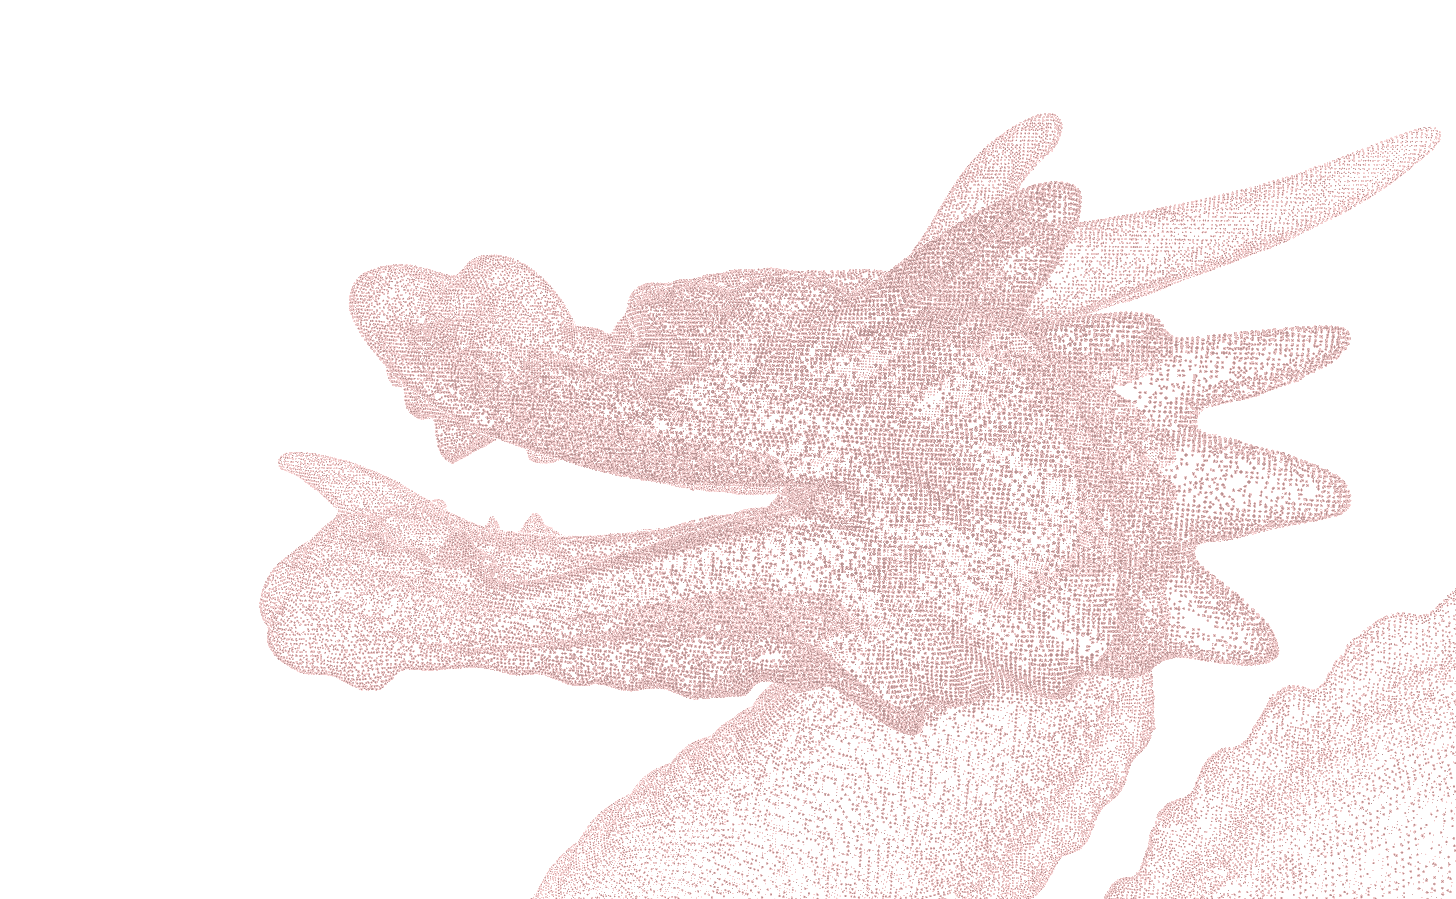
\includegraphics[width=.45\textwidth]{./Figures/point-cloud.png}}
	{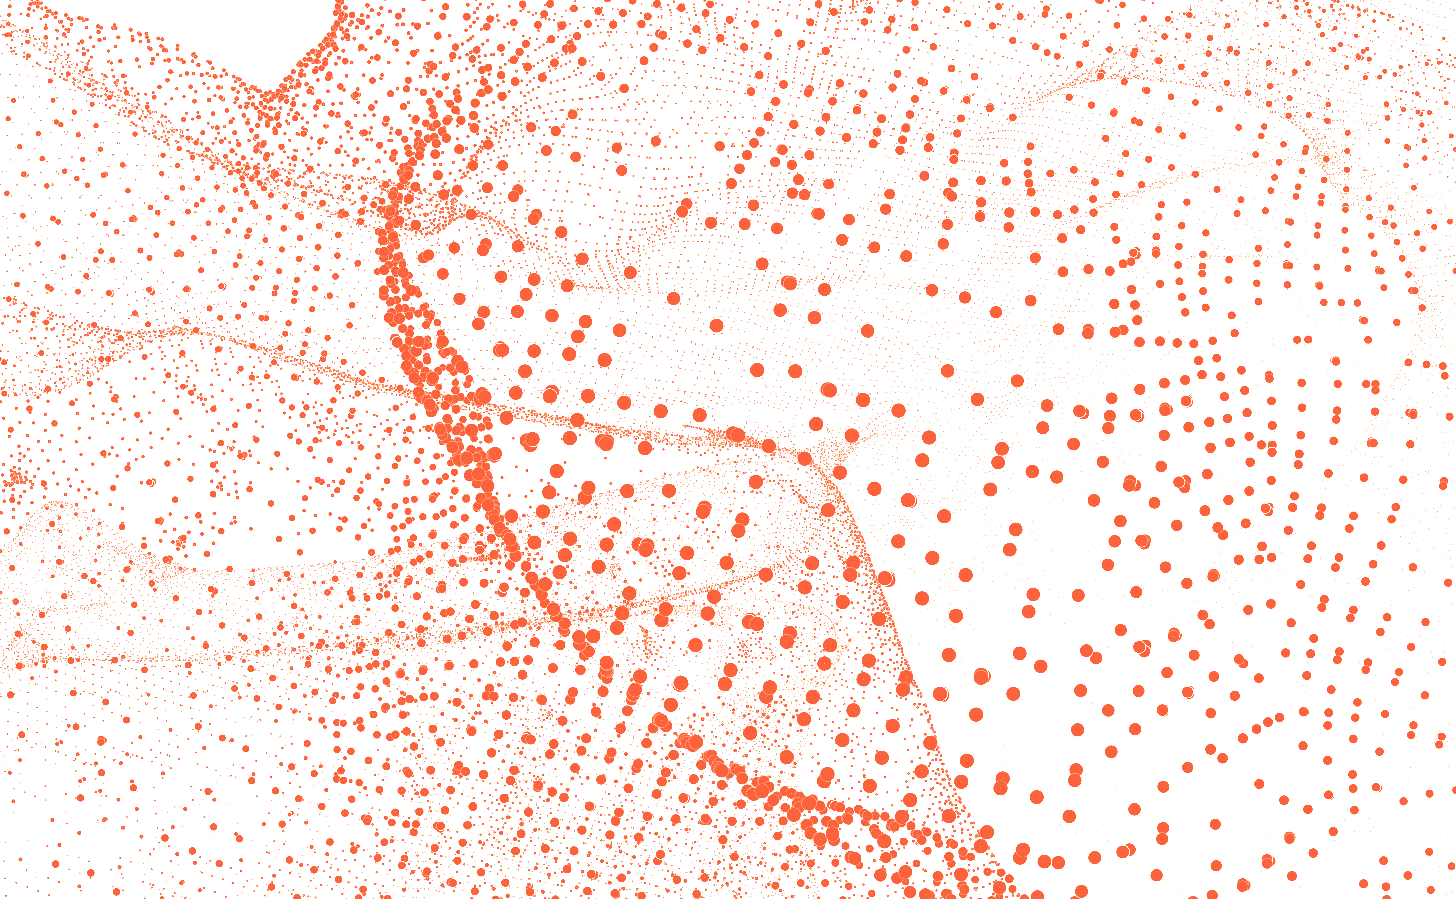
\includegraphics[width=.45\textwidth]{./Figures/point-cloud-zoom-in.png}}
	\decoRule
	\caption{Left: A piece of point cloud of the dragon object. Right: Zoom in of the point cloud.}
	\label{fig:point-cloud}
\end{figure}

%% introduce photometric stereo
Photometric stereo is another approach in computer vision which can be used for surface normal estimation, where the normals are inferred from appearance variations under multiple illuminations. The relative methods are typically solve the least square problem based on the pointwise image formation model.\cite{SFS} and based on the Bidirectional Reflectance Distribution Function (BRDF). While BRDF based model generally cannot account the global illumination effects and this is usually unavoidable problem due to the light interactions and difficult traced mathematically.

%% papers contribution, main work
Both directions mentioned above have been widely researched using deep learning approaches. However, the approach that takes both geometry and illuminated information together into account for normal estimation remains impoverishment. We present a deep learning based approach takes both geometry and photometric information into account for normal inference. For a practical reason, we consider only 1 illuminated image based on the calibrated camera and takes semi-dense point cloud as input data. To achieve this goal, we will mainly take the geometry information into consideration and take the photometric information as a supplementary.

%% introduce the network, trip-net, dataset
One of our challenge is to apply the semi-dense input data to the neural network in a image-wise way. UNet is a good network applying for computer vision task with up-sampling requirement. We modified it with gated activation unit called \textit{gated convolution layer (gconv)} to handle semi-dense input data. Another challenge is to merge the different input data feature maps together to cooperatively improved surface normal inference task. We propose a $ multi-fusion $ scheme for integration on separate feature map extractors. We will show that this multi-fusion design can be taken advantages of combination of different input data types and improved surface normal inference performance. To train our network, we create a synthetic RGB-D image dataset by utilizing one light source illumination and one ambient light illumination to simulate application scenarios. To simulate depth maps in real world, we applied uniform distributed drop-out noise to the input data with a control parameter for noise density.

%% experiments
We trained our approach on our proposed synthetic dataset ``synthetic-50-5" and evaluate it on 6 different metrics. We compare our approach against the geometry information based approach based on the similar network architecture and show that our calibrated illuminated RGB-D image based approach further improved normal accuracy. We also applied our model on real dataset and compare with the optimization based approach.

The structure of the thesis is as follows, Chapter 1 is the introduction of the whole work. Chapter 2 briefly discusses the related work about normal inference. Chapter 3 is the main approaches of this work. Chapter 4 introduces the created dataset for the training work. Chapter 5 is the description of the experiments and the evaluation of the models. Chapter 6 is the conclusion of the whole thesis.




% Chapter Template

\chapter{Related Work} % Main chapter title

\label{ch:02} % Change X to a consecutive number; for referencing this chapter elsewhere, use \ref{ChapterX}

%----------------------------------------------------------------------------------------
%	SECTION 1
%----------------------------------------------------------------------------------------

From PCA for estimation to recently deep learning based methods, the task of surface normal inference is also been well studied in last several decades. 


\section{Sparse Input processing}

%% methods deal with sparse input, like nconv, gconv ...
The depth map is supposed to be dense. Therefore, how to accept sparse depth map as input in CNNs is one of the most important problem. Some trivial solutions like median filters are good enough, if the missing pixels are sparse enough, however, for the case of huge missing holes in the depth map, it produces just a paltry result. Thus a reasonable guess is required for missing areas. Generally, it can be solved as image inpainting problems,\cite{inpainting1},\cite{inpainting2}. 

%% Deep learning based approaches
Some deep learning based method for image inpainting also achieved quite good performance for the hole mending task. 
%% talk about gconv
Notably, in 2016, Oord et al. \cite{gated_activation} proposed a gated activation unit for a CNN model,
\[\textbf{y} = \tanh (W_{k,f} * \textbf{x}) \odot \sigma (W_{k,g} * \textbf{x})\]
to substitute the standard activation layer, where $ \sigma $ is the sigmoid function, which constricts the output value of second part between $ [0,1] $.  The function is inspired by Long Short-Term Memory (LSTM) \cite{lstm} and Rated Recurrent Unit (GRU).\cite{gru} It is originally used for learning complex interactions as LSTM gates does. In 2018, Yu et al. \cite{gconv} employed same function for free-form image inpainting, which can be used to learn mask automatically from image it self.

%% talk about nconv
Different to aforementioned approaches, Knutsson et al. in 2005 introduced normalized convolution \cite{nconv} dealing with missing sample case for convolution operation, which aims to reconstruct the missing pixels from the sparse output sensed by cameras, which particularly considered the confidence of each interpolated pixels, since it provides the trustworthiness of the predicted value. The higher the reliability of the value inference, the better the model shape reconstruction.

In 2018, Eldesokey et al. \cite{ncnn} applied normalized convolution in CNN as normalized convolution layer that takes both sparse depth map and a binary confidence map as input to perform scene depth completion.
In 2020, Eldesokey et al. \cite{pncnn} focus on modeling the uncertainty of depth data instead of assuming binary input confidence.

Guided method \cite{guided} requires addition information like RGB image or the certainty map of depth map, and fuse them together to predict the dense depth map.




\section{Normal Inference}

%% normal estimation method introduction
Usually, we based on point cloud, depth map or RGB/Grayscale image of the objects or scenes to inference the normals. 

Traditional methods evaluate normals based on neighbor information of point cloud or depth map.
In 2012, Holzer et al. \cite{Holzer.S} proposed method to calculate normal from covariance matrices. 
This method use integral image as input, which is able to run algorithm in a high frame speed. They smooth the depth data in order to handle the noise of depth image. The drawbacks are, as mentioned in the paper, the normals error go up when point depths change severely. In 2013, Fouhey et al. \cite{geometry_based_solution} proposed a method constructing a over-determined function systems to predict normals and solving it 
by algebra methods. Similarly, this approach gives a quick but coarse normal inference. 


%% CNN based methods
Recently, CNN based methods improve the performance of image processing to a brand new stage. In 2014, Eigen et al.\cite{Eigen} proposed a method predicting depth map directly from RGB image using CNN. In this case, no depth map is required. In 2016, Laina et al. \cite{img2depth} proposed a deeper network based on ResNet \cite{resnet} with a well designed upsamling part. 
%% guided scene completion
In 2018, Qi et al. proposed GeoNet\cite{GeoNet}, it integrates both algebra method and also CNN method to inference depthmap based on \cite{img2depth} \cite{geometry_based_solution}. 

%% upsampling 
It is worth to noticed that, the output of normal inference CNN model is not one or severl labels but an entire image or normal map with same size. 
%% talk about image upsampling, unet
Recently, Ronneberger et al proposed an architecture called UNet \cite{unet} for biomedical image segmentations. The architecture is shown in Figure \ref{fig:u-net}.The first half network is a usual classification convolutional network, the second half replace the pooling layers and traditional fc layers in the traditional CNNs to upsampling layers, thus in the end of the second half, the output is able to back to the input size. The proposed network can successfully assigned each pixel a class for segmentation tasks. Under this symmetric network, an input image is downsampled 3 times and upsampled 3 times. Output image has exactly the same size as input image. The downsampling and upsampling both have large number of feature channels, which guarantee the network propagates the information to higher resolution layers.


%%\begin{figure}[!h]
%%	\centering
%%	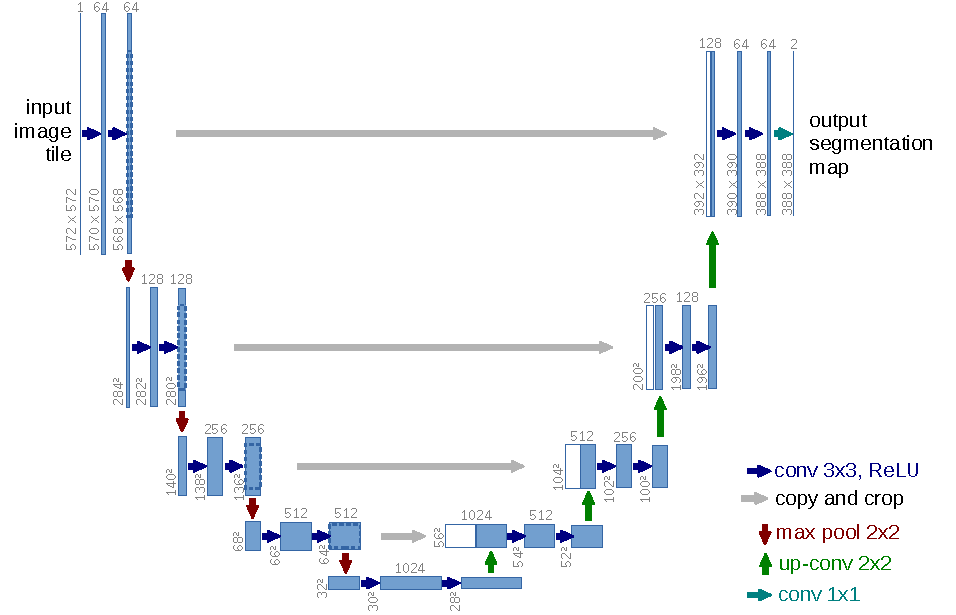
\includegraphics[width=\textwidth]{./ref/u-net-illustration-correct-scale2}
%%	\caption{U-net architecture (example for 32x32 pixels in the lowest resolution). Each blue box corresponds to a multi-channel feature map. The number of channels is denoted on top of the box. The x-y-size is provided at the lower left edge of the box. White boxes represent copied feature maps. The arrows denote the different operations.
	%%	}
%%	\label{fig:u-net}
%% \end{figure}



%% unstructured point cloud 
In some case, the input is unstructured point cloud which can not be fed into a CNN entirely. Thus, a challenge task connect to the deep learning is the input format. Since different point clouds have different sizes. 
In 2018, Ben-Shabat et al. \cite{Ben-Shabat_2019_CVPR} presented Nesti-Net. It predicts the normal point by point with the help of neighbor points. It fixed the distance of considering neighbors to provide an unified input for CNN. In 2021, Zhou et al. \cite{zhou2021fast} presents a method considering overlapping of different patches (a group of neighboring points) as input to evaluate normals. 
 
% Chapter Template

\chapter{Approaches} % Main chapter title

\label{ch:03} % Change X to a consecutive number; for referencing this chapter elsewhere, use \ref{ChapterX}


The normal inference task can be simply stated as follows:

Given a structured point cloud $ V^{W\times H\times 3} $,
We would like to estimate the normal map  $ N^{W\times H \times 3} $, where each normal  $ \textbf{n}^{3\times 1} $ at point $ \textbf{p}^{3\times 1} $ is a unit vector with direction point outward and perpendicular to the tangent plane of the surface at point $ \textbf{p}^{3\times 1} $.

In this chapter, we first introduced an optimization based method using singular value decomposition (SVD). Then, we introduced the main work of this thesis, a deep learning based method which use gated convolution layers for normal inference. 

\section{Neighbor based surface normal estimation}

For a point $ \textbf{p} $ in a surface, its normal $ \textbf{n} $ is a vector of the tangent plane $ \Pi $ of the surface at this point $ \textbf{p} $. As long as find $ k $ vectors $ \textbf{v}_1, ..., \textbf{v}_k \in \mathbb{R}^3 $ on the same tangent plane, the normal can be calculated immediately by solving equation system $ A \cdot \textbf{n} = 0 $, where $ A \in \mathbb{R}^{k\times 3} $ is the vector matrix vertically stacked by $ \textbf{v}_1, ..., \textbf{v}_k $.

In order to find the vectors on the tangent plane, we can assume the $ k $ neighbor points of $ \textbf{p} $ are in the same plane, where $ k $ is a customized parameter. Then, 
\begin{equation}
	\textbf{v}_i = \textbf{p}_i - \textbf{p} \quad \text{for} \ 1 \le i \le k
\end{equation}
are $ k $ vectors on the tangent plane. Since they all perpendicular to the normal $ \textbf{n} $, we have 
\begin{equation}{\label{eq:normal-overdetermined-equation}}
	\textbf{v}_i \cdot \textbf{n} = 0 \quad \text{for} \ 1 \le i \le k
\end{equation}
The equation system can be further simplified as 
\begin{equation}{\label{eq:normal-overdetermined-equation}}
	A \cdot \textbf{n} = 0
\end{equation}
where $ A\in \mathbb{R}^{k\times 3} $ denotes the matrix constructed by $ \textbf{v}_i $.
In order to avoid trivial solution, one more constraint should be added
\[ \|  \bn_{3 \times 1} \|_2^2 = 1  \]
which also let the normal to be a unit vector.

To calculate a valid normal, at least 3 points are required, i.e. $ k>=3 $. For the sake of robust, more points can be used to reduce the measuring error. For the case $ k>3 $, the equation system is usually over-determined, then the equation system mentioned above can be converted to follow optimization problem
\begin{equation}
	\begin{array}{rrclcl}
		\displaystyle \min & \multicolumn{3}{l}{\| A  \bn \|^2} \\
		\\
		\textrm{s.t.} & \| \bn \|^2 & = & 1 
	\end{array}
\end{equation}
which can be solved by singular value decomposition(SVD). Let the decomposition of $ A=U\Sigma V^T $, The solution i.e. normal is the last column of $ V $.


At last, all the normals should point ot view point $ \textbf{s} $, thus the direction of a normal should be inverted if 
\begin{equation}\label{eq:normal-invertion}
	\textbf{n} \cdot (\textbf{p}  - \textbf{s}) > 0
\end{equation}

Repeat the procedure for all the points in the point cloud to get the entire normal map. 

% ---------------------------- gated convolution neural network -------------------------------------------------
\section{Gated Convolution neural network for surface normal estimation}
\label{gcnn}


\cite{gated_activation} proposed a gated activation unit to model more complex interactions comparing to standard CNN layers, which mainly inspired by the multiplicative units exist in Long Short-Term Memory proposed by \cite{lstm} and Rated Recurrent Unit (GRU) proposed by \cite{gru}. 
\cite{gconv} employed the same gated unit solving for the free-form image inpainting task. The proposed network use 3 channel RGB images as input and estimate the missing pixels. 


Recently, deep learning based method achieved a great succeed for image processing.  \cite{yolov3} proposed  \cite{efficientDet} These network architectures use a batch of RGB/Grayscale images as input and are employed for classification problems. Usually, the images are convoluted with a convolution layer and downsampling with pooling layers. The outputs of the network consist of a single value to represent the index of the corresponding class \cite{efficientDet}, or with a set of values to represent the position of bounding boxes.\cite{yolov3}. However, in many other vision tasks, like normal map inference, the output is demanded as the same shape as the input. Instead of predicting one or several classes for the whole input matrix, the class for each pixel requires for prediction. In this case, the traditional network architecture is not suitable anymore.





%% upsampling 
It is worth to noticed that, the output of normal inference CNN model is not one or severl labels but an entire image or normal map with same size. 
%% talk about image upsampling, unet
Recently, Ronneberger et al proposed an architecture called UNet \cite{unet} for biomedical image segmentations. The architecture is shown in Figure \ref{fig:u-net}.The first half network is a usual classification convolutional network, the second half replace the pooling layers and traditional fc layers in the traditional CNNs to upsampling layers, thus in the end of the second half, the output is able to back to the input size. The proposed network can successfully assigned each pixel a class for segmentation tasks. Under this symmetric network, an input image is downsampled 3 times and upsampled 3 times. Output image has exactly the same size as input image. The downsampling and upsampling both have large number of feature channels, which guarantee the network propagates the information to higher resolution layers.



The standard convolution layer goes like this

\begin{equation}
	\begin{array}{rrclcl}
		\displaystyle O = \Sigma\Sigma W\cdot I \\
	\end{array}
\end{equation}
each filter is applied as a sliding window to walk through the whole matrix and calculates the output matrix. Every entry in the matrix counts in the operation. This is reasonable for image processing task with full-dense input, since no missing pixels exist. 
However, the depth-map and point cloud is only semi-dense. The valid and invalid pixels will be treated equally if we still perform standard convolution layers. Since the aim of the network is not learning the pattern of noise, but the noise with eternally changing patterns will confuse the network, and it fails the normal inference, a mask is required to distinguish two kinds of pixels. 


% why we need a mask
\cite{pncnn0} use binary mask to indicate valid pixels, and further use normalized convolution to predict the output. The normalized convolution is shown as follows

\begin{equation}
	\begin{array}{rrclcl}
		O(x,y) = 
		\begin{cases}
			\dfrac{\Sigma_i^k\Sigma_j^k W(i,j) \cdot I(x-i,y-j) \cdot M(x-i,y-j)}{\Sigma_i^k\Sigma_j^k W(i,j) \cdot M(x-i,y-j)}, & \text{if}\ \sum_{i}^k\sum_{j}^k M(i,j)>0 \\
			0, & \text{otherwise}
		\end{cases}
	\end{array}
\end{equation}

where $ k $ is the kernel size, $ (x,y) $ is the position in input, $ (i,j) $ is the displacement in kenel, $ M $ is the corresponding mask. A binary mask uses 1 to indicate valid pixels and 0 otherwise. $ \odot $ denotes element-wise multiplication.

Normalized convolution layer added the weight to the mask. However, a initialization for the mask is still required, and the propagation of the mask remain a tricky task. 
\subsection{Gated Convolution}

% introduce gconv
\cite{gconv} proposed gated convolution using for image inpainting task. 

The structure is shown in Figure \ref{fig:gconvLayer}. Instead of using a mask as input to indicate valid pixels, it employs a standard convolution layers to learn this mask directly from data. The valid pixels are then activated by a Sigmoid function. Then it imply element-wise multiplication with the feature map. Formally, the gated convolution is described as follows, the layer with input size $ (N, C_{in}, H, W) $ and output size $ (N, C_{out}, H_{out}, W_{out}) $:
\begin{equation}\label{gconv}
	o(N_i, C_{o_j}) = \sigma(\sum_{k=0}^{C_{in}-1}w_g(C_{o_j}, k) \star i(N_i,k) + b_g(C_{o_j})) * 
	\phi (\sum_{k=0}^{C_{in}-1}w_f(C_{o_j}, k) \star i(N_i,k) + b_f(C_{o_j}))
\end{equation}
where $ \phi $ is LeakyReLU function, $ \sigma $ is sigmoid function, thus the output values are in range $ [0,1] $, $ \star $ is the valid 2D cross-correlation operator, $ N $ is batch size, $ C $ denotes a number of channels, $ H $ is a height of input planes in pixels, and $ W $ is width in pixels, $ w(C_{o_j},k) $ denotes the weight of $ j $-th output channel corresponding $ k $-th input channel, $ i(N_i, k) $denotes the input of $ i $-th batch corresponding $ k $-th input channel, $ b(C_{o_j}) $ denotes the bias of $ j $-th output channel.


% Gated Convolution Layer
\begin{figure}[h!]
	\centering
	\begin{tikzpicture}
		\tikzstyle{rect} = [rectangle, rounded corners, minimum width=3cm, minimum height=1cm,text centered, draw=black, fill=blue!20]
		\tikzstyle{arrow} = [thick,->,>=stealth]
		\node (output) [rect] {Output};
		\node (oplus) [below of=output, yshift=-.5cm] {$\Huge\oplus $};
		\node (LeakyReLU) [rect,below of=oplus, yshift=-1cm] {Feature};
		\node (sigmoid) [rect, below of=oplus, yshift=-1cm, xshift=-4cm] {Mask};
		
		\node (conv1) [rect,below of=sigmoid, yshift=-1cm] {Mask};
		\node (conv2) [rect,below of=LeakyReLU, yshift=-1cm] {Feature};
		\node (input) [below of=oplus] at (0,-8) {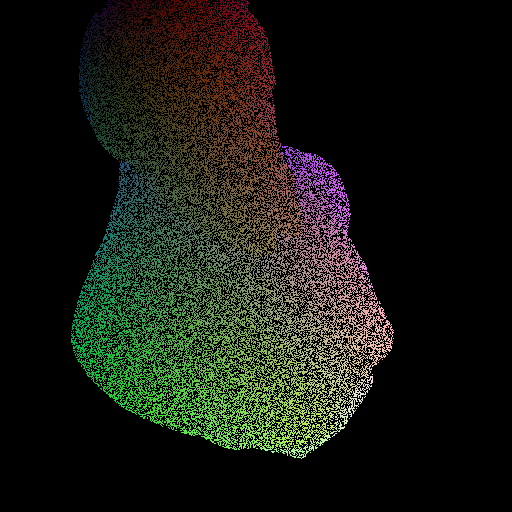
\includegraphics[width=.25\textwidth]{./Figures/train-input.png}};
		
		\draw [arrow] (oplus) -- (output);
		\draw [arrow] (sigmoid) |- (oplus);
		\draw [arrow] (LeakyReLU) -- (oplus);
		\draw [arrow] (conv2) --  node [text width=2.5cm, midway, right=1em]{LeakyReLU} (LeakyReLU);
		\draw [arrow] (conv1) --  node [text width=2.5cm, midway, right=1em]{Sigmoid} (sigmoid);
		\draw [arrow] (input) -|  node [text width=2.5cm, midway, below=1em]{Conv2D} (conv1);
		\draw [arrow] (input) -- node [text width=2.5cm, midway, right=1em]{Conv2D} (conv2);
	\end{tikzpicture}
	\caption{Gated Convolution Layer, where $ \oplus $ denotes element-wise multiplication.}
	\label{fig:gconvLayer}
\end{figure}

%\section{Canny Edge Detection for Detail Enhancement}
%The inaccuracy part is usually concentrate in the coarse surface or drastic changed surface parts of the object. The corresponding part can be extracted separately via edge detector algorithms, like Canny Edge detector. Feed the edges to a special net for normal prediction might improve the accuracy further. 

\subsection{Architecture}
\label{sec:architecture}
Based on the implementation mentioned above, the architecture roughly follows on UNet proposed by \cite{unet}, as shown in Figure \ref{fig:gcnn-archi}. 

Instead of using pooling layers for down/up samplings, gated convolution layer with stride $ (2,2) $ is used. The gated convolution using Sigmoid function for gating layer and LeakyReLU function for feature layer. All the layers are gated convolution layer with the exception of last two layer, which instead uses standard convolution layer to scale the output in range $\left[-1, 1\right]$. Other than the last two layers which use $ 1\times 1 $ kernels, all the gated convolution layer use $ 3\times 3 $ kernels with $ 1\times1 $ padding. 

The input is 3D vertex with size $ 512\times512\times3 $, and output is $ 512\times512\times3 $ normal map, which has the same resolution. There are 3 times downsamplings, each scale with 3 gated convolution layers, the third layer has stride-2. The upsampling part interpolate the feature maps 3 times with 1 gated convolution layer in each scale. 

It keeps the skip connection in UNet to remain the fine detail features. 
 
% GCNN Architecture
\begin{figure}[!h]
	\centering
	%% https://tex.stackexchange.com/questions/12020/what-is-the-easiest-way-to-draw-a-3d-cube-with-tikz
	\begin{tikzpicture}
		%% -------------------------------------- parameters ------------------------------------------------
		\pgfmathsetmacro{\vdist}{0.4}
		
		\pgfmathsetmacro{\boxsizea}{3}	%% width 512
		\pgfmathsetmacro{\boxsizeb}{1.5}	%% width 256
		\pgfmathsetmacro{\boxsizec}{1}	%% width 128
		\pgfmathsetmacro{\boxsized}{0.7}	%% width 64
		
		
		\pgfmathsetmacro{\boxwidthd}{0.1}	%% width 1
		\pgfmathsetmacro{\boxwidtha}{0.2}	%% width 3
		\pgfmathsetmacro{\boxwidthb}{\boxwidtha*1.3}	%% width 32
		\pgfmathsetmacro{\boxwidthc}{\boxwidtha*3}		%% width 64
		
		\pgfmathsetmacro{\convwshift}{9}
		\pgfmathsetmacro{\preprocessingshift}{4}
		\pgfmathsetmacro{\labelshift}{1.5}
		\pgfmathsetmacro{\gconvwshift}{0}
		
		\pgfmathsetmacro{\secrowshift}{-6}
		
		\pgfmathsetmacro{\convrowstart}{4}
		\pgfmathsetmacro{\secondrowstart}{4}
		
		%% https://www.tug.org/pracjourn/2007-4/walden/color.pdf
		\definecolor{gconvcolor}{rgb}{0.5,0.7,0.7}
		\definecolor{convcolor}{rgb}{0.5,0.7,0.3}
		\definecolor{gconvdilatedcolor}{rgb}{0.6,0,0.3}
		
		
		%% ---------------------------------- preprocessing --------------------------------------------
		%%  img_in 1x512x512
		\pgfmathsetmacro{\disttimes}{3.5}
		\pgfmathsetmacro{\yschift}{\preprocessingshift}
		\node[inner sep=0pt] (depthmap) at (\vdist*\disttimes,\yschift)
		{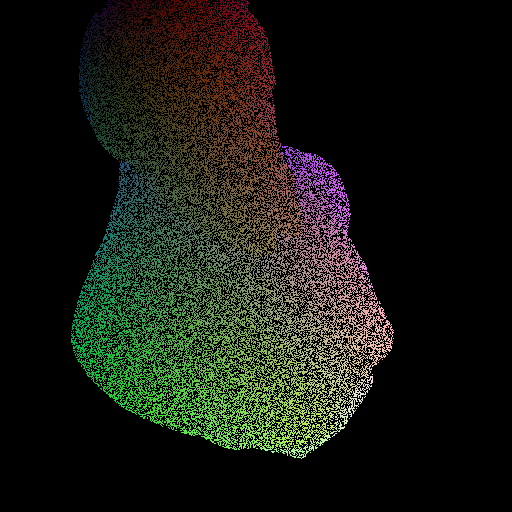
\includegraphics[width=.15\textwidth]{./Figures/train-input.png}};
		\node[text width=3.5cm] at (\vdist*\disttimes+1,\yschift-1.5) {3D Vertex};
		
		\draw [-stealth](1.45,\yschift-1.8) -- (1.45,\yschift-2.6);
		
		\draw [-stealth]  (\vdist*\disttimes+1.6,\yschift) -- (\vdist*\disttimes+1.1,\yschift);
		
		\pgfmathsetmacro{\disttimes}{10}
		\pgfmathsetmacro{\yschift}{\preprocessingshift}
		\node[inner sep=0pt] (depthmap) at (\vdist*\disttimes,\yschift)
		{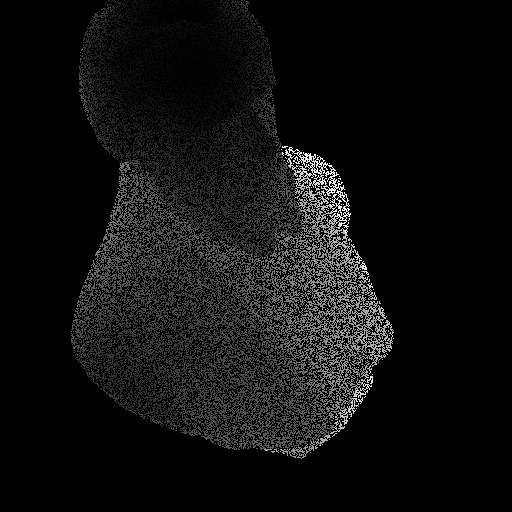
\includegraphics[width=.15\textwidth]{./Figures/train-depth-noise}};
		\node[text width=3.5cm] at (\vdist*\disttimes+1,\yschift-1.5) {Add Noise};
		
		\draw [-stealth] (\vdist*\disttimes+1.6,\yschift) -- (\vdist*\disttimes+1.1,\yschift);
		
		\pgfmathsetmacro{\disttimes}{16.5}
		\pgfmathsetmacro{\yschift}{\preprocessingshift}
		\node[inner sep=0pt] (depthmap) at (\vdist*\disttimes,\yschift)
		{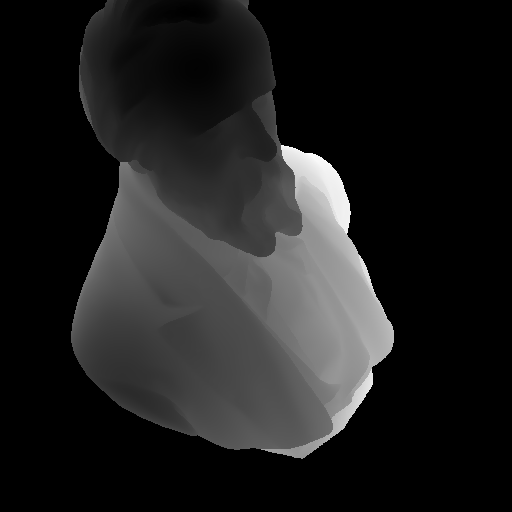
\includegraphics[width=.15\textwidth]{./Figures/train-depth.png}};
		\node[text width=2cm] at (\vdist*\disttimes+0.2,\yschift-1.5) {Depth Map};
		
		
		%% ----------------------------------- output normal map -------------------------------------
		\pgfmathsetmacro{\disttimes}{25}
		\pgfmathsetmacro{\yschift}{\preprocessingshift}
		\node[inner sep=0pt] (depthmap) at (\vdist*\disttimes,\yschift)
		{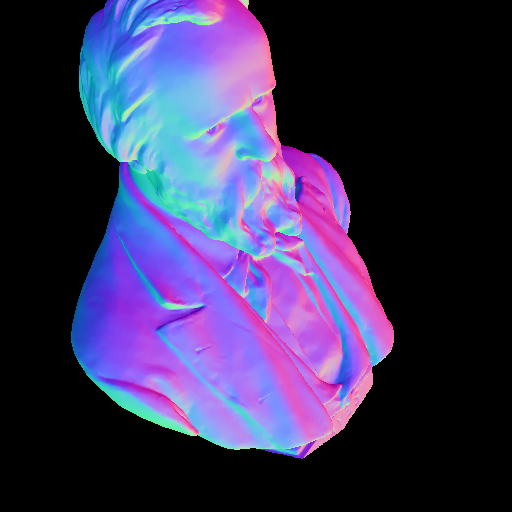
\includegraphics[width=.15\textwidth]{./Figures/train-normal-gt.png}};
		\node[text width=2.5cm] at (\vdist*\disttimes,\yschift-1.5) {Normal Map};
		
		\draw [-stealth] (\vdist*\disttimes+0.2,\yschift-2.7) -- (\vdist*\disttimes+0.2,\yschift-1.8);
		
		
		%% ------------------------------------------- vertex input ----------------------------------------------
		%% 	d_in							3x512x512
		%%	dconv1: 	d_in-->x1 			32x512x512
		\pgfmathsetmacro{\disttimes}{1}	%% width 32
		\pgfmathsetmacro{\boxsize}{\boxsizea}	%% size 512
		\pgfmathsetmacro{\boxwidth}{\boxwidthb}	%% width 32
		\pgfmathsetmacro{\yschift}{\gconvwshift}
		\node[text width=1cm] at (\vdist*\disttimes+0.1,\yschift-3.5) {32};
		\draw[black, fill=gconvcolor] (\vdist*\disttimes,\yschift,0) -- ++(-\boxwidth,0,0) -- ++(0,-\boxsize,0) -- ++(\boxwidth,0,0) -- cycle;
		\draw[black, fill=gconvcolor] (\vdist*\disttimes,\yschift,0) -- ++(0,0,-\boxsize) -- ++(0,-\boxsize,0) -- ++(0,0,\boxsize) -- cycle;
		\draw[black, fill=gconvcolor] (\vdist*\disttimes,\yschift,0) -- ++(-\boxwidth,0,0) -- ++(0,0,-\boxsize) -- ++(\boxwidth,0,0) -- cycle;
		
		%%	dconv2:		x1-->x1				32x512x512
		\pgfmathsetmacro{\disttimes}{2}	%% width 32
		\pgfmathsetmacro{\boxsize}{\boxsizea}	%% size 512
		\pgfmathsetmacro{\boxwidth}{\boxwidthb}	%% width 32
		\pgfmathsetmacro{\yschift}{\gconvwshift}
		\draw[black, fill=gconvcolor] (\vdist*\disttimes,\yschift,0) -- ++(-\boxwidth,0,0) -- ++(0,-\boxsize,0) -- ++(\boxwidth,0,0) -- cycle;
		\draw[black, fill=gconvcolor] (\vdist*\disttimes,\yschift,0) -- ++(0,0,-\boxsize) -- ++(0,-\boxsize,0) -- ++(0,0,\boxsize) -- cycle;
		\draw[black, fill=gconvcolor] (\vdist*\disttimes,\yschift,0) -- ++(-\boxwidth,0,0) -- ++(0,0,-\boxsize) -- ++(\boxwidth,0,0) -- cycle;
		
		%%	dconv3:		x1-->x1				32x512x512
		\pgfmathsetmacro{\disttimes}{3}	%% width 32
		\pgfmathsetmacro{\boxsize}{\boxsizea}	%% size 512
		\pgfmathsetmacro{\boxwidth}{\boxwidthb}	%% width 32
		\pgfmathsetmacro{\yschift}{\gconvwshift}
		\draw[black, fill=gconvcolor] (\vdist*\disttimes,\yschift,0) -- ++(-\boxwidth,0,0) -- ++(0,-\boxsize,0) -- ++(\boxwidth,0,0) -- cycle;
		\draw[black, fill=gconvcolor] (\vdist*\disttimes,\yschift,0) -- ++(0,0,-\boxsize) -- ++(0,-\boxsize,0) -- ++(0,0,\boxsize) -- cycle;
		\draw[black, fill=gconvcolor] (\vdist*\disttimes,\yschift,0) -- ++(-\boxwidth,0,0) -- ++(0,0,-\boxsize) -- ++(\boxwidth,0,0) -- cycle;
		
		\draw (\vdist*\disttimes-0.2,\yschift-3.2) -- (\vdist*\disttimes-0.2,\yschift-4);
		\draw (\vdist*\disttimes-0.2,\yschift-4) -- (\vdist*\disttimes+6.5,\yschift-4);
		\draw [-stealth] (\vdist*\disttimes+6.5,\yschift-4) -- (\vdist*\disttimes+6.5,\yschift-3.2);
		
		
		%% downsample 1
		%%	dconv4:		x1-->x2				32x256x256
		\pgfmathsetmacro{\disttimes}{4}	%% width 32
		\pgfmathsetmacro{\boxsize}{\boxsizeb}	%% size 256
		\pgfmathsetmacro{\boxwidth}{\boxwidthb}	%% width 32
		\pgfmathsetmacro{\yschift}{\gconvwshift-0.5}	%% width 32
		\draw[black, fill=gconvcolor] (\vdist*\disttimes,\yschift,0) -- ++(-\boxwidth,0,0) -- ++(0,-\boxsize,0) -- ++(\boxwidth,0,0) -- cycle;
		\draw[black, fill=gconvcolor] (\vdist*\disttimes,\yschift,0) -- ++(0,0,-\boxsize) -- ++(0,-\boxsize,0) -- ++(0,0,\boxsize) -- cycle;
		\draw[black, fill=gconvcolor] (\vdist*\disttimes,\yschift,0) -- ++(-\boxwidth,0,0) -- ++(0,0,-\boxsize) -- ++(\boxwidth,0,0) -- cycle;
		%%	dconv2:		x2-->x2				32x256x256
		\pgfmathsetmacro{\disttimes}{5}	%% width 32
		\pgfmathsetmacro{\boxsize}{\boxsizeb}	%% size 256
		\pgfmathsetmacro{\boxwidth}{\boxwidthb}	%% width 32
		\pgfmathsetmacro{\yschift}{\gconvwshift-0.5}	%% width 32
		\draw[black, fill=gconvcolor] (\vdist*\disttimes,\yschift,0) -- ++(-\boxwidth,0,0) -- ++(0,-\boxsize,0) -- ++(\boxwidth,0,0) -- cycle;
		\draw[black, fill=gconvcolor] (\vdist*\disttimes,\yschift,0) -- ++(0,0,-\boxsize) -- ++(0,-\boxsize,0) -- ++(0,0,\boxsize) -- cycle;
		\draw[black, fill=gconvcolor] (\vdist*\disttimes,\yschift,0) -- ++(-\boxwidth,0,0) -- ++(0,0,-\boxsize) -- ++(\boxwidth,0,0) -- cycle;
		%%	dconv3:		x2-->x2				32x256x256
		\pgfmathsetmacro{\disttimes}{6}	%% width 32
		\pgfmathsetmacro{\boxsize}{\boxsizeb}	%% size 256
		\pgfmathsetmacro{\boxwidth}{\boxwidthb}	%% width 32
		\pgfmathsetmacro{\yschift}{\gconvwshift-0.5}	%% width 32
		\draw[black, fill=gconvcolor] (\vdist*\disttimes,\yschift,0) -- ++(-\boxwidth,0,0) -- ++(0,-\boxsize,0) -- ++(\boxwidth,0,0) -- cycle;
		\draw[black, fill=gconvcolor] (\vdist*\disttimes,\yschift,0) -- ++(0,0,-\boxsize) -- ++(0,-\boxsize,0) -- ++(0,0,\boxsize) -- cycle;
		\draw[black, fill=gconvcolor] (\vdist*\disttimes,\yschift,0) -- ++(-\boxwidth,0,0) -- ++(0,0,-\boxsize) -- ++(\boxwidth,0,0) -- cycle;
		
		\draw (\vdist*\disttimes-0.1,\yschift-1.6) -- (\vdist*\disttimes-0.1,\yschift-2.7);
		\draw (\vdist*\disttimes-0.1,\yschift-2.7) -- (\vdist*\disttimes+4.2,\yschift-2.7);
		\draw [-stealth] (\vdist*\disttimes+4.2,\yschift-2.7) -- (\vdist*\disttimes+4.2,\yschift-1.7);
		
		
		%% downsample 2
		%%	dconv4:		x2-->x3				32x128x128
		\pgfmathsetmacro{\disttimes}{7}	%% width 32
		\pgfmathsetmacro{\boxsize}{\boxsizec}	%% size 128
		\pgfmathsetmacro{\boxwidth}{\boxwidthb}	%% width 32
		\pgfmathsetmacro{\yschift}{\gconvwshift-0.8}	%% width 32
		\draw[black, fill=gconvcolor] (\vdist*\disttimes,\yschift,0) -- ++(-\boxwidth,0,0) -- ++(0,-\boxsize,0) -- ++(\boxwidth,0,0) -- cycle;
		\draw[black, fill=gconvcolor] (\vdist*\disttimes,\yschift,0) -- ++(0,0,-\boxsize) -- ++(0,-\boxsize,0) -- ++(0,0,\boxsize) -- cycle;
		\draw[black, fill=gconvcolor] (\vdist*\disttimes,\yschift,0) -- ++(-\boxwidth,0,0) -- ++(0,0,-\boxsize) -- ++(\boxwidth,0,0) -- cycle;
		%%	dconv2:		x3-->x3				32x128x128
		\pgfmathsetmacro{\disttimes}{8}	%% width 32
		\pgfmathsetmacro{\boxsize}{\boxsizec}	%% size 128
		\pgfmathsetmacro{\boxwidth}{\boxwidthb}	%% width 32
		\pgfmathsetmacro{\yschift}{\gconvwshift-0.8}	%% width 32
		\draw[black, fill=gconvcolor] (\vdist*\disttimes,\yschift,0) -- ++(-\boxwidth,0,0) -- ++(0,-\boxsize,0) -- ++(\boxwidth,0,0) -- cycle;
		\draw[black, fill=gconvcolor] (\vdist*\disttimes,\yschift,0) -- ++(0,0,-\boxsize) -- ++(0,-\boxsize,0) -- ++(0,0,\boxsize) -- cycle;
		\draw[black, fill=gconvcolor] (\vdist*\disttimes,\yschift,0) -- ++(-\boxwidth,0,0) -- ++(0,0,-\boxsize) -- ++(\boxwidth,0,0) -- cycle;
		%%	dconv3:		x3-->x3				32x128x128
		\pgfmathsetmacro{\disttimes}{9}	%% width 32
		\pgfmathsetmacro{\boxsize}{\boxsizec}	%% size 128
		\pgfmathsetmacro{\boxwidth}{\boxwidthb}	%% width 32
		\pgfmathsetmacro{\yschift}{\gconvwshift-0.8}	%% width 32
		\draw[black, fill=gconvcolor] (\vdist*\disttimes,\yschift,0) -- ++(-\boxwidth,0,0) -- ++(0,-\boxsize,0) -- ++(\boxwidth,0,0) -- cycle;
		\draw[black, fill=gconvcolor] (\vdist*\disttimes,\yschift,0) -- ++(0,0,-\boxsize) -- ++(0,-\boxsize,0) -- ++(0,0,\boxsize) -- cycle;
		\draw[black, fill=gconvcolor] (\vdist*\disttimes,\yschift,0) -- ++(-\boxwidth,0,0) -- ++(0,0,-\boxsize) -- ++(\boxwidth,0,0) -- cycle;
		
		\draw (\vdist*\disttimes-0.1,\yschift-1.2) -- (\vdist*\disttimes-0.1,\yschift-1.8);
		\draw (\vdist*\disttimes-0.1,\yschift-1.8) -- (\vdist*\disttimes+1.8,\yschift-1.8);
		\draw [-stealth] (\vdist*\disttimes+1.8,\yschift-1.8) -- (\vdist*\disttimes+1.8,\yschift-1.2);
		
		
		%% downsample 3
		%%	dconv4:		x3-->x4				32x64x64
		\pgfmathsetmacro{\disttimes}{10}
		\pgfmathsetmacro{\boxsize}{\boxsized}	%% size 64
		\pgfmathsetmacro{\boxwidth}{\boxwidthb}	%% width 32
		\pgfmathsetmacro{\yschift}{\gconvwshift-1}
		\draw[black, fill=gconvcolor] (\vdist*\disttimes,\yschift,0) -- ++(-\boxwidth,0,0) -- ++(0,-\boxsize,0) -- ++(\boxwidth,0,0) -- cycle;
		\draw[black, fill=gconvcolor] (\vdist*\disttimes,\yschift,0) -- ++(0,0,-\boxsize) -- ++(0,-\boxsize,0) -- ++(0,0,\boxsize) -- cycle;
		\draw[black, fill=gconvcolor] (\vdist*\disttimes,\yschift,0) -- ++(-\boxwidth,0,0) -- ++(0,0,-\boxsize) -- ++(\boxwidth,0,0) -- cycle;
		%%	dconv2:		x4-->x4				32x64x64
		\pgfmathsetmacro{\disttimes}{11}
		\pgfmathsetmacro{\boxsize}{\boxsized}	%% size 64
		\pgfmathsetmacro{\boxwidth}{\boxwidthb}	%% width 32
		\pgfmathsetmacro{\yschift}{\gconvwshift-1}	%% width 32
		\draw[black, fill=gconvcolor] (\vdist*\disttimes,\yschift,0) -- ++(-\boxwidth,0,0) -- ++(0,-\boxsize,0) -- ++(\boxwidth,0,0) -- cycle;
		\draw[black, fill=gconvcolor] (\vdist*\disttimes,\yschift,0) -- ++(0,0,-\boxsize) -- ++(0,-\boxsize,0) -- ++(0,0,\boxsize) -- cycle;
		\draw[black, fill=gconvcolor] (\vdist*\disttimes,\yschift,0) -- ++(-\boxwidth,0,0) -- ++(0,0,-\boxsize) -- ++(\boxwidth,0,0) -- cycle;
		%%	dconv3:		x4-->x4				32x64x64
		\pgfmathsetmacro{\disttimes}{12}
		\pgfmathsetmacro{\boxsize}{\boxsized}	%% size 64
		\pgfmathsetmacro{\boxwidth}{\boxwidthb}	%% width 32
		\pgfmathsetmacro{\yschift}{\gconvwshift-1}	%% width 32
		\draw[black, fill=gconvcolor] (\vdist*\disttimes,\yschift,0) -- ++(-\boxwidth,0,0) -- ++(0,-\boxsize,0) -- ++(\boxwidth,0,0) -- cycle;
		\draw[black, fill=gconvcolor] (\vdist*\disttimes,\yschift,0) -- ++(0,0,-\boxsize) -- ++(0,-\boxsize,0) -- ++(0,0,\boxsize) -- cycle;
		\draw[black, fill=gconvcolor] (\vdist*\disttimes,\yschift,0) -- ++(-\boxwidth,0,0) -- ++(0,0,-\boxsize) -- ++(\boxwidth,0,0) -- cycle;
		
		%		%% dilated
		%		%%	dilated1:	x4-->x4				32x64x64
		%		\pgfmathsetmacro{\disttimes}{13}
		%		\pgfmathsetmacro{\boxsize}{\boxsized}	%% size 64
		%		\pgfmathsetmacro{\boxwidth}{\boxwidthb}	%% width 32
		%		\pgfmathsetmacro{\yschift}{\gconvwshift-1}	%% width 32
		%		\draw[black, fill=gconvdilatedcolor] (\vdist*\disttimes,\yschift,0) -- ++(-\boxwidth,0,0) -- ++(0,-\boxsize,0) -- ++(\boxwidth,0,0) -- cycle;
		%		\draw[black, fill=gconvdilatedcolor] (\vdist*\disttimes,\yschift,0) -- ++(0,0,-\boxsize) -- ++(0,-\boxsize,0) -- ++(0,0,\boxsize) -- cycle;
		%		\draw[black, fill=gconvdilatedcolor] (\vdist*\disttimes,\yschift,0) -- ++(-\boxwidth,0,0) -- ++(0,0,-\boxsize) -- ++(\boxwidth,0,0) -- cycle;
		%		%%	dilated2:	x4-->x4				32x64x64
		%		\pgfmathsetmacro{\disttimes}{14}
		%		\pgfmathsetmacro{\boxsize}{\boxsized}	%% size 64
		%		\pgfmathsetmacro{\boxwidth}{\boxwidthb}	%% width 32
		%		\pgfmathsetmacro{\yschift}{\gconvwshift-1}	%% width 32
		%		\draw[black, fill=gconvdilatedcolor] (\vdist*\disttimes,\yschift,0) -- ++(-\boxwidth,0,0) -- ++(0,-\boxsize,0) -- ++(\boxwidth,0,0) -- cycle;
		%		\draw[black, fill=gconvdilatedcolor] (\vdist*\disttimes,\yschift,0) -- ++(0,0,-\boxsize) -- ++(0,-\boxsize,0) -- ++(0,0,\boxsize) -- cycle;
		%		\draw[black, fill=gconvdilatedcolor] (\vdist*\disttimes,\yschift,0) -- ++(-\boxwidth,0,0) -- ++(0,0,-\boxsize) -- ++(\boxwidth,0,0) -- cycle;
		%		%%	dilated3:	x4-->x4				32x64x64
		%		\pgfmathsetmacro{\disttimes}{15}
		%		\pgfmathsetmacro{\boxsize}{\boxsized}	%% size 64
		%		\pgfmathsetmacro{\boxwidth}{\boxwidthb}	%% width 32
		%		\pgfmathsetmacro{\yschift}{\gconvwshift-1}	%% width 32
		%		\draw[black, fill=gconvdilatedcolor] (\vdist*\disttimes,\yschift,0) -- ++(-\boxwidth,0,0) -- ++(0,-\boxsize,0) -- ++(\boxwidth,0,0) -- cycle;
		%		\draw[black, fill=gconvdilatedcolor] (\vdist*\disttimes,\yschift,0) -- ++(0,0,-\boxsize) -- ++(0,-\boxsize,0) -- ++(0,0,\boxsize) -- cycle;
		%		\draw[black, fill=gconvdilatedcolor] (\vdist*\disttimes,\yschift,0) -- ++(-\boxwidth,0,0) -- ++(0,0,-\boxsize) -- ++(\boxwidth,0,0) -- cycle;
		%		%%	dilated4:	x4-->x4				32x64x64
		%		\pgfmathsetmacro{\disttimes}{16}
		%		\pgfmathsetmacro{\boxsize}{\boxsized}	%% size 64
		%		\pgfmathsetmacro{\boxwidth}{\boxwidthb}	%% width 32
		%		\pgfmathsetmacro{\yschift}{\gconvwshift-1}	%% width 32
		%		\draw[black, fill=gconvdilatedcolor] (\vdist*\disttimes,\yschift,0) -- ++(-\boxwidth,0,0) -- ++(0,-\boxsize,0) -- ++(\boxwidth,0,0) -- cycle;
		%		\draw[black, fill=gconvdilatedcolor] (\vdist*\disttimes,\yschift,0) -- ++(0,0,-\boxsize) -- ++(0,-\boxsize,0) -- ++(0,0,\boxsize) -- cycle;
		%		\draw[black, fill=gconvdilatedcolor] (\vdist*\disttimes,\yschift,0) -- ++(-\boxwidth,0,0) -- ++(0,0,-\boxsize) -- ++(\boxwidth,0,0) -- cycle;
		%		
		%		
		%		
		%		
		%		%%	dconv2:		x4-->x4				32x64x64
		%		\pgfmathsetmacro{\disttimes}{17}
		%		\pgfmathsetmacro{\boxsize}{\boxsized}	%% size 64
		%		\pgfmathsetmacro{\boxwidth}{\boxwidthb}	%% width 32
		%		\pgfmathsetmacro{\yschift}{\gconvwshift-1}	%% width 32
		%		\draw[black, fill=gconvcolor] (\vdist*\disttimes,\yschift,0) -- ++(-\boxwidth,0,0) -- ++(0,-\boxsize,0) -- ++(\boxwidth,0,0) -- cycle;
		%		\draw[black, fill=gconvcolor] (\vdist*\disttimes,\yschift,0) -- ++(0,0,-\boxsize) -- ++(0,-\boxsize,0) -- ++(0,0,\boxsize) -- cycle;
		%		\draw[black, fill=gconvcolor] (\vdist*\disttimes,\yschift,0) -- ++(-\boxwidth,0,0) -- ++(0,0,-\boxsize) -- ++(\boxwidth,0,0) -- cycle;
		%		%%	dconv3:		x4-->x4				32x64x64
		%		\pgfmathsetmacro{\disttimes}{18}
		%		\pgfmathsetmacro{\boxsize}{\boxsized}	%% size 64
		%		\pgfmathsetmacro{\boxwidth}{\boxwidthb}	%% width 32
		%		\pgfmathsetmacro{\yschift}{\gconvwshift-1}	%% width 32
		%		\draw[black, fill=gconvcolor] (\vdist*\disttimes,\yschift,0) -- ++(-\boxwidth,0,0) -- ++(0,-\boxsize,0) -- ++(\boxwidth,0,0) -- cycle;
		%		\draw[black, fill=gconvcolor] (\vdist*\disttimes,\yschift,0) -- ++(0,0,-\boxsize) -- ++(0,-\boxsize,0) -- ++(0,0,\boxsize) -- cycle;
		%		\draw[black, fill=gconvcolor] (\vdist*\disttimes,\yschift,0) -- ++(-\boxwidth,0,0) -- ++(0,0,-\boxsize) -- ++(\boxwidth,0,0) -- cycle;
		
		
		%% ----------------------------------- upsampling -------------------------------------
		
		%% upsample 1
		%% interpolate	x4-->x3_us			64x128x128
		\pgfmathsetmacro{\disttimes}{13}
		\pgfmathsetmacro{\boxsize}{\boxsizec}	%% size 128
		\pgfmathsetmacro{\boxwidth}{\boxwidthb}	%% width 32
		\pgfmathsetmacro{\yschift}{\gconvwshift-0.9}	%% width 32
		\draw[black, fill=gconvcolor] (\vdist*\disttimes,\yschift,0) -- ++(-\boxwidth,0,0) -- ++(0,-\boxsize,0) -- ++(\boxwidth,0,0) -- cycle;
		\draw[black, fill=gconvcolor] (\vdist*\disttimes,\yschift,0) -- ++(0,0,-\boxsize) -- ++(0,-\boxsize,0) -- ++(0,0,\boxsize) -- cycle;
		\draw[black, fill=gconvcolor] (\vdist*\disttimes,\yschift,0) -- ++(-\boxwidth,0,0) -- ++(0,0,-\boxsize) -- ++(\boxwidth,0,0) -- cycle;
		
		%% concatenate x3_us
		\pgfmathsetmacro{\boxsize}{\boxsizec}	%% size 128
		\pgfmathsetmacro{\boxwidth}{\boxwidthb}	%% width 32
		\pgfmathsetmacro{\yschift}{\gconvwshift-0.9}	%% width 32
		\draw[black, fill=gconvcolor] (\vdist*\disttimes+\boxwidth,\yschift,0) -- ++(-\boxwidth,0,0) -- ++(0,-\boxsize,0) -- ++(\boxwidth,0,0) -- cycle;
		\draw[black, fill=gconvcolor] (\vdist*\disttimes+\boxwidth,\yschift,0) -- ++(0,0,-\boxsize) -- ++(0,-\boxsize,0) -- ++(0,0,\boxsize) -- cycle;
		\draw[black, fill=gconvcolor] (\vdist*\disttimes+\boxwidth,\yschift,0) -- ++(-\boxwidth,0,0) -- ++(0,0,-\boxsize) -- ++(\boxwidth,0,0) -- cycle;
		
		%% uconv1		x3_us-->x3			32x128x128
		\pgfmathsetmacro{\disttimes}{15}
		\pgfmathsetmacro{\boxsize}{\boxsizec}	%% size 128
		\pgfmathsetmacro{\boxwidth}{\boxwidthb}	%% width 32
		\pgfmathsetmacro{\yschift}{\gconvwshift-0.9}	%% width 32
		\draw[black, fill=gconvcolor] (\vdist*\disttimes,\yschift,0) -- ++(-\boxwidth,0,0) -- ++(0,-\boxsize,0) -- ++(\boxwidth,0,0) -- cycle;
		\draw[black, fill=gconvcolor] (\vdist*\disttimes,\yschift,0) -- ++(0,0,-\boxsize) -- ++(0,-\boxsize,0) -- ++(0,0,\boxsize) -- cycle;
		\draw[black, fill=gconvcolor] (\vdist*\disttimes,\yschift,0) -- ++(-\boxwidth,0,0) -- ++(0,0,-\boxsize) -- ++(\boxwidth,0,0) -- cycle;
		
		%% upsample 2
		%% interpolate	x3-->x2_us			32x256x256
		\pgfmathsetmacro{\disttimes}{16}
		\pgfmathsetmacro{\boxsize}{\boxsizeb}	%% size 256
		\pgfmathsetmacro{\boxwidth}{\boxwidthb}	%% width 32
		\pgfmathsetmacro{\yschift}{\gconvwshift-0.6}	%% width 32
		\draw[black, fill=gconvcolor] (\vdist*\disttimes,\yschift,0) -- ++(-\boxwidth,0,0) -- ++(0,-\boxsize,0) -- ++(\boxwidth,0,0) -- cycle;
		\draw[black, fill=gconvcolor] (\vdist*\disttimes,\yschift,0) -- ++(0,0,-\boxsize) -- ++(0,-\boxsize,0) -- ++(0,0,\boxsize) -- cycle;
		\draw[black, fill=gconvcolor] (\vdist*\disttimes,\yschift,0) -- ++(-\boxwidth,0,0) -- ++(0,0,-\boxsize) -- ++(\boxwidth,0,0) -- cycle;
		%% concatenated x2
		\pgfmathsetmacro{\boxsize}{\boxsizeb}	%% size 256
		\pgfmathsetmacro{\boxwidth}{\boxwidthb}	%% width 32
		\pgfmathsetmacro{\yschift}{\gconvwshift-0.6}	%% width 32
		\draw[black, fill=gconvcolor] (\vdist*\disttimes+\boxwidth,\yschift,0) -- ++(-\boxwidth,0,0) -- ++(0,-\boxsize,0) -- ++(\boxwidth,0,0) -- cycle;
		\draw[black, fill=gconvcolor] (\vdist*\disttimes+\boxwidth,\yschift,0) -- ++(0,0,-\boxsize) -- ++(0,-\boxsize,0) -- ++(0,0,\boxsize) -- cycle;
		\draw[black, fill=gconvcolor] (\vdist*\disttimes+\boxwidth,\yschift,0) -- ++(-\boxwidth,0,0) -- ++(0,0,-\boxsize) -- ++(\boxwidth,0,0) -- cycle;
		
		%% uconv2 		x2,x2_us-->x2		32x256x256
		\pgfmathsetmacro{\disttimes}{18}
		\pgfmathsetmacro{\boxsize}{\boxsizeb}	%% size 256
		\pgfmathsetmacro{\boxwidth}{\boxwidthb}	%% width 32
		\pgfmathsetmacro{\yschift}{\gconvwshift-0.6}	%% width 32
		\draw[black, fill=gconvcolor] (\vdist*\disttimes,\yschift,0) -- ++(-\boxwidth,0,0) -- ++(0,-\boxsize,0) -- ++(\boxwidth,0,0) -- cycle;
		\draw[black, fill=gconvcolor] (\vdist*\disttimes,\yschift,0) -- ++(0,0,-\boxsize) -- ++(0,-\boxsize,0) -- ++(0,0,\boxsize) -- cycle;
		\draw[black, fill=gconvcolor] (\vdist*\disttimes,\yschift,0) -- ++(-\boxwidth,0,0) -- ++(0,0,-\boxsize) -- ++(\boxwidth,0,0) -- cycle;
		
		
		%% upsample 3
		%% interpolate	x2-->x1_us			32x512x512
		\pgfmathsetmacro{\disttimes}{19}
		\pgfmathsetmacro{\boxsize}{\boxsizea}	%% size 512
		\pgfmathsetmacro{\boxwidth}{\boxwidthb}	%% width 32
		\pgfmathsetmacro{\yschift}{\gconvwshift}	%% width 32
		\draw[black, fill=gconvcolor] (\vdist*\disttimes,\yschift,0) -- ++(-\boxwidth,0,0) -- ++(0,-\boxsize,0) -- ++(\boxwidth,0,0) -- cycle;
		\draw[black, fill=gconvcolor] (\vdist*\disttimes,\yschift,0) -- ++(0,0,-\boxsize) -- ++(0,-\boxsize,0) -- ++(0,0,\boxsize) -- cycle;
		\draw[black, fill=gconvcolor] (\vdist*\disttimes,\yschift,0) -- ++(-\boxwidth,0,0) -- ++(0,0,-\boxsize) -- ++(\boxwidth,0,0) -- cycle;
		%% concatenated x1 and x1_us
		\pgfmathsetmacro{\boxsize}{\boxsizea}	%% size 512
		\pgfmathsetmacro{\boxwidth}{\boxwidthb}	%% width 32
		\pgfmathsetmacro{\yschift}{\gconvwshift}	%% width 32
		\draw[black, fill=gconvcolor] (\vdist*\disttimes+\boxwidth,\yschift,0) -- ++(-\boxwidth,0,0) -- ++(0,-\boxsize,0) -- ++(\boxwidth,0,0) -- cycle;
		\draw[black, fill=gconvcolor] (\vdist*\disttimes+\boxwidth,\yschift,0) -- ++(0,0,-\boxsize) -- ++(0,-\boxsize,0) -- ++(0,0,\boxsize) -- cycle;
		\draw[black, fill=gconvcolor] (\vdist*\disttimes+\boxwidth,\yschift,0) -- ++(-\boxwidth,0,0) -- ++(0,0,-\boxsize) -- ++(\boxwidth,0,0) -- cycle;
		
		
		%% uconv3		x1,x1_us-->x1		32x512x512
		\pgfmathsetmacro{\disttimes}{21}
		\pgfmathsetmacro{\boxsize}{\boxsizea}	%% size 512
		\pgfmathsetmacro{\boxwidth}{\boxwidthb}	%% width 32
		\pgfmathsetmacro{\yschift}{\gconvwshift}	%% width 32
		\draw[black, fill=gconvcolor] (\vdist*\disttimes,\yschift,0) -- ++(-\boxwidth,0,0) -- ++(0,-\boxsize,0) -- ++(\boxwidth,0,0) -- cycle;
		\draw[black, fill=gconvcolor] (\vdist*\disttimes,\yschift,0) -- ++(0,0,-\boxsize) -- ++(0,-\boxsize,0) -- ++(0,0,\boxsize) -- cycle;
		\draw[black, fill=gconvcolor] (\vdist*\disttimes,\yschift,0) -- ++(-\boxwidth,0,0) -- ++(0,0,-\boxsize) -- ++(\boxwidth,0,0) -- cycle;
		
		%% conv1		x1-->xout			3x512x512
		\pgfmathsetmacro{\disttimes}{22}
		\pgfmathsetmacro{\boxsize}{\boxsizea}	%% size 512
		\pgfmathsetmacro{\boxwidth}{\boxwidthb}	%% width 3
		\pgfmathsetmacro{\yschift}{\gconvwshift}	%% width 32
		\node[text width=1cm] at (\vdist*\disttimes+0.2,\yschift-3.3) {32};
		\draw[black, fill=convcolor] (\vdist*\disttimes,\yschift,0) -- ++(-\boxwidth,0,0) -- ++(0,-\boxsize,0) -- ++(\boxwidth,0,0) -- cycle;
		\draw[black, fill=convcolor] (\vdist*\disttimes,\yschift,0) -- ++(0,0,-\boxsize) -- ++(0,-\boxsize,0) -- ++(0,0,\boxsize) -- cycle;
		\draw[black, fill=convcolor] (\vdist*\disttimes,\yschift,0) -- ++(-\boxwidth,0,0) -- ++(0,0,-\boxsize) -- ++(\boxwidth,0,0) -- cycle;
		
		
		
		%% conv2		xout-->xout			3x512x512
		\pgfmathsetmacro{\disttimes}{23}
		\pgfmathsetmacro{\boxsize}{\boxsizea}	%% size 512
		\pgfmathsetmacro{\boxwidth}{\boxwidthd}	%% width 3
		\pgfmathsetmacro{\yschift}{\gconvwshift}	%% width 32
		\node[text width=1cm] at (\vdist*\disttimes+0.5,\yschift-3.3) {3};
		\draw[black, fill=convcolor] (\vdist*\disttimes,\yschift,0) -- ++(-\boxwidth,0,0) -- ++(0,-\boxsize,0) -- ++(\boxwidth,0,0) -- cycle;
		\draw[black, fill=convcolor] (\vdist*\disttimes,\yschift,0) -- ++(0,0,-\boxsize) -- ++(0,-\boxsize,0) -- ++(0,0,\boxsize) -- cycle;
		\draw[black, fill=convcolor] (\vdist*\disttimes,\yschift,0) -- ++(-\boxwidth,0,0) -- ++(0,0,-\boxsize) -- ++(\boxwidth,0,0) -- cycle;
		
		
		%% ------------------------------------- label ----------------------------------------------		
		\pgfmathsetmacro{\disttimes}{10}
		\pgfmathsetmacro{\boxsize}{\boxsized}	%% size 512
		\pgfmathsetmacro{\boxwidth}{\boxwidthc}	%% width 3
		\pgfmathsetmacro{\yschift}{\labelshift}	%% width 32
		\node[text width=3.5cm] at (\vdist*\disttimes+1,\yschift-1) {Conv2d};
		\draw[black, fill=convcolor] (\vdist*\disttimes,\yschift,0) -- ++(-\boxwidth,0,0) -- ++(0,-\boxsize,0) -- ++(\boxwidth,0,0) -- cycle;
		\draw[black, fill=convcolor] (\vdist*\disttimes,\yschift,0) -- ++(0,0,-\boxsize) -- ++(0,-\boxsize,0) -- ++(0,0,\boxsize) -- cycle;
		\draw[black, fill=convcolor] (\vdist*\disttimes,\yschift,0) -- ++(-\boxwidth,0,0) -- ++(0,0,-\boxsize) -- ++(\boxwidth,0,0) -- cycle;
		
		\pgfmathsetmacro{\disttimes}{15}
		\pgfmathsetmacro{\boxsize}{\boxsized}	%% size 512
		\pgfmathsetmacro{\boxwidth}{\boxwidthc}	%% width 3
		\pgfmathsetmacro{\yschift}{\labelshift}	%% width 32
		\node[text width=3.5cm] at (\vdist*\disttimes+1,\yschift-1) {Gated};
		\draw[black, fill=gconvcolor] (\vdist*\disttimes,\yschift,0) -- ++(-\boxwidth,0,0) -- ++(0,-\boxsize,0) -- ++(\boxwidth,0,0) -- cycle;
		\draw[black, fill=gconvcolor] (\vdist*\disttimes,\yschift,0) -- ++(0,0,-\boxsize) -- ++(0,-\boxsize,0) -- ++(0,0,\boxsize) -- cycle;
		\draw[black, fill=gconvcolor] (\vdist*\disttimes,\yschift,0) -- ++(-\boxwidth,0,0) -- ++(0,0,-\boxsize) -- ++(\boxwidth,0,0) -- cycle;
		
		
		
	\end{tikzpicture}
	
	\caption{Basic Normal Neural Network model based on Gated Convolution layer and UNet architecture. }
	\label{fig:gcnn-archi}
\end{figure}

\subsection{Loss Function}

\subsubsection{Perceptual Loss}

\cite{perceptual-loss} proposed perceptual loss.

\subsubsection{L2 Loss}
The loss function is based on mean square error is described as follows: 

\begin{equation}\label{gcnn-loss}
	\begin{array}{ll}
		l(x,y)= L  &= \{l_1, ..., l_N\}^T\\ 
		l_n &= mean(Mask_{ol}(x_n - y_n)^2\cdot p + (x_n - y_n)^2\cdot Mask_{nol})\\
	\end{array}
\end{equation}

where $ x $ is input, $ y $ is target, $ N $ is the batch size. $ Mask_{ol} $ is the mask for the outlier, $ p $ is the penalty of the outlier, it is set as 1.4.

\newpage
\section{Guided normal inference using GCNN}




\subsection{Image Guided normal inference}
The normal inference can be guided by a RGB or gray-scale image, since the image is captured by passive method, it is fully-dense comparing to depth map, hence provides a complete view of the scene. 
The architecture is shown in Figure \ref{fig:ng-archi}. The upper branch is the similar with GCNN model but with 4 additional concatenate layers, furthermore, 1 gated convolution layer is added before concatenate with image branch. The image branch takes a single grayscale image as input, then 3 times downsamplins with 3 standard layers in each scale. In the upsampling part, the feature map upsampled 3 times and concatenate with the last layer in the downsampling part before interpolation.


% architecture of NG
\begin{figure}[!h]
	\centering
	%% https://tex.stackexchange.com/questions/12020/what-is-the-easiest-way-to-draw-a-3d-cube-with-tikz
	\begin{tikzpicture}
		%% -------------------------------------- parameters ------------------------------------------------
		\pgfmathsetmacro{\vdist}{0.4}
		
		\pgfmathsetmacro{\boxsizea}{3}	%% width 512
		\pgfmathsetmacro{\boxsizeb}{1.5}	%% width 256
		\pgfmathsetmacro{\boxsizec}{1}	%% width 128
		\pgfmathsetmacro{\boxsized}{0.7}	%% width 64
		
		
		\pgfmathsetmacro{\boxwidthd}{0.05}	%% width 1
		\pgfmathsetmacro{\boxwidtha}{0.1}	%% width 3
		\pgfmathsetmacro{\boxwidthb}{\boxwidtha*2}	%% width 32
		\pgfmathsetmacro{\boxwidthc}{\boxwidtha*3}		%% width 64
		
		\pgfmathsetmacro{\preprocessingshift}{13}
		\pgfmathsetmacro{\labelshift}{10.5}
		\pgfmathsetmacro{\gconvwshift}{9}
		\pgfmathsetmacro{\imgshift}{3.5}
		\pgfmathsetmacro{\convwshift}{0}
		
		\pgfmathsetmacro{\secrowshift}{-6}
		
		\pgfmathsetmacro{\convrowstart}{4}
		\pgfmathsetmacro{\secondrowstart}{4}
		
		%% https://www.tug.org/pracjourn/2007-4/walden/color.pdf
		\definecolor{gconvcolor}{rgb}{0.5,0.8,0.8}
		\definecolor{convcolor}{rgb}{0.9,0.5,0.2}
		\definecolor{interpolatecolor}{rgb}{0.3,0.9,0.5}
		\definecolor{catcolor}{rgb}{0.9,0.3,0.9}
		
		%% ---------------------------------- preprocessing --------------------------------------------
		%%  img_in 1x512x512
		\pgfmathsetmacro{\disttimes}{3.5}
		\pgfmathsetmacro{\yschift}{\preprocessingshift}
		\node[inner sep=0pt] (depthmap) at (\vdist*\disttimes,\yschift)
		{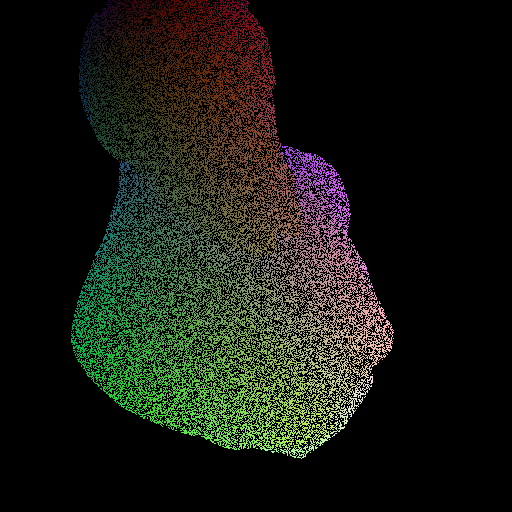
\includegraphics[width=.15\textwidth]{./Figures/train-input.png}};
		\node[text width=3.5cm] at (\vdist*\disttimes+1,\yschift-1.5) {3D Vertex};
		
		\draw [-stealth](1.45,\yschift-1.8) -- (1.45,\yschift-2.6);
		
		\draw [-stealth]  (\vdist*\disttimes+1.6,\yschift) -- (\vdist*\disttimes+1.1,\yschift);
		
		\pgfmathsetmacro{\disttimes}{10}
		\pgfmathsetmacro{\yschift}{\preprocessingshift}
		\node[inner sep=0pt] (depthmap) at (\vdist*\disttimes,\yschift)
		{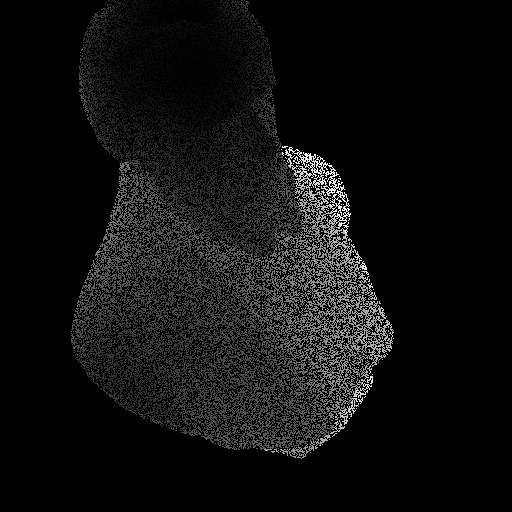
\includegraphics[width=.15\textwidth]{./Figures/train-depth-noise.png}};
		\node[text width=3.5cm] at (\vdist*\disttimes+1,\yschift-1.5) {Add Noise};
		
		\draw [-stealth] (\vdist*\disttimes+1.6,\yschift) -- (\vdist*\disttimes+1.1,\yschift);
		
		\pgfmathsetmacro{\disttimes}{16.5}
		\pgfmathsetmacro{\yschift}{\preprocessingshift}
		\node[inner sep=0pt] (depthmap) at (\vdist*\disttimes,\yschift)
		{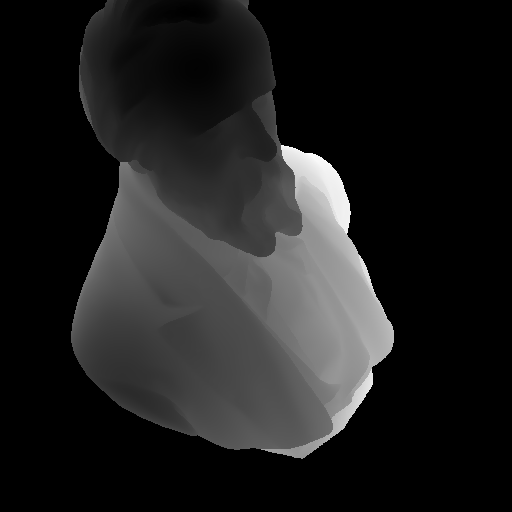
\includegraphics[width=.15\textwidth]{./Figures/train-depth.png}};
		\node[text width=2cm] at (\vdist*\disttimes+0.2,\yschift-1.5) {Depth Map};
		
		%% ------------------------------------ img preprocessing -------------------------------------
		\pgfmathsetmacro{\disttimes}{3.5}
		\pgfmathsetmacro{\yschift}{\imgshift}
		\node[inner sep=0pt] (image) at (\vdist*\disttimes,\yschift)
		{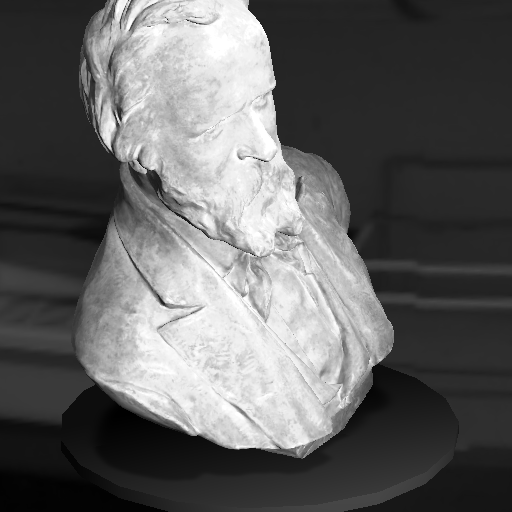
\includegraphics[width=.15\textwidth]{./Figures/train-image.png}};
		\node[text width=3.5cm] at (\vdist*\disttimes+1,\yschift-1.5) {Image};
		
		\draw [-stealth](1.45,\yschift-1.8) -- (1.45,\yschift-2.2);
		
		
		
		%% ----------------------------------- output normal map -------------------------------------
		\pgfmathsetmacro{\disttimes}{32.5}
		\pgfmathsetmacro{\yschift}{\preprocessingshift}
		\node[inner sep=0pt] (depthmap) at (\vdist*\disttimes,\yschift)
		{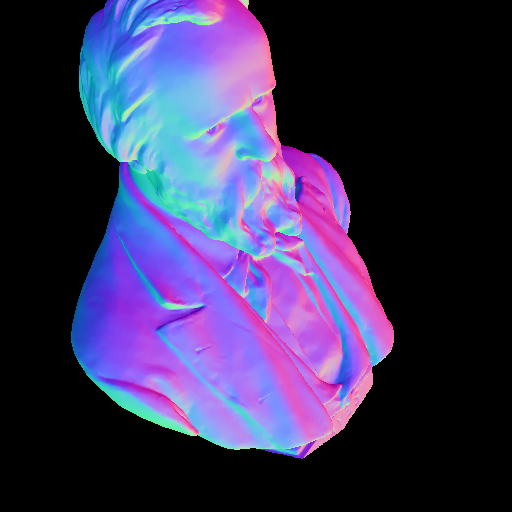
\includegraphics[width=.15\textwidth]{./Figures/train-normal-gt.png}};
		\node[text width=2.5cm] at (\vdist*\disttimes,\yschift-1.5) {Normal Map};
		
		\draw [-stealth] (\vdist*\disttimes+0.2,\yschift-2.7) -- (\vdist*\disttimes+0.2,\yschift-1.8);
		
		
		%% ------------------------------------------- vertex input ----------------------------------------------
		%% 	d_in							3x512x512
		%%	dconv1: 	d_in-->x1 			32x512x512
		\pgfmathsetmacro{\disttimes}{1}	%% width 32
		\pgfmathsetmacro{\boxsize}{\boxsizea}	%% size 512
		\pgfmathsetmacro{\boxwidth}{\boxwidthb}	%% width 32
		\pgfmathsetmacro{\yschift}{\gconvwshift}
		\node[text width=1cm] at (\vdist*\disttimes+0.1,\yschift-3.5) {32};
		\draw[black, fill=gconvcolor] (\vdist*\disttimes,\yschift,0) -- ++(-\boxwidth,0,0) -- ++(0,-\boxsize,0) -- ++(\boxwidth,0,0) -- cycle;
		\draw[black, fill=gconvcolor] (\vdist*\disttimes,\yschift,0) -- ++(0,0,-\boxsize) -- ++(0,-\boxsize,0) -- ++(0,0,\boxsize) -- cycle;
		\draw[black, fill=gconvcolor] (\vdist*\disttimes,\yschift,0) -- ++(-\boxwidth,0,0) -- ++(0,0,-\boxsize) -- ++(\boxwidth,0,0) -- cycle;
		
		%%	dconv2:		x1-->x1				32x512x512
		\pgfmathsetmacro{\disttimes}{2}	%% width 32
		\pgfmathsetmacro{\boxsize}{\boxsizea}	%% size 512
		\pgfmathsetmacro{\boxwidth}{\boxwidthb}	%% width 32
		\pgfmathsetmacro{\yschift}{\gconvwshift}
		\draw[black, fill=gconvcolor] (\vdist*\disttimes,\yschift,0) -- ++(-\boxwidth,0,0) -- ++(0,-\boxsize,0) -- ++(\boxwidth,0,0) -- cycle;
		\draw[black, fill=gconvcolor] (\vdist*\disttimes,\yschift,0) -- ++(0,0,-\boxsize) -- ++(0,-\boxsize,0) -- ++(0,0,\boxsize) -- cycle;
		\draw[black, fill=gconvcolor] (\vdist*\disttimes,\yschift,0) -- ++(-\boxwidth,0,0) -- ++(0,0,-\boxsize) -- ++(\boxwidth,0,0) -- cycle;
		
		%%	dconv3:		x1-->x1				32x512x512
		\pgfmathsetmacro{\disttimes}{3}	%% width 32
		\pgfmathsetmacro{\boxsize}{\boxsizea}	%% size 512
		\pgfmathsetmacro{\boxwidth}{\boxwidthb}	%% width 32
		\pgfmathsetmacro{\yschift}{\gconvwshift}
		\draw[black, fill=gconvcolor] (\vdist*\disttimes,\yschift,0) -- ++(-\boxwidth,0,0) -- ++(0,-\boxsize,0) -- ++(\boxwidth,0,0) -- cycle;
		\draw[black, fill=gconvcolor] (\vdist*\disttimes,\yschift,0) -- ++(0,0,-\boxsize) -- ++(0,-\boxsize,0) -- ++(0,0,\boxsize) -- cycle;
		\draw[black, fill=gconvcolor] (\vdist*\disttimes,\yschift,0) -- ++(-\boxwidth,0,0) -- ++(0,0,-\boxsize) -- ++(\boxwidth,0,0) -- cycle;
		
		\draw (\vdist*\disttimes-0.1,\yschift-3) -- (\vdist*\disttimes-0.1,\yschift-3.7);
		\draw (\vdist*\disttimes-0.1,\yschift-3.7) -- (\vdist*\disttimes+9.2,\yschift-3.7);
		\draw [-stealth] (\vdist*\disttimes+9.2,\yschift-3.7) -- (\vdist*\disttimes+9.2,\yschift-3);
		
		%% downsample 1
		%%	dconv4:		x1-->x2				32x256x256
		\pgfmathsetmacro{\disttimes}{4}	%% width 32
		\pgfmathsetmacro{\boxsize}{\boxsizeb}	%% size 256
		\pgfmathsetmacro{\boxwidth}{\boxwidthb}	%% width 32
		\pgfmathsetmacro{\yschift}{\gconvwshift-0.5}	%% width 32
		\draw[black, fill=gconvcolor] (\vdist*\disttimes,\yschift,0) -- ++(-\boxwidth,0,0) -- ++(0,-\boxsize,0) -- ++(\boxwidth,0,0) -- cycle;
		\draw[black, fill=gconvcolor] (\vdist*\disttimes,\yschift,0) -- ++(0,0,-\boxsize) -- ++(0,-\boxsize,0) -- ++(0,0,\boxsize) -- cycle;
		\draw[black, fill=gconvcolor] (\vdist*\disttimes,\yschift,0) -- ++(-\boxwidth,0,0) -- ++(0,0,-\boxsize) -- ++(\boxwidth,0,0) -- cycle;
		%%	dconv2:		x2-->x2				32x256x256
		\pgfmathsetmacro{\disttimes}{5}	%% width 32
		\pgfmathsetmacro{\boxsize}{\boxsizeb}	%% size 256
		\pgfmathsetmacro{\boxwidth}{\boxwidthb}	%% width 32
		\pgfmathsetmacro{\yschift}{\gconvwshift-0.5}	%% width 32
		\draw[black, fill=gconvcolor] (\vdist*\disttimes,\yschift,0) -- ++(-\boxwidth,0,0) -- ++(0,-\boxsize,0) -- ++(\boxwidth,0,0) -- cycle;
		\draw[black, fill=gconvcolor] (\vdist*\disttimes,\yschift,0) -- ++(0,0,-\boxsize) -- ++(0,-\boxsize,0) -- ++(0,0,\boxsize) -- cycle;
		\draw[black, fill=gconvcolor] (\vdist*\disttimes,\yschift,0) -- ++(-\boxwidth,0,0) -- ++(0,0,-\boxsize) -- ++(\boxwidth,0,0) -- cycle;
		%%	dconv3:		x2-->x2				32x256x256
		\pgfmathsetmacro{\disttimes}{6}	%% width 32
		\pgfmathsetmacro{\boxsize}{\boxsizeb}	%% size 256
		\pgfmathsetmacro{\boxwidth}{\boxwidthb}	%% width 32
		\pgfmathsetmacro{\yschift}{\gconvwshift-0.5}	%% width 32
		\draw[black, fill=gconvcolor] (\vdist*\disttimes,\yschift,0) -- ++(-\boxwidth,0,0) -- ++(0,-\boxsize,0) -- ++(\boxwidth,0,0) -- cycle;
		\draw[black, fill=gconvcolor] (\vdist*\disttimes,\yschift,0) -- ++(0,0,-\boxsize) -- ++(0,-\boxsize,0) -- ++(0,0,\boxsize) -- cycle;
		\draw[black, fill=gconvcolor] (\vdist*\disttimes,\yschift,0) -- ++(-\boxwidth,0,0) -- ++(0,0,-\boxsize) -- ++(\boxwidth,0,0) -- cycle;
		
		\draw (\vdist*\disttimes-0.1,\yschift-1.6) -- (\vdist*\disttimes-0.1,\yschift-2.7);
		\draw (\vdist*\disttimes-0.1,\yschift-2.7) -- (\vdist*\disttimes+6,\yschift-2.7);
		\draw [-stealth] (\vdist*\disttimes+6,\yschift-2.7) -- (\vdist*\disttimes+6,\yschift-1.7);
		
		
		%% downsample 2
		%%	dconv4:		x2-->x3				32x128x128
		\pgfmathsetmacro{\disttimes}{7}	%% width 32
		\pgfmathsetmacro{\boxsize}{\boxsizec}	%% size 128
		\pgfmathsetmacro{\boxwidth}{\boxwidthb}	%% width 32
		\pgfmathsetmacro{\yschift}{\gconvwshift-0.8}	%% width 32
		\draw[black, fill=gconvcolor] (\vdist*\disttimes,\yschift,0) -- ++(-\boxwidth,0,0) -- ++(0,-\boxsize,0) -- ++(\boxwidth,0,0) -- cycle;
		\draw[black, fill=gconvcolor] (\vdist*\disttimes,\yschift,0) -- ++(0,0,-\boxsize) -- ++(0,-\boxsize,0) -- ++(0,0,\boxsize) -- cycle;
		\draw[black, fill=gconvcolor] (\vdist*\disttimes,\yschift,0) -- ++(-\boxwidth,0,0) -- ++(0,0,-\boxsize) -- ++(\boxwidth,0,0) -- cycle;
		%%	dconv2:		x3-->x3				32x128x128
		\pgfmathsetmacro{\disttimes}{8}	%% width 32
		\pgfmathsetmacro{\boxsize}{\boxsizec}	%% size 128
		\pgfmathsetmacro{\boxwidth}{\boxwidthb}	%% width 32
		\pgfmathsetmacro{\yschift}{\gconvwshift-0.8}	%% width 32
		\draw[black, fill=gconvcolor] (\vdist*\disttimes,\yschift,0) -- ++(-\boxwidth,0,0) -- ++(0,-\boxsize,0) -- ++(\boxwidth,0,0) -- cycle;
		\draw[black, fill=gconvcolor] (\vdist*\disttimes,\yschift,0) -- ++(0,0,-\boxsize) -- ++(0,-\boxsize,0) -- ++(0,0,\boxsize) -- cycle;
		\draw[black, fill=gconvcolor] (\vdist*\disttimes,\yschift,0) -- ++(-\boxwidth,0,0) -- ++(0,0,-\boxsize) -- ++(\boxwidth,0,0) -- cycle;
		%%	dconv3:		x3-->x3				32x128x128
		\pgfmathsetmacro{\disttimes}{9}	%% width 32
		\pgfmathsetmacro{\boxsize}{\boxsizec}	%% size 128
		\pgfmathsetmacro{\boxwidth}{\boxwidthb}	%% width 32
		\pgfmathsetmacro{\yschift}{\gconvwshift-0.8}	%% width 32
		\draw[black, fill=gconvcolor] (\vdist*\disttimes,\yschift,0) -- ++(-\boxwidth,0,0) -- ++(0,-\boxsize,0) -- ++(\boxwidth,0,0) -- cycle;
		\draw[black, fill=gconvcolor] (\vdist*\disttimes,\yschift,0) -- ++(0,0,-\boxsize) -- ++(0,-\boxsize,0) -- ++(0,0,\boxsize) -- cycle;
		\draw[black, fill=gconvcolor] (\vdist*\disttimes,\yschift,0) -- ++(-\boxwidth,0,0) -- ++(0,0,-\boxsize) -- ++(\boxwidth,0,0) -- cycle;
		
		\draw (\vdist*\disttimes-0.1,\yschift-1.2) -- (\vdist*\disttimes-0.1,\yschift-1.8);
		\draw (\vdist*\disttimes-0.1,\yschift-1.8) -- (\vdist*\disttimes+2.8,\yschift-1.8);
		\draw [-stealth] (\vdist*\disttimes+2.8,\yschift-1.8) -- (\vdist*\disttimes+2.8,\yschift-1.2);
		
		
		%% downsample 3
		%%	dconv4:		x3-->x4				32x64x64
		\pgfmathsetmacro{\disttimes}{10}
		\pgfmathsetmacro{\boxsize}{\boxsized}	%% size 64
		\pgfmathsetmacro{\boxwidth}{\boxwidthb}	%% width 32
		\pgfmathsetmacro{\yschift}{\gconvwshift-1}
		\draw[black, fill=gconvcolor] (\vdist*\disttimes,\yschift,0) -- ++(-\boxwidth,0,0) -- ++(0,-\boxsize,0) -- ++(\boxwidth,0,0) -- cycle;
		\draw[black, fill=gconvcolor] (\vdist*\disttimes,\yschift,0) -- ++(0,0,-\boxsize) -- ++(0,-\boxsize,0) -- ++(0,0,\boxsize) -- cycle;
		\draw[black, fill=gconvcolor] (\vdist*\disttimes,\yschift,0) -- ++(-\boxwidth,0,0) -- ++(0,0,-\boxsize) -- ++(\boxwidth,0,0) -- cycle;
		%%	dconv2:		x4-->x4				32x64x64
		\pgfmathsetmacro{\disttimes}{11}
		\pgfmathsetmacro{\boxsize}{\boxsized}	%% size 64
		\pgfmathsetmacro{\boxwidth}{\boxwidthb}	%% width 32
		\pgfmathsetmacro{\yschift}{\gconvwshift-1}	%% width 32
		\draw[black, fill=gconvcolor] (\vdist*\disttimes,\yschift,0) -- ++(-\boxwidth,0,0) -- ++(0,-\boxsize,0) -- ++(\boxwidth,0,0) -- cycle;
		\draw[black, fill=gconvcolor] (\vdist*\disttimes,\yschift,0) -- ++(0,0,-\boxsize) -- ++(0,-\boxsize,0) -- ++(0,0,\boxsize) -- cycle;
		\draw[black, fill=gconvcolor] (\vdist*\disttimes,\yschift,0) -- ++(-\boxwidth,0,0) -- ++(0,0,-\boxsize) -- ++(\boxwidth,0,0) -- cycle;
		%%	dconv3:		x4-->x4				32x64x64
		\pgfmathsetmacro{\disttimes}{12}
		\pgfmathsetmacro{\boxsize}{\boxsized}	%% size 64
		\pgfmathsetmacro{\boxwidth}{\boxwidthb}	%% width 32
		\pgfmathsetmacro{\yschift}{\gconvwshift-1}	%% width 32
		\draw[black, fill=gconvcolor] (\vdist*\disttimes,\yschift,0) -- ++(-\boxwidth,0,0) -- ++(0,-\boxsize,0) -- ++(\boxwidth,0,0) -- cycle;
		\draw[black, fill=gconvcolor] (\vdist*\disttimes,\yschift,0) -- ++(0,0,-\boxsize) -- ++(0,-\boxsize,0) -- ++(0,0,\boxsize) -- cycle;
		\draw[black, fill=gconvcolor] (\vdist*\disttimes,\yschift,0) -- ++(-\boxwidth,0,0) -- ++(0,0,-\boxsize) -- ++(\boxwidth,0,0) -- cycle;
		
		
		%% concatenated x4 and x_img_4
		\pgfmathsetmacro{\disttimes}{13}
		\pgfmathsetmacro{\boxsize}{\boxsized}	%% size 64
		\pgfmathsetmacro{\boxwidth}{\boxwidthc}	%% width 32
		\pgfmathsetmacro{\yschift}{\gconvwshift-1}	%% width 32
		\draw[black, fill=catcolor] (\vdist*\disttimes,\yschift,0) -- ++(-\boxwidth,0,0) -- ++(0,-\boxsize,0) -- ++(\boxwidth,0,0) -- cycle;
		\draw[black, fill=catcolor] (\vdist*\disttimes,\yschift,0) -- ++(0,0,-\boxsize) -- ++(0,-\boxsize,0) -- ++(0,0,\boxsize) -- cycle;
		\draw[black, fill=catcolor] (\vdist*\disttimes,\yschift,0) -- ++(-\boxwidth,0,0) -- ++(0,0,-\boxsize) -- ++(\boxwidth,0,0) -- cycle;
		
		
		%% ----------------------------------- upsampling -------------------------------------
		
		%% upsample 1
		%% interpolate	x3_us-->x3_mus			64x128x128
		\pgfmathsetmacro{\disttimes}{14}
		\pgfmathsetmacro{\boxsize}{\boxsizec}	%% size 128
		\pgfmathsetmacro{\boxwidth}{\boxwidthc}	%% width 32
		\pgfmathsetmacro{\yschift}{\gconvwshift-0.9}	%% width 32
		\draw[black, fill=interpolatecolor] (\vdist*\disttimes,\yschift,0) -- ++(-\boxwidth,0,0) -- ++(0,-\boxsize,0) -- ++(\boxwidth,0,0) -- cycle;
		\draw[black, fill=interpolatecolor] (\vdist*\disttimes,\yschift,0) -- ++(0,0,-\boxsize) -- ++(0,-\boxsize,0) -- ++(0,0,\boxsize) -- cycle;
		\draw[black, fill=interpolatecolor] (\vdist*\disttimes,\yschift,0) -- ++(-\boxwidth,0,0) -- ++(0,0,-\boxsize) -- ++(\boxwidth,0,0) -- cycle;
		
		% uconv 1
		\pgfmathsetmacro{\disttimes}{15}
		\pgfmathsetmacro{\boxsize}{\boxsizec}	%% size 128
		\pgfmathsetmacro{\boxwidth}{\boxwidthb}	%% width 32
		\pgfmathsetmacro{\yschift}{\gconvwshift-0.9}	%% width 32
		\draw[black, fill=gconvcolor] (\vdist*\disttimes,\yschift,0) -- ++(-\boxwidth,0,0) -- ++(0,-\boxsize,0) -- ++(\boxwidth,0,0) -- cycle;
		\draw[black, fill=gconvcolor] (\vdist*\disttimes,\yschift,0) -- ++(0,0,-\boxsize) -- ++(0,-\boxsize,0) -- ++(0,0,\boxsize) -- cycle;
		\draw[black, fill=gconvcolor] (\vdist*\disttimes,\yschift,0) -- ++(-\boxwidth,0,0) -- ++(0,0,-\boxsize) -- ++(\boxwidth,0,0) -- cycle;
		
		
		%% concatenated x1 and x1_us
		\pgfmathsetmacro{\disttimes}{15.5}
		\pgfmathsetmacro{\boxsize}{\boxsizec}	%% size 512
		\pgfmathsetmacro{\boxwidth}{\boxwidthc}	%% width 32
		\pgfmathsetmacro{\yschift}{\gconvwshift-0.9}	%% width 32
		\draw[black, fill=catcolor] (\vdist*\disttimes+\boxwidth,\yschift,0) -- ++(-\boxwidth,0,0) -- ++(0,-\boxsize,0) -- ++(\boxwidth,0,0) -- cycle;
		\draw[black, fill=catcolor] (\vdist*\disttimes+\boxwidth,\yschift,0) -- ++(0,0,-\boxsize) -- ++(0,-\boxsize,0) -- ++(0,0,\boxsize) -- cycle;
		\draw[black, fill=catcolor] (\vdist*\disttimes+\boxwidth,\yschift,0) -- ++(-\boxwidth,0,0) -- ++(0,0,-\boxsize) -- ++(\boxwidth,0,0) -- cycle;
		
		%% uconv2		x3_us-->x3			32x128x128
		\pgfmathsetmacro{\disttimes}{17}
		\pgfmathsetmacro{\boxsize}{\boxsizec}	%% size 128
		\pgfmathsetmacro{\boxwidth}{\boxwidthb}	%% width 32
		\pgfmathsetmacro{\yschift}{\gconvwshift-0.9}	%% width 32
		\draw[black, fill=gconvcolor] (\vdist*\disttimes,\yschift,0) -- ++(-\boxwidth,0,0) -- ++(0,-\boxsize,0) -- ++(\boxwidth,0,0) -- cycle;
		\draw[black, fill=gconvcolor] (\vdist*\disttimes,\yschift,0) -- ++(0,0,-\boxsize) -- ++(0,-\boxsize,0) -- ++(0,0,\boxsize) -- cycle;
		\draw[black, fill=gconvcolor] (\vdist*\disttimes,\yschift,0) -- ++(-\boxwidth,0,0) -- ++(0,0,-\boxsize) -- ++(\boxwidth,0,0) -- cycle;
		
		%% upsample 2
		%% cat x3, x_img_3-->x3			64x256x256
		\pgfmathsetmacro{\disttimes}{18}
		\pgfmathsetmacro{\boxsize}{\boxsizec}	%% size 256
		\pgfmathsetmacro{\boxwidth}{\boxwidthc}	%% width 32
		\pgfmathsetmacro{\yschift}{\gconvwshift-0.9}	%% width 32
		\draw[black, fill=catcolor] (\vdist*\disttimes,\yschift,0) -- ++(-\boxwidth,0,0) -- ++(0,-\boxsize,0) -- ++(\boxwidth,0,0) -- cycle;
		\draw[black, fill=catcolor] (\vdist*\disttimes,\yschift,0) -- ++(0,0,-\boxsize) -- ++(0,-\boxsize,0) -- ++(0,0,\boxsize) -- cycle;
		\draw[black, fill=catcolor] (\vdist*\disttimes,\yschift,0) -- ++(-\boxwidth,0,0) -- ++(0,0,-\boxsize) -- ++(\boxwidth,0,0) -- cycle;
		
		´%% interpolate x2_us 64x256x256
		\pgfmathsetmacro{\disttimes}{18.5}
		\pgfmathsetmacro{\boxsize}{\boxsizeb}	%% size 256
		\pgfmathsetmacro{\boxwidth}{\boxwidthc}	%% width 32
		\pgfmathsetmacro{\yschift}{\gconvwshift-0.6}	%% width 32
		\draw[black, fill=interpolatecolor] (\vdist*\disttimes,\yschift,0) -- ++(-\boxwidth,0,0) -- ++(0,-\boxsize,0) -- ++(\boxwidth,0,0) -- cycle;
		\draw[black, fill=interpolatecolor] (\vdist*\disttimes,\yschift,0) -- ++(0,0,-\boxsize) -- ++(0,-\boxsize,0) -- ++(0,0,\boxsize) -- cycle;
		\draw[black, fill=interpolatecolor] (\vdist*\disttimes,\yschift,0) -- ++(-\boxwidth,0,0) -- ++(0,0,-\boxsize) -- ++(\boxwidth,0,0) -- cycle;		
		
		%% uconv3 x2_us -->x2_mus
		\pgfmathsetmacro{\disttimes}{19}
		\pgfmathsetmacro{\boxsize}{\boxsizeb}	%% size 256
		\pgfmathsetmacro{\boxwidth}{\boxwidthb}	%% width 32
		\pgfmathsetmacro{\yschift}{\gconvwshift-0.6}	%% width 32
		\draw[black, fill=gconvcolor] (\vdist*\disttimes+\boxwidth,\yschift,0) -- ++(-\boxwidth,0,0) -- ++(0,-\boxsize,0) -- ++(\boxwidth,0,0) -- cycle;
		\draw[black, fill=gconvcolor] (\vdist*\disttimes+\boxwidth,\yschift,0) -- ++(0,0,-\boxsize) -- ++(0,-\boxsize,0) -- ++(0,0,\boxsize) -- cycle;
		\draw[black, fill=gconvcolor] (\vdist*\disttimes+\boxwidth,\yschift,0) -- ++(-\boxwidth,0,0) -- ++(0,0,-\boxsize) -- ++(\boxwidth,0,0) -- cycle;
		
		% cat x2, x2_mus -->x2
		\pgfmathsetmacro{\disttimes}{20}
		\pgfmathsetmacro{\boxsize}{\boxsizeb}	%% size 256
		\pgfmathsetmacro{\boxwidth}{\boxwidthc}	%% width 32
		\pgfmathsetmacro{\yschift}{\gconvwshift-0.6}	%% width 32
		\draw[black, fill=catcolor] (\vdist*\disttimes+\boxwidth,\yschift,0) -- ++(-\boxwidth,0,0) -- ++(0,-\boxsize,0) -- ++(\boxwidth,0,0) -- cycle;
		\draw[black, fill=catcolor] (\vdist*\disttimes+\boxwidth,\yschift,0) -- ++(0,0,-\boxsize) -- ++(0,-\boxsize,0) -- ++(0,0,\boxsize) -- cycle;
		\draw[black, fill=catcolor] (\vdist*\disttimes+\boxwidth,\yschift,0) -- ++(-\boxwidth,0,0) -- ++(0,0,-\boxsize) -- ++(\boxwidth,0,0) -- cycle;
		
		%% uconv4 		x2,x2_us-->x2		32x256x256
		\pgfmathsetmacro{\disttimes}{21.5}
		\pgfmathsetmacro{\boxsize}{\boxsizeb}	%% size 256
		\pgfmathsetmacro{\boxwidth}{\boxwidthb}	%% width 32
		\pgfmathsetmacro{\yschift}{\gconvwshift-0.6}	%% width 32
		\draw[black, fill=gconvcolor] (\vdist*\disttimes,\yschift,0) -- ++(-\boxwidth,0,0) -- ++(0,-\boxsize,0) -- ++(\boxwidth,0,0) -- cycle;
		\draw[black, fill=gconvcolor] (\vdist*\disttimes,\yschift,0) -- ++(0,0,-\boxsize) -- ++(0,-\boxsize,0) -- ++(0,0,\boxsize) -- cycle;
		\draw[black, fill=gconvcolor] (\vdist*\disttimes,\yschift,0) -- ++(-\boxwidth,0,0) -- ++(0,0,-\boxsize) -- ++(\boxwidth,0,0) -- cycle;
		
		
		%% upsample 3
		%% cat x2, x_img_2-->x2			64x256x256
		\pgfmathsetmacro{\disttimes}{22.5}
		\pgfmathsetmacro{\boxsize}{\boxsizeb}	%% size 256
		\pgfmathsetmacro{\boxwidth}{\boxwidthc}	%% width 32
		\pgfmathsetmacro{\yschift}{\gconvwshift-0.6}	%% width 32
		\draw[black, fill=catcolor] (\vdist*\disttimes,\yschift,0) -- ++(-\boxwidth,0,0) -- ++(0,-\boxsize,0) -- ++(\boxwidth,0,0) -- cycle;
		\draw[black, fill=catcolor] (\vdist*\disttimes,\yschift,0) -- ++(0,0,-\boxsize) -- ++(0,-\boxsize,0) -- ++(0,0,\boxsize) -- cycle;
		\draw[black, fill=catcolor] (\vdist*\disttimes,\yschift,0) -- ++(-\boxwidth,0,0) -- ++(0,0,-\boxsize) -- ++(\boxwidth,0,0) -- cycle;
		
		%% interpolate	x2-->x1_us			32x512x512
		\pgfmathsetmacro{\disttimes}{23.5}
		\pgfmathsetmacro{\boxsize}{\boxsizea}	%% size 512
		\pgfmathsetmacro{\boxwidth}{\boxwidthc}	%% width 32
		\pgfmathsetmacro{\yschift}{\gconvwshift}	%% width 32
		\draw[black, fill=interpolatecolor] (\vdist*\disttimes,\yschift,0) -- ++(-\boxwidth,0,0) -- ++(0,-\boxsize,0) -- ++(\boxwidth,0,0) -- cycle;
		\draw[black, fill=interpolatecolor] (\vdist*\disttimes,\yschift,0) -- ++(0,0,-\boxsize) -- ++(0,-\boxsize,0) -- ++(0,0,\boxsize) -- cycle;
		\draw[black, fill=interpolatecolor] (\vdist*\disttimes,\yschift,0) -- ++(-\boxwidth,0,0) -- ++(0,0,-\boxsize) -- ++(\boxwidth,0,0) -- cycle;
		
		%% uconv5 x1_us-->x1_mus
		\pgfmathsetmacro{\disttimes}{24}
		\pgfmathsetmacro{\boxsize}{\boxsizea}	%% size 256
		\pgfmathsetmacro{\boxwidth}{\boxwidthb}	%% width 32
		\pgfmathsetmacro{\yschift}{\gconvwshift}	%% width 32
		\draw[black, fill=gconvcolor] (\vdist*\disttimes+\boxwidth,\yschift,0) -- ++(-\boxwidth,0,0) -- ++(0,-\boxsize,0) -- ++(\boxwidth,0,0) -- cycle;
		\draw[black, fill=gconvcolor] (\vdist*\disttimes+\boxwidth,\yschift,0) -- ++(0,0,-\boxsize) -- ++(0,-\boxsize,0) -- ++(0,0,\boxsize) -- cycle;
		\draw[black, fill=gconvcolor] (\vdist*\disttimes+\boxwidth,\yschift,0) -- ++(-\boxwidth,0,0) -- ++(0,0,-\boxsize) -- ++(\boxwidth,0,0) -- cycle;
		
		
		%% cat		x1,x1_mus-->x1		32x512x512
		\pgfmathsetmacro{\disttimes}{26}
		\pgfmathsetmacro{\boxsize}{\boxsizea}	%% size 512
		\pgfmathsetmacro{\boxwidth}{\boxwidthc}	%% width 32
		\pgfmathsetmacro{\yschift}{\gconvwshift}	%% width 32
		\draw[black, fill=catcolor] (\vdist*\disttimes,\yschift,0) -- ++(-\boxwidth,0,0) -- ++(0,-\boxsize,0) -- ++(\boxwidth,0,0) -- cycle;
		\draw[black, fill=catcolor] (\vdist*\disttimes,\yschift,0) -- ++(0,0,-\boxsize) -- ++(0,-\boxsize,0) -- ++(0,0,\boxsize) -- cycle;
		\draw[black, fill=catcolor] (\vdist*\disttimes,\yschift,0) -- ++(-\boxwidth,0,0) -- ++(0,0,-\boxsize) -- ++(\boxwidth,0,0) -- cycle;
		
		%% uconv6		x1			32x512x512
		\pgfmathsetmacro{\disttimes}{27}
		\pgfmathsetmacro{\boxsize}{\boxsizea}	%% size 512
		\pgfmathsetmacro{\boxwidth}{\boxwidthb}	%% width 3
		\pgfmathsetmacro{\yschift}{\gconvwshift}	%% width 32
		\draw[black, fill=gconvcolor] (\vdist*\disttimes,\yschift,0) -- ++(-\boxwidth,0,0) -- ++(0,-\boxsize,0) -- ++(\boxwidth,0,0) -- cycle;
		\draw[black, fill=gconvcolor] (\vdist*\disttimes,\yschift,0) -- ++(0,0,-\boxsize) -- ++(0,-\boxsize,0) -- ++(0,0,\boxsize) -- cycle;
		\draw[black, fill=gconvcolor] (\vdist*\disttimes,\yschift,0) -- ++(-\boxwidth,0,0) -- ++(0,0,-\boxsize) -- ++(\boxwidth,0,0) -- cycle;
		
		%% cat		x1,x1_mus-->x1		32x512x512
		\pgfmathsetmacro{\disttimes}{28}
		\pgfmathsetmacro{\boxsize}{\boxsizea}	%% size 512
		\pgfmathsetmacro{\boxwidth}{\boxwidthc}	%% width 32
		\pgfmathsetmacro{\yschift}{\gconvwshift}	%% width 32
		\draw[black, fill=catcolor] (\vdist*\disttimes,\yschift,0) -- ++(-\boxwidth,0,0) -- ++(0,-\boxsize,0) -- ++(\boxwidth,0,0) -- cycle;
		\draw[black, fill=catcolor] (\vdist*\disttimes,\yschift,0) -- ++(0,0,-\boxsize) -- ++(0,-\boxsize,0) -- ++(0,0,\boxsize) -- cycle;
		\draw[black, fill=catcolor] (\vdist*\disttimes,\yschift,0) -- ++(-\boxwidth,0,0) -- ++(0,0,-\boxsize) -- ++(\boxwidth,0,0) -- cycle;
		
		%% conv1		xout			3x512x512
		\pgfmathsetmacro{\disttimes}{29}
		\pgfmathsetmacro{\boxsize}{\boxsizea}	%% size 512
		\pgfmathsetmacro{\boxwidth}{\boxwidtha}	%% width 3
		\pgfmathsetmacro{\yschift}{\gconvwshift}	%% width 32
		\draw[black, fill=convcolor] (\vdist*\disttimes,\yschift,0) -- ++(-\boxwidth,0,0) -- ++(0,-\boxsize,0) -- ++(\boxwidth,0,0) -- cycle;
		\draw[black, fill=convcolor] (\vdist*\disttimes,\yschift,0) -- ++(0,0,-\boxsize) -- ++(0,-\boxsize,0) -- ++(0,0,\boxsize) -- cycle;
		\draw[black, fill=convcolor] (\vdist*\disttimes,\yschift,0) -- ++(-\boxwidth,0,0) -- ++(0,0,-\boxsize) -- ++(\boxwidth,0,0) -- cycle;
		%% conv2		xout			3x512x512
		\pgfmathsetmacro{\disttimes}{30}
		\pgfmathsetmacro{\boxsize}{\boxsizea}	%% size 512
		\pgfmathsetmacro{\boxwidth}{\boxwidtha}	%% width 3
		\pgfmathsetmacro{\yschift}{\gconvwshift}	%% width 32
		\node[text width=1cm] at (\vdist*\disttimes+0.3,\yschift-3.3) {3};
		\draw[black, fill=convcolor] (\vdist*\disttimes,\yschift,0) -- ++(-\boxwidth,0,0) -- ++(0,-\boxsize,0) -- ++(\boxwidth,0,0) -- cycle;
		\draw[black, fill=convcolor] (\vdist*\disttimes,\yschift,0) -- ++(0,0,-\boxsize) -- ++(0,-\boxsize,0) -- ++(0,0,\boxsize) -- cycle;
		\draw[black, fill=convcolor] (\vdist*\disttimes,\yschift,0) -- ++(-\boxwidth,0,0) -- ++(0,0,-\boxsize) -- ++(\boxwidth,0,0) -- cycle;
		
		% -------------------------- image branch ----------------------------------------------
		
		%% ------------------------------------------- image input ----------------------------------------------
		%% 	d_in							3x512x512
		%%	dconv1: 	d_in-->x1 			32x512x512
		\pgfmathsetmacro{\disttimes}{1}	%% width 32
		\pgfmathsetmacro{\boxsize}{\boxsizea}	%% size 512
		\pgfmathsetmacro{\boxwidth}{\boxwidthb}	%% width 32
		\pgfmathsetmacro{\yschift}{\convwshift}
		\node[text width=1cm] at (\vdist*\disttimes+0.1,\yschift-3.5) {32};
		\draw[black, fill=convcolor] (\vdist*\disttimes,\yschift,0) -- ++(-\boxwidth,0,0) -- ++(0,-\boxsize,0) -- ++(\boxwidth,0,0) -- cycle;
		\draw[black, fill=convcolor] (\vdist*\disttimes,\yschift,0) -- ++(0,0,-\boxsize) -- ++(0,-\boxsize,0) -- ++(0,0,\boxsize) -- cycle;
		\draw[black, fill=convcolor] (\vdist*\disttimes,\yschift,0) -- ++(-\boxwidth,0,0) -- ++(0,0,-\boxsize) -- ++(\boxwidth,0,0) -- cycle;
		
		%%	dconv2:		x1-->x1				32x512x512
		\pgfmathsetmacro{\disttimes}{2}	%% width 32
		\pgfmathsetmacro{\boxsize}{\boxsizea}	%% size 512
		\pgfmathsetmacro{\boxwidth}{\boxwidthb}	%% width 32
		\pgfmathsetmacro{\yschift}{\convwshift}
		\draw[black, fill=convcolor] (\vdist*\disttimes,\yschift,0) -- ++(-\boxwidth,0,0) -- ++(0,-\boxsize,0) -- ++(\boxwidth,0,0) -- cycle;
		\draw[black, fill=convcolor] (\vdist*\disttimes,\yschift,0) -- ++(0,0,-\boxsize) -- ++(0,-\boxsize,0) -- ++(0,0,\boxsize) -- cycle;
		\draw[black, fill=convcolor] (\vdist*\disttimes,\yschift,0) -- ++(-\boxwidth,0,0) -- ++(0,0,-\boxsize) -- ++(\boxwidth,0,0) -- cycle;
		
		%%	dconv3:		x1-->x1				32x512x512
		\pgfmathsetmacro{\disttimes}{3}	%% width 32
		\pgfmathsetmacro{\boxsize}{\boxsizea}	%% size 512
		\pgfmathsetmacro{\boxwidth}{\boxwidthb}	%% width 32
		\pgfmathsetmacro{\yschift}{\convwshift}
		\draw[black, fill=convcolor] (\vdist*\disttimes,\yschift,0) -- ++(-\boxwidth,0,0) -- ++(0,-\boxsize,0) -- ++(\boxwidth,0,0) -- cycle;
		\draw[black, fill=convcolor] (\vdist*\disttimes,\yschift,0) -- ++(0,0,-\boxsize) -- ++(0,-\boxsize,0) -- ++(0,0,\boxsize) -- cycle;
		\draw[black, fill=convcolor] (\vdist*\disttimes,\yschift,0) -- ++(-\boxwidth,0,0) -- ++(0,0,-\boxsize) -- ++(\boxwidth,0,0) -- cycle;
		
		\draw (\vdist*\disttimes-0.1,\yschift-3) -- (\vdist*\disttimes-0.1,\yschift-3.8);
		\draw (\vdist*\disttimes-0.1,\yschift-3.8) -- (\vdist*\disttimes+6.8,\yschift-3.8);
		\draw [-stealth] (\vdist*\disttimes+6.8,\yschift-3.8) -- (\vdist*\disttimes+6.8,\yschift-3);
		
		
		%% downsample 1
		%% dconv4:		x1-->x2				32x256x256
		\pgfmathsetmacro{\disttimes}{4}	%% width 32
		\pgfmathsetmacro{\boxsize}{\boxsizeb}	%% size 256
		\pgfmathsetmacro{\boxwidth}{\boxwidthb}	%% width 32
		\pgfmathsetmacro{\yschift}{\convwshift-0.5}	%% width 32
		\draw[black, fill=convcolor] (\vdist*\disttimes,\yschift,0) -- ++(-\boxwidth,0,0) -- ++(0,-\boxsize,0) -- ++(\boxwidth,0,0) -- cycle;
		\draw[black, fill=convcolor] (\vdist*\disttimes,\yschift,0) -- ++(0,0,-\boxsize) -- ++(0,-\boxsize,0) -- ++(0,0,\boxsize) -- cycle;
		\draw[black, fill=convcolor] (\vdist*\disttimes,\yschift,0) -- ++(-\boxwidth,0,0) -- ++(0,0,-\boxsize) -- ++(\boxwidth,0,0) -- cycle;
		%%	dconv2:		x2-->x2				32x256x256
		\pgfmathsetmacro{\disttimes}{5}	%% width 32
		\pgfmathsetmacro{\boxsize}{\boxsizeb}	%% size 256
		\pgfmathsetmacro{\boxwidth}{\boxwidthb}	%% width 32
		\pgfmathsetmacro{\yschift}{\convwshift-0.5}	%% width 32
		\draw[black, fill=convcolor] (\vdist*\disttimes,\yschift,0) -- ++(-\boxwidth,0,0) -- ++(0,-\boxsize,0) -- ++(\boxwidth,0,0) -- cycle;
		\draw[black, fill=convcolor] (\vdist*\disttimes,\yschift,0) -- ++(0,0,-\boxsize) -- ++(0,-\boxsize,0) -- ++(0,0,\boxsize) -- cycle;
		\draw[black, fill=convcolor] (\vdist*\disttimes,\yschift,0) -- ++(-\boxwidth,0,0) -- ++(0,0,-\boxsize) -- ++(\boxwidth,0,0) -- cycle;
		%%	dconv3:		x2-->x2				32x256x256
		\pgfmathsetmacro{\disttimes}{6}	%% width 32
		\pgfmathsetmacro{\boxsize}{\boxsizeb}	%% size 256
		\pgfmathsetmacro{\boxwidth}{\boxwidthb}	%% width 32
		\pgfmathsetmacro{\yschift}{\convwshift-0.5}	%% width 32
		\draw[black, fill=convcolor] (\vdist*\disttimes,\yschift,0) -- ++(-\boxwidth,0,0) -- ++(0,-\boxsize,0) -- ++(\boxwidth,0,0) -- cycle;
		\draw[black, fill=convcolor] (\vdist*\disttimes,\yschift,0) -- ++(0,0,-\boxsize) -- ++(0,-\boxsize,0) -- ++(0,0,\boxsize) -- cycle;
		\draw[black, fill=convcolor] (\vdist*\disttimes,\yschift,0) -- ++(-\boxwidth,0,0) -- ++(0,0,-\boxsize) -- ++(\boxwidth,0,0) -- cycle;
		
		
		\draw (\vdist*\disttimes-0.1,\yschift-1.5) -- (\vdist*\disttimes-0.1,\yschift-2.3);
		\draw (\vdist*\disttimes-0.1,\yschift-2.3) -- (\vdist*\disttimes+4.3,\yschift-2.3);
		\draw [-stealth] (\vdist*\disttimes+4.3,\yschift-2.3) -- (\vdist*\disttimes+4.3,\yschift-1.6);
		
		%% downsample 2
		%%	dconv4:		x2-->x3				32x128x128
		\pgfmathsetmacro{\disttimes}{7}	%% width 32
		\pgfmathsetmacro{\boxsize}{\boxsizec}	%% size 128
		\pgfmathsetmacro{\boxwidth}{\boxwidthb}	%% width 32
		\pgfmathsetmacro{\yschift}{\convwshift-0.8}	%% width 32
		\draw[black, fill=convcolor] (\vdist*\disttimes,\yschift,0) -- ++(-\boxwidth,0,0) -- ++(0,-\boxsize,0) -- ++(\boxwidth,0,0) -- cycle;
		\draw[black, fill=convcolor] (\vdist*\disttimes,\yschift,0) -- ++(0,0,-\boxsize) -- ++(0,-\boxsize,0) -- ++(0,0,\boxsize) -- cycle;
		\draw[black, fill=convcolor] (\vdist*\disttimes,\yschift,0) -- ++(-\boxwidth,0,0) -- ++(0,0,-\boxsize) -- ++(\boxwidth,0,0) -- cycle;
		%%	dconv2:		x3-->x3				32x128x128
		\pgfmathsetmacro{\disttimes}{8}	%% width 32
		\pgfmathsetmacro{\boxsize}{\boxsizec}	%% size 128
		\pgfmathsetmacro{\boxwidth}{\boxwidthb}	%% width 32
		\pgfmathsetmacro{\yschift}{\convwshift-0.8}	%% width 32
		\draw[black, fill=convcolor] (\vdist*\disttimes,\yschift,0) -- ++(-\boxwidth,0,0) -- ++(0,-\boxsize,0) -- ++(\boxwidth,0,0) -- cycle;
		\draw[black, fill=convcolor] (\vdist*\disttimes,\yschift,0) -- ++(0,0,-\boxsize) -- ++(0,-\boxsize,0) -- ++(0,0,\boxsize) -- cycle;
		\draw[black, fill=convcolor] (\vdist*\disttimes,\yschift,0) -- ++(-\boxwidth,0,0) -- ++(0,0,-\boxsize) -- ++(\boxwidth,0,0) -- cycle;
		%%	dconv3:		x3-->x3				32x128x128
		\pgfmathsetmacro{\disttimes}{9}	%% width 32
		\pgfmathsetmacro{\boxsize}{\boxsizec}	%% size 128
		\pgfmathsetmacro{\boxwidth}{\boxwidthb}	%% width 32
		\pgfmathsetmacro{\yschift}{\convwshift-0.8}	%% width 32
		\draw[black, fill=convcolor] (\vdist*\disttimes,\yschift,0) -- ++(-\boxwidth,0,0) -- ++(0,-\boxsize,0) -- ++(\boxwidth,0,0) -- cycle;
		\draw[black, fill=convcolor] (\vdist*\disttimes,\yschift,0) -- ++(0,0,-\boxsize) -- ++(0,-\boxsize,0) -- ++(0,0,\boxsize) -- cycle;
		\draw[black, fill=convcolor] (\vdist*\disttimes,\yschift,0) -- ++(-\boxwidth,0,0) -- ++(0,0,-\boxsize) -- ++(\boxwidth,0,0) -- cycle;
		
		
		\draw (\vdist*\disttimes-0.1,\yschift-1) -- (\vdist*\disttimes-0.1,\yschift-1.5);
		\draw (\vdist*\disttimes-0.1,\yschift-1.5) -- (\vdist*\disttimes+1.8,\yschift-1.5);
		\draw [-stealth] (\vdist*\disttimes+1.8,\yschift-1.5) -- (\vdist*\disttimes+1.8,\yschift-1.1);
		
		
		%% downsample 3
		%%	dconv4:		x3-->x4				32x64x64
		\pgfmathsetmacro{\disttimes}{10}
		\pgfmathsetmacro{\boxsize}{\boxsized}	%% size 64
		\pgfmathsetmacro{\boxwidth}{\boxwidthb}	%% width 32
		\pgfmathsetmacro{\yschift}{\convwshift-1}
		\draw[black, fill=convcolor] (\vdist*\disttimes,\yschift,0) -- ++(-\boxwidth,0,0) -- ++(0,-\boxsize,0) -- ++(\boxwidth,0,0) -- cycle;
		\draw[black, fill=convcolor] (\vdist*\disttimes,\yschift,0) -- ++(0,0,-\boxsize) -- ++(0,-\boxsize,0) -- ++(0,0,\boxsize) -- cycle;
		\draw[black, fill=convcolor] (\vdist*\disttimes,\yschift,0) -- ++(-\boxwidth,0,0) -- ++(0,0,-\boxsize) -- ++(\boxwidth,0,0) -- cycle;
		%%	dconv2:		x4-->x4				32x64x64
		\pgfmathsetmacro{\disttimes}{11}
		\pgfmathsetmacro{\boxsize}{\boxsized}	%% size 64
		\pgfmathsetmacro{\boxwidth}{\boxwidthb}	%% width 32
		\pgfmathsetmacro{\yschift}{\convwshift-1}	%% width 32
		\draw[black, fill=convcolor] (\vdist*\disttimes,\yschift,0) -- ++(-\boxwidth,0,0) -- ++(0,-\boxsize,0) -- ++(\boxwidth,0,0) -- cycle;
		\draw[black, fill=convcolor] (\vdist*\disttimes,\yschift,0) -- ++(0,0,-\boxsize) -- ++(0,-\boxsize,0) -- ++(0,0,\boxsize) -- cycle;
		\draw[black, fill=convcolor] (\vdist*\disttimes,\yschift,0) -- ++(-\boxwidth,0,0) -- ++(0,0,-\boxsize) -- ++(\boxwidth,0,0) -- cycle;
		%%	dconv3:		x4-->x4				32x64x64
		\pgfmathsetmacro{\disttimes}{12}
		\pgfmathsetmacro{\boxsize}{\boxsized}	%% size 64
		\pgfmathsetmacro{\boxwidth}{\boxwidthb}	%% width 32
		\pgfmathsetmacro{\yschift}{\convwshift-1}	%% width 32
		\draw[black, fill=convcolor] (\vdist*\disttimes,\yschift,0) -- ++(-\boxwidth,0,0) -- ++(0,-\boxsize,0) -- ++(\boxwidth,0,0) -- cycle;
		\draw[black, fill=convcolor] (\vdist*\disttimes,\yschift,0) -- ++(0,0,-\boxsize) -- ++(0,-\boxsize,0) -- ++(0,0,\boxsize) -- cycle;
		\draw[black, fill=convcolor] (\vdist*\disttimes,\yschift,0) -- ++(-\boxwidth,0,0) -- ++(0,0,-\boxsize) -- ++(\boxwidth,0,0) -- cycle;
		
		
		
		\draw [-stealth] (\vdist*\disttimes+0.1,\yschift+0.3) -- (\vdist*\disttimes+0.1,\yschift+8);
		%% ----------------------------------- upsampling -------------------------------------
		
		%% upsample 1
		%% interpolate	x3_us-->x3_mus			64x128x128
		\pgfmathsetmacro{\disttimes}{13}
		\pgfmathsetmacro{\boxsize}{\boxsizec}	%% size 128
		\pgfmathsetmacro{\boxwidth}{\boxwidthb}	%% width 32
		\pgfmathsetmacro{\yschift}{\convwshift-0.9}	%% width 32
		\draw[black, fill=interpolatecolor] (\vdist*\disttimes,\yschift,0) -- ++(-\boxwidth,0,0) -- ++(0,-\boxsize,0) -- ++(\boxwidth,0,0) -- cycle;
		\draw[black, fill=interpolatecolor] (\vdist*\disttimes,\yschift,0) -- ++(0,0,-\boxsize) -- ++(0,-\boxsize,0) -- ++(0,0,\boxsize) -- cycle;
		\draw[black, fill=interpolatecolor] (\vdist*\disttimes,\yschift,0) -- ++(-\boxwidth,0,0) -- ++(0,0,-\boxsize) -- ++(\boxwidth,0,0) -- cycle;
		
		%% concatenate	x_img_3, x3_img_us			64x128x128
		\pgfmathsetmacro{\disttimes}{14}
		\pgfmathsetmacro{\boxsize}{\boxsizec}	%% size 128
		\pgfmathsetmacro{\boxwidth}{\boxwidthc}	%% width 32
		\pgfmathsetmacro{\yschift}{\convwshift-0.9}	%% width 32
		\draw[black, fill=catcolor] (\vdist*\disttimes,\yschift,0) -- ++(-\boxwidth,0,0) -- ++(0,-\boxsize,0) -- ++(\boxwidth,0,0) -- cycle;
		\draw[black, fill=catcolor] (\vdist*\disttimes,\yschift,0) -- ++(0,0,-\boxsize) -- ++(0,-\boxsize,0) -- ++(0,0,\boxsize) -- cycle;
		\draw[black, fill=catcolor] (\vdist*\disttimes,\yschift,0) -- ++(-\boxwidth,0,0) -- ++(0,0,-\boxsize) -- ++(\boxwidth,0,0) -- cycle;
		
		% img_uconv 1
		\pgfmathsetmacro{\disttimes}{15}
		\pgfmathsetmacro{\boxsize}{\boxsizec}	%% size 128
		\pgfmathsetmacro{\boxwidth}{\boxwidthb}	%% width 32
		\pgfmathsetmacro{\yschift}{\convwshift-0.9}	%% width 32
		\draw[black, fill=convcolor] (\vdist*\disttimes,\yschift,0) -- ++(-\boxwidth,0,0) -- ++(0,-\boxsize,0) -- ++(\boxwidth,0,0) -- cycle;
		\draw[black, fill=convcolor] (\vdist*\disttimes,\yschift,0) -- ++(0,0,-\boxsize) -- ++(0,-\boxsize,0) -- ++(0,0,\boxsize) -- cycle;
		\draw[black, fill=convcolor] (\vdist*\disttimes,\yschift,0) -- ++(-\boxwidth,0,0) -- ++(0,0,-\boxsize) -- ++(\boxwidth,0,0) -- cycle;
		
		\draw (\vdist*\disttimes+0.2,\yschift+0.3) -- (\vdist*\disttimes+0.2,\yschift+5.7);
		\draw (\vdist*\disttimes+0.2,\yschift+5.7) -- (\vdist*\disttimes+0.9,\yschift+5.7);
		\draw [-stealth] (\vdist*\disttimes+0.9,\yschift+5.7) -- (\vdist*\disttimes+0.9,\yschift+8);
		
		
		%% upsample 2
		´%% interpolate x_img_3-->x2_img_us 64x256x256
		\pgfmathsetmacro{\disttimes}{15.5}
		\pgfmathsetmacro{\boxsize}{\boxsizeb}	%% size 256
		\pgfmathsetmacro{\boxwidth}{\boxwidthb}	%% width 32
		\pgfmathsetmacro{\yschift}{\convwshift-0.6}	%% width 32
		\draw[black, fill=interpolatecolor] (\vdist*\disttimes,\yschift,0) -- ++(-\boxwidth,0,0) -- ++(0,-\boxsize,0) -- ++(\boxwidth,0,0) -- cycle;
		\draw[black, fill=interpolatecolor] (\vdist*\disttimes,\yschift,0) -- ++(0,0,-\boxsize) -- ++(0,-\boxsize,0) -- ++(0,0,\boxsize) -- cycle;
		\draw[black, fill=interpolatecolor] (\vdist*\disttimes,\yschift,0) -- ++(-\boxwidth,0,0) -- ++(0,0,-\boxsize) -- ++(\boxwidth,0,0) -- cycle;		
		
		%% img_uconv2 x_img_2, x2_img_us -->x_img_2
		\pgfmathsetmacro{\disttimes}{16}
		\pgfmathsetmacro{\boxsize}{\boxsizeb}	%% size 256
		\pgfmathsetmacro{\boxwidth}{\boxwidthc}	%% width 32
		\pgfmathsetmacro{\yschift}{\convwshift-0.6}	%% width 32
		\draw[black, fill=catcolor] (\vdist*\disttimes+\boxwidth,\yschift,0) -- ++(-\boxwidth,0,0) -- ++(0,-\boxsize,0) -- ++(\boxwidth,0,0) -- cycle;
		\draw[black, fill=catcolor] (\vdist*\disttimes+\boxwidth,\yschift,0) -- ++(0,0,-\boxsize) -- ++(0,-\boxsize,0) -- ++(0,0,\boxsize) -- cycle;
		\draw[black, fill=catcolor] (\vdist*\disttimes+\boxwidth,\yschift,0) -- ++(-\boxwidth,0,0) -- ++(0,0,-\boxsize) -- ++(\boxwidth,0,0) -- cycle;
		
		% img_uconv 2
		\pgfmathsetmacro{\disttimes}{17.5}
		\pgfmathsetmacro{\boxsize}{\boxsizeb}	%% size 128
		\pgfmathsetmacro{\boxwidth}{\boxwidthb}	%% width 32
		\pgfmathsetmacro{\yschift}{\convwshift-0.6}	%% width 32
		\draw[black, fill=convcolor] (\vdist*\disttimes,\yschift,0) -- ++(-\boxwidth,0,0) -- ++(0,-\boxsize,0) -- ++(\boxwidth,0,0) -- cycle;
		\draw[black, fill=convcolor] (\vdist*\disttimes,\yschift,0) -- ++(0,0,-\boxsize) -- ++(0,-\boxsize,0) -- ++(0,0,\boxsize) -- cycle;
		\draw[black, fill=convcolor] (\vdist*\disttimes,\yschift,0) -- ++(-\boxwidth,0,0) -- ++(0,0,-\boxsize) -- ++(\boxwidth,0,0) -- cycle;
		
		
		
		\draw (\vdist*\disttimes+0.2,\yschift+0.3) -- (\vdist*\disttimes+0.2,\yschift+5.3);
		\draw (\vdist*\disttimes+0.2,\yschift+5.3) -- (\vdist*\disttimes+1.6,\yschift+5.3);
		\draw [-stealth] (\vdist*\disttimes+1.6,\yschift+5.3) -- (\vdist*\disttimes+1.6,\yschift+7.3);
		
		
		%% upsample 3
		%% interpolate	x_img_1-->x1_img_us			32x512x512
		\pgfmathsetmacro{\disttimes}{19}
		\pgfmathsetmacro{\boxsize}{\boxsizea}	%% size 512
		\pgfmathsetmacro{\boxwidth}{\boxwidthb}	%% width 32
		\pgfmathsetmacro{\yschift}{\convwshift}	%% width 32
		\draw[black, fill=interpolatecolor] (\vdist*\disttimes,\yschift,0) -- ++(-\boxwidth,0,0) -- ++(0,-\boxsize,0) -- ++(\boxwidth,0,0) -- cycle;
		\draw[black, fill=interpolatecolor] (\vdist*\disttimes,\yschift,0) -- ++(0,0,-\boxsize) -- ++(0,-\boxsize,0) -- ++(0,0,\boxsize) -- cycle;
		\draw[black, fill=interpolatecolor] (\vdist*\disttimes,\yschift,0) -- ++(-\boxwidth,0,0) -- ++(0,0,-\boxsize) -- ++(\boxwidth,0,0) -- cycle;
		
		%% concatenate	x_img_1, x1_img_us			32x512x512
		\pgfmathsetmacro{\disttimes}{20}
		\pgfmathsetmacro{\boxsize}{\boxsizea}	%% size 512
		\pgfmathsetmacro{\boxwidth}{\boxwidthc}	%% width 32
		\pgfmathsetmacro{\yschift}{\convwshift}	%% width 32
		\draw[black, fill=catcolor] (\vdist*\disttimes,\yschift,0) -- ++(-\boxwidth,0,0) -- ++(0,-\boxsize,0) -- ++(\boxwidth,0,0) -- cycle;
		\draw[black, fill=catcolor] (\vdist*\disttimes,\yschift,0) -- ++(0,0,-\boxsize) -- ++(0,-\boxsize,0) -- ++(0,0,\boxsize) -- cycle;
		\draw[black, fill=catcolor] (\vdist*\disttimes,\yschift,0) -- ++(-\boxwidth,0,0) -- ++(0,0,-\boxsize) -- ++(\boxwidth,0,0) -- cycle;
		
		%% img_uconv3 x1_us-->x1_mus
		\pgfmathsetmacro{\disttimes}{20.5}
		\pgfmathsetmacro{\boxsize}{\boxsizea}	%% size 256
		\pgfmathsetmacro{\boxwidth}{\boxwidthb}	%% width 32
		\pgfmathsetmacro{\yschift}{\convwshift}	%% width 32
		\draw[black, fill=convcolor] (\vdist*\disttimes+\boxwidth,\yschift,0) -- ++(-\boxwidth,0,0) -- ++(0,-\boxsize,0) -- ++(\boxwidth,0,0) -- cycle;
		\draw[black, fill=convcolor] (\vdist*\disttimes+\boxwidth,\yschift,0) -- ++(0,0,-\boxsize) -- ++(0,-\boxsize,0) -- ++(0,0,\boxsize) -- cycle;
		\draw[black, fill=convcolor] (\vdist*\disttimes+\boxwidth,\yschift,0) -- ++(-\boxwidth,0,0) -- ++(0,0,-\boxsize) -- ++(\boxwidth,0,0) -- cycle;
		
		\draw (\vdist*\disttimes+1.3,\yschift+1.2) --  (\vdist*\disttimes+1.3,\yschift+4.7);
		\draw (\vdist*\disttimes+1.3,\yschift+4.7) -- (\vdist*\disttimes+2.6,\yschift+4.7);
		\draw [-stealth] (\vdist*\disttimes+2.6,\yschift+4.7) -- (\vdist*\disttimes+2.6,\yschift+6);
		
		%% ------------------------------------- label ----------------------------------------------		
		\pgfmathsetmacro{\disttimes}{9}
		\pgfmathsetmacro{\boxsize}{\boxsized}	%% size 512
		\pgfmathsetmacro{\boxwidth}{\boxwidthc}	%% width 3
		\pgfmathsetmacro{\yschift}{\labelshift}	%% width 32
		\node[text width=3.5cm] at (\vdist*\disttimes+1,\yschift-1) {Conv2d};
		\draw[black, fill=convcolor] (\vdist*\disttimes,\yschift,0) -- ++(-\boxwidth,0,0) -- ++(0,-\boxsize,0) -- ++(\boxwidth,0,0) -- cycle;
		\draw[black, fill=convcolor] (\vdist*\disttimes,\yschift,0) -- ++(0,0,-\boxsize) -- ++(0,-\boxsize,0) -- ++(0,0,\boxsize) -- cycle;
		\draw[black, fill=convcolor] (\vdist*\disttimes,\yschift,0) -- ++(-\boxwidth,0,0) -- ++(0,0,-\boxsize) -- ++(\boxwidth,0,0) -- cycle;
		
		\pgfmathsetmacro{\disttimes}{13}
		\pgfmathsetmacro{\boxsize}{\boxsized}	%% size 512
		\pgfmathsetmacro{\boxwidth}{\boxwidthc}	%% width 3
		\pgfmathsetmacro{\yschift}{\labelshift}	%% width 32
		\node[text width=3.5cm] at (\vdist*\disttimes+1,\yschift-1) {Gated};
		\draw[black, fill=gconvcolor] (\vdist*\disttimes,\yschift,0) -- ++(-\boxwidth,0,0) -- ++(0,-\boxsize,0) -- ++(\boxwidth,0,0) -- cycle;
		\draw[black, fill=gconvcolor] (\vdist*\disttimes,\yschift,0) -- ++(0,0,-\boxsize) -- ++(0,-\boxsize,0) -- ++(0,0,\boxsize) -- cycle;
		\draw[black, fill=gconvcolor] (\vdist*\disttimes,\yschift,0) -- ++(-\boxwidth,0,0) -- ++(0,0,-\boxsize) -- ++(\boxwidth,0,0) -- cycle;
		
		
		\pgfmathsetmacro{\disttimes}{17}
		\pgfmathsetmacro{\boxsize}{\boxsized}	%% size 512
		\pgfmathsetmacro{\boxwidth}{\boxwidthc}	%% width 3
		\pgfmathsetmacro{\yschift}{\labelshift}	%% width 32
		\node[text width=3.5cm] at (\vdist*\disttimes+1,\yschift-1) {Interp.};
		\draw[black, fill=interpolatecolor] (\vdist*\disttimes,\yschift,0) -- ++(-\boxwidth,0,0) -- ++(0,-\boxsize,0) -- ++(\boxwidth,0,0) -- cycle;
		\draw[black, fill=interpolatecolor] (\vdist*\disttimes,\yschift,0) -- ++(0,0,-\boxsize) -- ++(0,-\boxsize,0) -- ++(0,0,\boxsize) -- cycle;
		\draw[black, fill=interpolatecolor] (\vdist*\disttimes,\yschift,0) -- ++(-\boxwidth,0,0) -- ++(0,0,-\boxsize) -- ++(\boxwidth,0,0) -- cycle;		
		
		
		\pgfmathsetmacro{\disttimes}{21}
		\pgfmathsetmacro{\boxsize}{\boxsized}	%% size 512
		\pgfmathsetmacro{\boxwidth}{\boxwidthc}	%% width 3
		\pgfmathsetmacro{\yschift}{\labelshift}	%% width 32
		\node[text width=3.5cm] at (\vdist*\disttimes+1,\yschift-1) {Concat.};
		\draw[black, fill=catcolor] (\vdist*\disttimes,\yschift,0) -- ++(-\boxwidth,0,0) -- ++(0,-\boxsize,0) -- ++(\boxwidth,0,0) -- cycle;
		\draw[black, fill=catcolor] (\vdist*\disttimes,\yschift,0) -- ++(0,0,-\boxsize) -- ++(0,-\boxsize,0) -- ++(0,0,\boxsize) -- cycle;
		\draw[black, fill=catcolor] (\vdist*\disttimes,\yschift,0) -- ++(-\boxwidth,0,0) -- ++(0,0,-\boxsize) -- ++(\boxwidth,0,0) -- cycle;		
		
	\end{tikzpicture}
	
	\caption{Guided Gated Convolution Neural Network for normal estimation. The normal branch shows on the upper side taking point cloud as input. The image branch shows on the lower side taking image as input. There are total 4 times fusions between the two branches. The output is a corresponding normal map.}
	\label{fig:ng-archi}
\end{figure}



\subsection{Add the light information}

stores for every pixel the direction of incoming light.
find a mapping H, such that $ l_{in} = H(v, l_{s}) $ for pixel $ v $, $ l_s $ is the position of light source, $ l_{in} $ is direction of incoming light of pixel $ v $. Iterate all the pixels, we get the light direction map $ L $.

Let $ I $ denotes image, $ N $ denotes normal map, $ L $ denotes light direction map.

lambertian reflection
\[I = \rho N*L\]
where $ * $ denotes scalar product,
the albedo rho can be computed by 
\[\rho = \frac{I}{N*L}\]

in NN, it is 
\[\rho = conv2d(\frac{I}{N*L})\]

The corresponding loss term is 
\[\|I-\rho(N*L) \|_{F_2}\]
in this case, the normal is supposed to be more crispy than the previous implement.

In a first step, we should compute initial albedos from the predicted
normals and check if everything is correct. (Normals need to be in
spatial space again, not in tangent space, and we need to use cameras
extrinsics R and t from the data file to triangulate the vertex maps
correctly)...

\[\rho = \frac{I}{N*L}\]





% Chapter Template

\chapter{Dataset} % Main chapter title

\label{ch:04} % Change X to a consecutive number; for referencing this chapter elsewhere, use \ref{ChapterX}

%----------------------------------------------------------------------------------------
%	SECTION 1
%----------------------------------------------------------------------------------------

In this work, we need two types of input data to train our models. 
First, we need to know the geometry of the object surface. This can be captured by a depth camera, which records the distance of the object surface from the optical center of the camera and can be converted into a point cloud. 
Second, we need information about the illumination of the object surface, which is used as photometric information for further improvements. 
This type of information requires an observed image of the object with the light directions projected onto the object surface. 

To obtain this data, we can use a structured light scanner to scan the objects in the laboratory. However, the scanner usually cannot scan the dark, shiny, and transparent areas, resulting in many missing pixels and holes in the depth map. This incomplete surface information makes it difficult to train our model because the ground truth corresponding to the depth map is also incomplete. Second, training a deep learning-based model usually requires a large dataset, especially for a network without a backbone. Creating a single deep map dataset for this work would require too much work and resources. A suitable way to obtain huge depth map data with illumination information is to use a game engine that can simulate an arbitrary number of data.

We use the Unity game engine for data generation. Using a $ C\# $ script, we can set up a similar configuration in the lab. We then create a dataset based on the collected objects. The dataset we created for this work is called \textit{synthetic-50-5} because it contains 50 different object models for training and 5 object models for testing.

\section{Data Resources}
The object models we used were collected from the Internet.
A number of point cloud datasets for image processing research have been published by \cite{data1}, \cite{data2}, \cite{data3}, and \cite{data4}. Some of these point clouds were scanned from real objects using high-resolution scanners such as the Cyberware 3030 MS+ and calibrated with post-processing. These objects were scanned hundreds of times, fully capturing the original objects with up to millions of points\cite{data1}. Some of them are fully digitally synthesized. The dense point clouds make the normal inference task trivial, as the neighborhood-based method works adequately for this type of task. Some of the point clouds even contain precomputed normal maps based on more advanced methods. They all provide the accurate ground truth for the supervised learning method.

The \textit{synthetic-50-5} is a dataset we created in this work based on 50 point clouds as the training set and 5 point clouds as the test set. In creating the dataset, we tried to use as many object types as possible to cover a robust and wide range of training scenarios. There are several categories of models, such as figurines, animals, statues, toys, furniture, antiques, and car models, some of which have relatively smooth surfaces, such as model \textit{arm, bus, rabbit, cat, zebra}, and some of which have very intricate details, such as model \textit{Washington, Car-Engine, Armadillo}. 
We created this dataset for normal inference tasks. Figure \ref{fig:dataset-demo} shows illustrations of some objects. Appendix \ref{AppendixA} contains a complete version of the models of the dataset.


\begin{figure}[!h]
	\centering
	\captionsetup{width=\linewidth}
	\begin{subfigure}[b]{0.24\linewidth}
		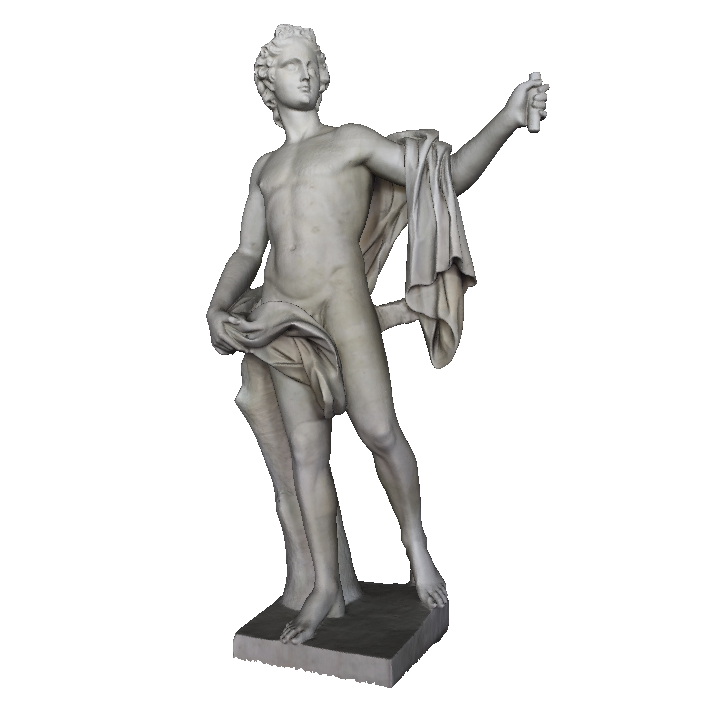
\includegraphics[width=\linewidth]{./Figures/train-dataset/00.apoll.png}
		\caption{apoll}
	\end{subfigure}
	\begin{subfigure}[b]{0.24\linewidth}
		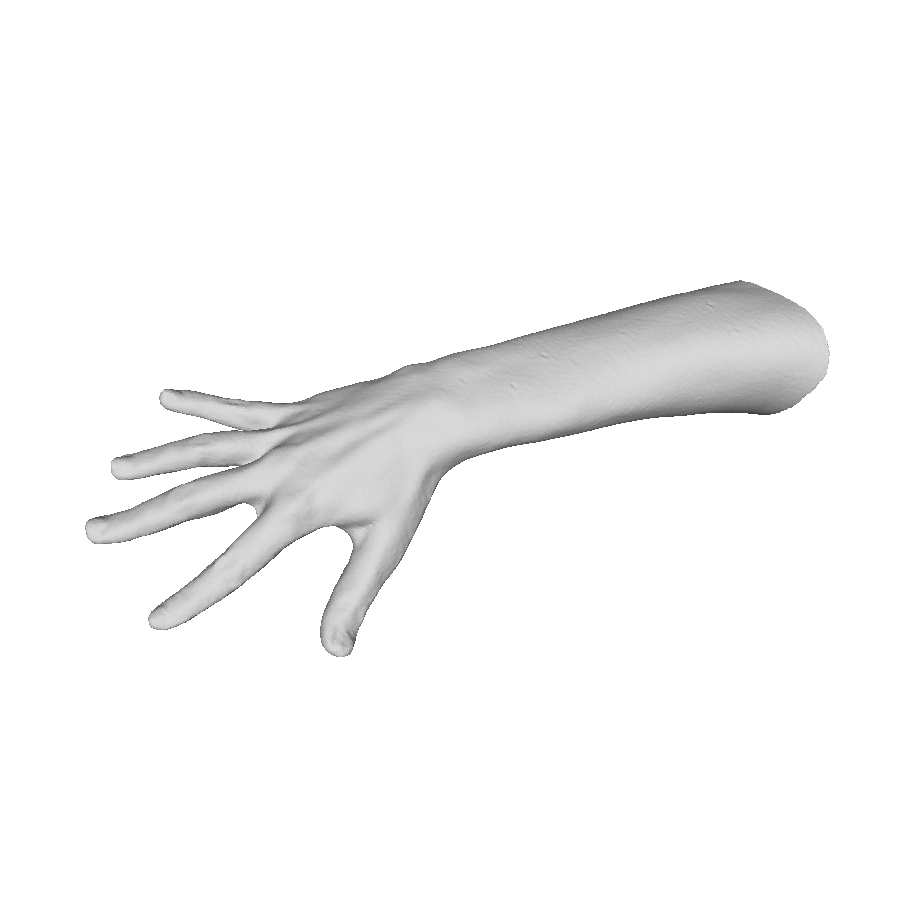
\includegraphics[width=\linewidth]{./Figures/train-dataset/01.arm.png}
		\caption{arm}
	\end{subfigure}
	\begin{subfigure}[b]{0.24\linewidth}
		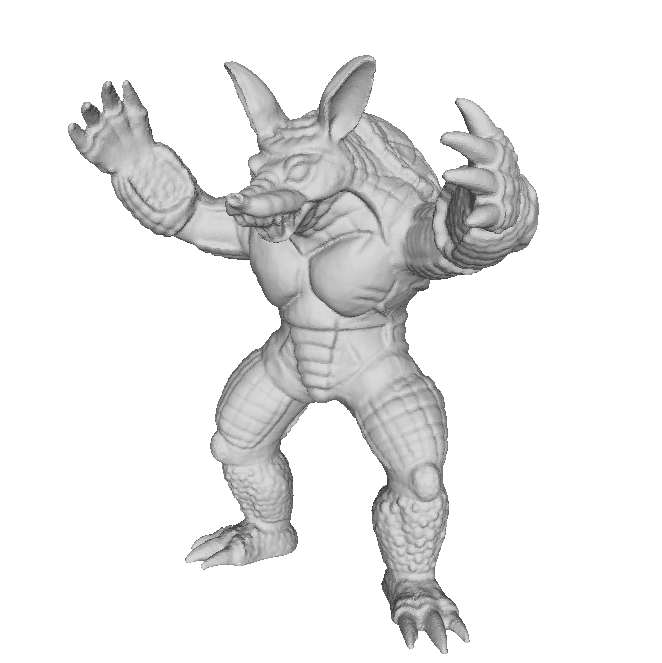
\includegraphics[width=\linewidth]{./Figures/train-dataset/02.armadillo.png}
		\caption{armadillo}
	\end{subfigure}
	\begin{subfigure}[b]{0.24\linewidth}
		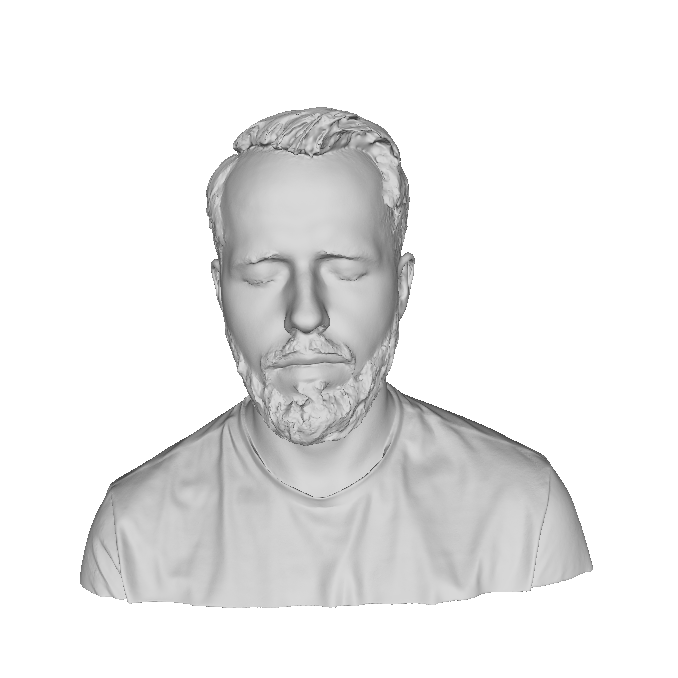
\includegraphics[width=\linewidth]{./Figures/train-dataset/03.bearded-guy.png}
		\caption{bearded-guy}
	\end{subfigure}
	
	\begin{subfigure}[b]{0.24\linewidth}
		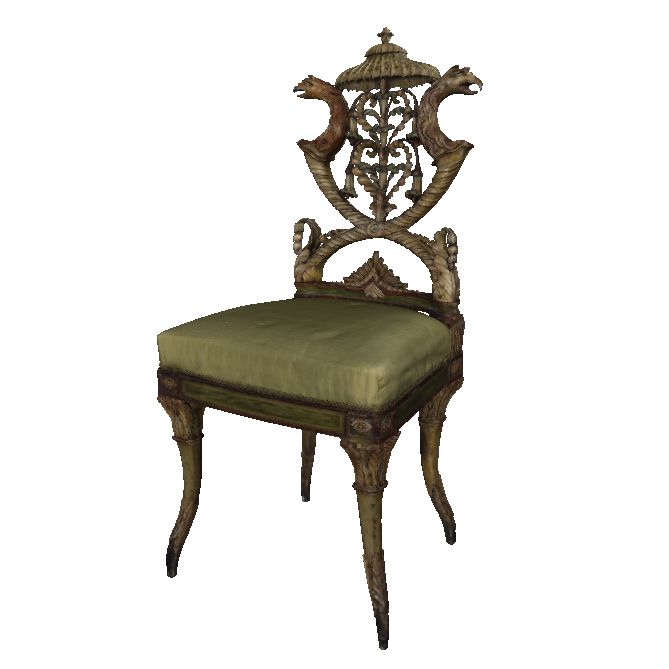
\includegraphics[width=\linewidth]{./Figures/train-dataset/08.pergolesi-side-chair_texture.png}
		\caption{chair}
	\end{subfigure}
	\begin{subfigure}[b]{0.24\linewidth}
		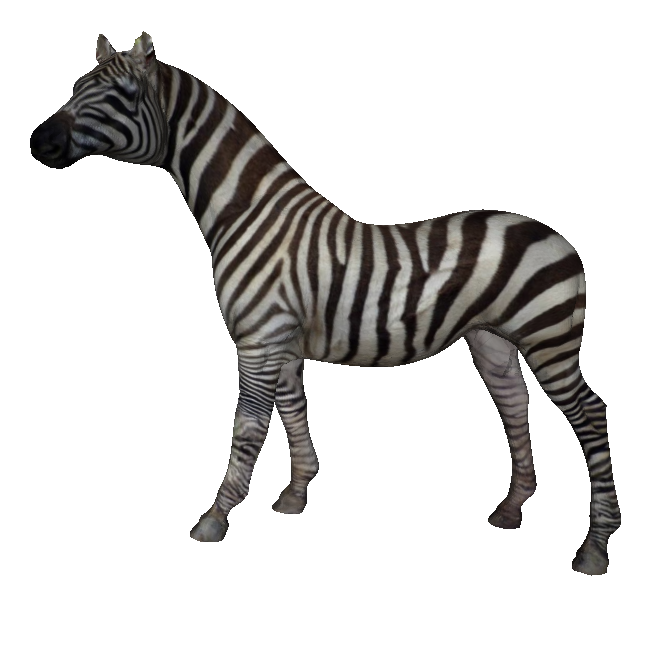
\includegraphics[width=\linewidth]{./Figures/train-dataset/42.zebra_texture.png}
		\caption{zebra}
	\end{subfigure}
	\begin{subfigure}[b]{0.24\linewidth}
		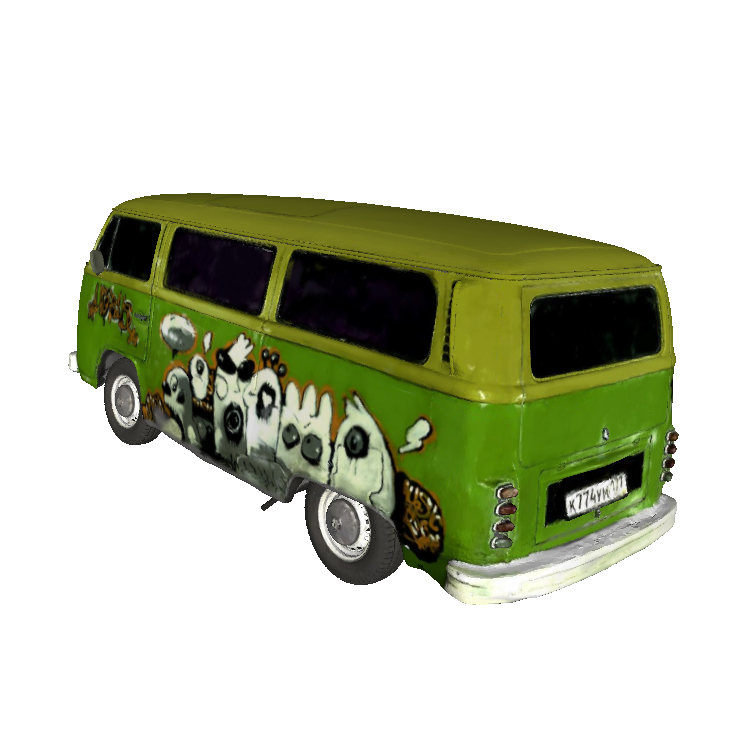
\includegraphics[width=\linewidth]{./Figures/test-dataset/01.bus_texture.png}
		\caption{bus}
	\end{subfigure}
	\begin{subfigure}[b]{0.24\linewidth}
		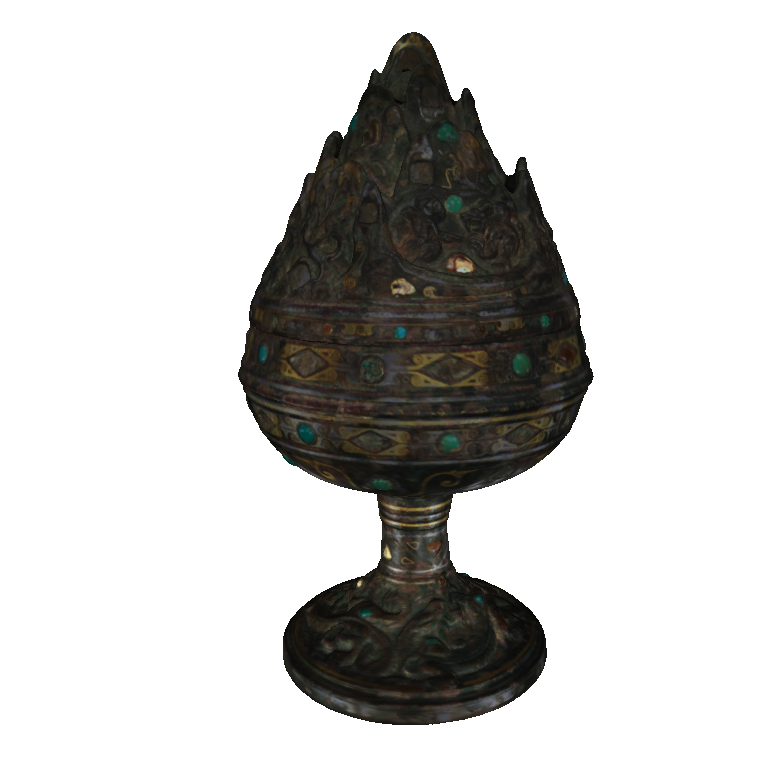
\includegraphics[width=\linewidth]{./Figures/test-dataset/03.baoshanlu_texture.png}
		\caption{baoshanlu}
	\end{subfigure}
	\decoRule
	\caption{Some of the objects used for \textit{Synthetic-50-5}}
	\label{fig:dataset-demo}
\end{figure}
In addition, some objects also have colored textures, as shown in the second line of Figure \ref{fig:dataset-demo}. This is specifically prepared for the illuminated approach, since the image is used to evaluate the surface normals. By using textured models, our models get closer to the real dataset and have improved robustness that can be further applied to the real dataset.



\definecolor{direction-light-color}{RGB}{255,244,214}
\newcommand{\col}[1]{%
	\textcolor{#1}{\vrule width 0.5cm}}
\section{Synthesizing Scenes using Unity}

To simulate the data acquisition scenario as realistically as possible. We made the following settings. A flat cylinder, called \textit{stage} , is placed in the center of the 3D space as a platform for placing objects. We fixed the \textit{stage} in a predetermined position that will not be changed when images are captured. 
A directional light with RGB color FFF4D6 \col{direction-light-color} is placed 25 m away in the top view direction as an ambient light, which also has a fixed position.
An RGB-D camera is placed about 10 m away from the stage in the top-view direction. The camera captures the depth map and the grayscale image, which are randomly arranged after each scene. The movement range of the camera is 0.1 m in both directions of the X, Y and Z axes and a randomly changed Euler angle of $ 1^\circ $. 
A point light is placed about 5 m away as the illumination light, which is also moved randomly after each scene. The range of motion is 0.3 m in both directions of the X, Y and Z axes and $ 1^\circ $ randomly in the Euler angle.

During data acquisition, the object is randomly selected and placed on the stage. The object has a random rotation of up to $ 30^\circ $ in the $roll $ axis direction, a $ 30^\circ $ rotation in the $pitch $ axis direction, and a $ 180^\circ $ degree rotation in the $yaw $ axis direction. This gives the camera the ability to capture most directions of the objects. The layout in the Unity game engine is shown in Figure \ref{fig:unity-workplace}. We generate 3000 scenes with resolution $ 128\times128 $ and 5000 scenes with resolution $ 512\times512 $.

\begin{figure}[h!]
	\centering
		\captionsetup{width=\linewidth}
	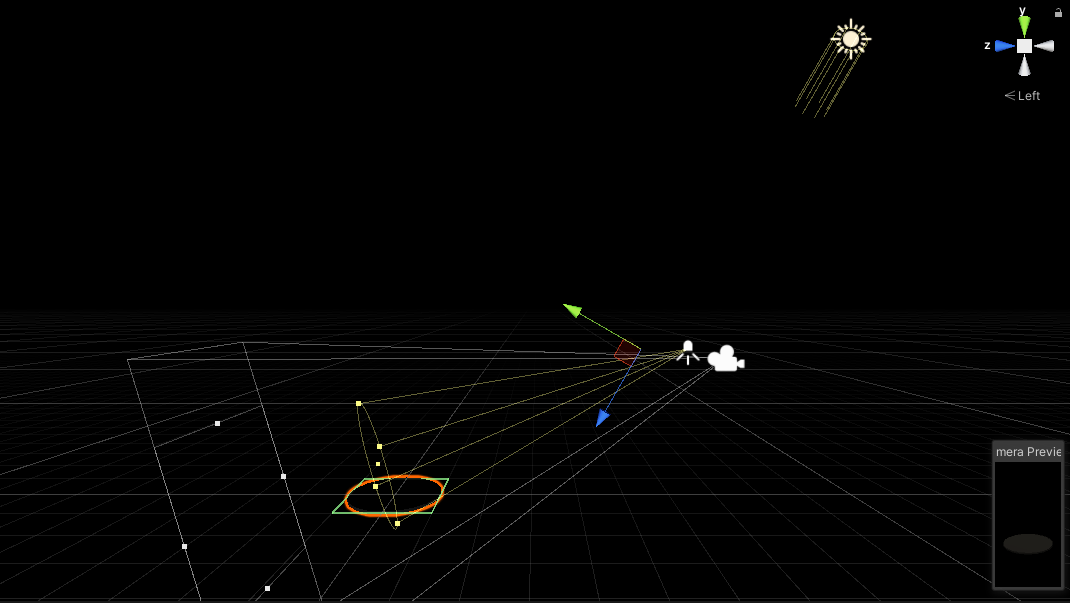
\includegraphics[width=\linewidth]{./Figures/unity-workplace.PNG}
	\decoRule
	\caption{The layout of synthetic scene generation in Unity.}
	\label{fig:unity-workplace}
\end{figure}
The main advantage of generated scenes is the availability of complete information. We can capture the depth map in a lossless way. The corresponding normal map can also be safely considered as ground truth. And the scale of the dataset is easy to control. Table \ref{tab:data-files} gives more dataset information.
\begin{table}
	\centering
	\begin{tabular}{l l}
		\toprule
		\tabhead{Data} & \tabhead{Size} \\
		\midrule
		Depth map & Width$ \times $Height$ \times $ 1 \\
		\hline 
		Depth range  & MinDepth, MaxDepth \\  
		\hline
		Grayscale Image	&  Width$ \times $Height$ \times $ 1 \\  
		\hline 
		Normal Map &   Width$ \times $Height$ \times $ 3  \\
		\hline 
		Light Position &  $ 3\times1 $  \\
		\hline
		Camera Intrinsic Matrix &  $ 3\times 3 $  \\
		\hline 
		Camera Extrinsic Matrix &  $ 3\times 4 $  \\
		\bottomrule
	\end{tabular}
	\caption{The information saved for each scene in \textit{synthetic-50-5}.}
	\label{tab:data-files}
\end{table}


A critical detail we need to pay attention to is the exposure of the camera. Or we need to control the light emission on the object surface. As can be seen in Figure \ref{fig:camera_exposure}, too much exposure causes the surface texture to be difficult to see, resulting in clipping. In our experiments, we found that an appropriate light setting is essential for the illumination-based approach. Too much or too little lighting effects do not improve the illumination-based approach.

\begin{figure}[H]
	\centering
	\captionsetup{width=\linewidth}
	\begin{subfigure}[b]{0.32\linewidth}
		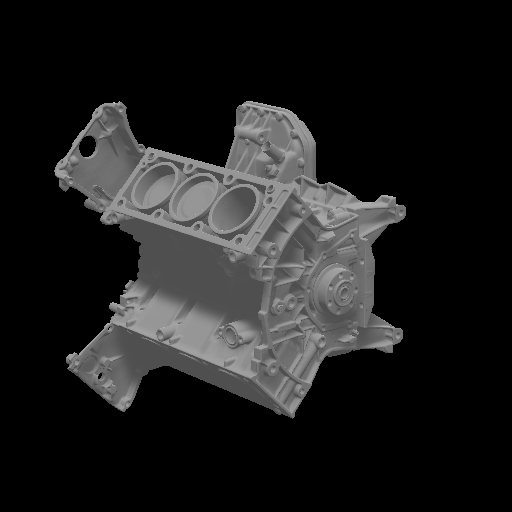
\includegraphics[width=\textwidth]{./Figures/wrong_exposure_2.png}
		\caption{Insufficient light}
	\end{subfigure}
	\begin{subfigure}[b]{0.32\linewidth}
		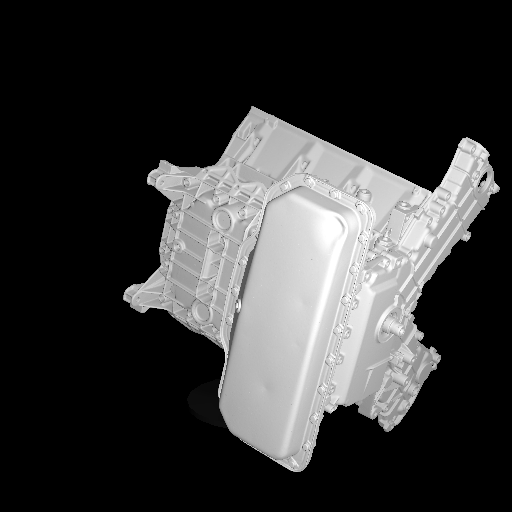
\includegraphics[width=\textwidth]{./Figures/right_exposure.png}
		\caption{Just Right}
	\end{subfigure}
	\begin{subfigure}[b]{0.32\linewidth}
		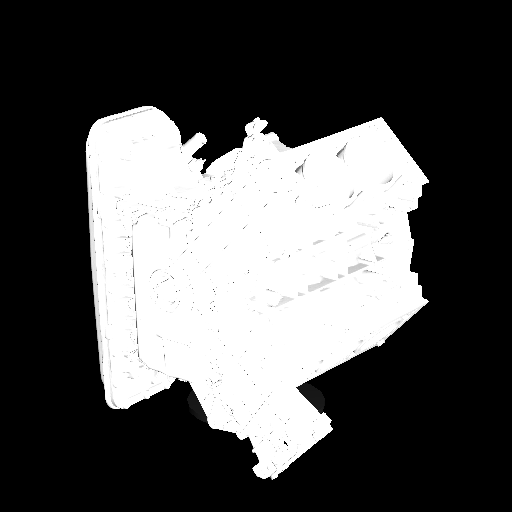
\includegraphics[width=\textwidth]{./Figures/wrong_exposure.png}
		\caption{Too much light}
	\end{subfigure}
	\decoRule
	\caption{Different exposure to the objects.}
	\label{fig:camera_exposure}
\end{figure}




\section{Data Preprocessing}
The raw data collected by Unity required further processing before it could be fed into the training models. 
\paragraph{Depth Map}
A depth map is a 1-channel image that contains information about the distance from the object surface to the camera center. It is stored as a 16-bit grayscale image, meaning that each pixel is in the range $\mathtt{0 - 65535}$. 

The raw depth maps in real data acquired by light scanners usually have missing pixels. To achieve a good match to the real data, a uniformly distributed noise was added to the synthetic data to randomly remove the valid pixels in the depth maps.
The simulated noise is uniformly distributed over the entire map with a certain noise intensity. A parameter $ \mu $ is used to control the intensity of the noise. It specifies the $ \mu $ pixel drop in percent. For example, at $ \mu-10 $, 10\% of the pixels are randomly removed. For each scene, the noise operation is based on a random $ \mu $ in a range $ \left[0, 50\right] $. In some scenes there are more missing pixels, in others less. The random noise intensity also allows the model to learn scenarios not only with noise, but also with low noise or even no noise.
Figure \ref{fig:noise-intensity} shows the noise effect at different $ \mu $.



%% add noise image
\begin{figure}[!h]
	\centering
	\captionsetup{width=\linewidth}
	{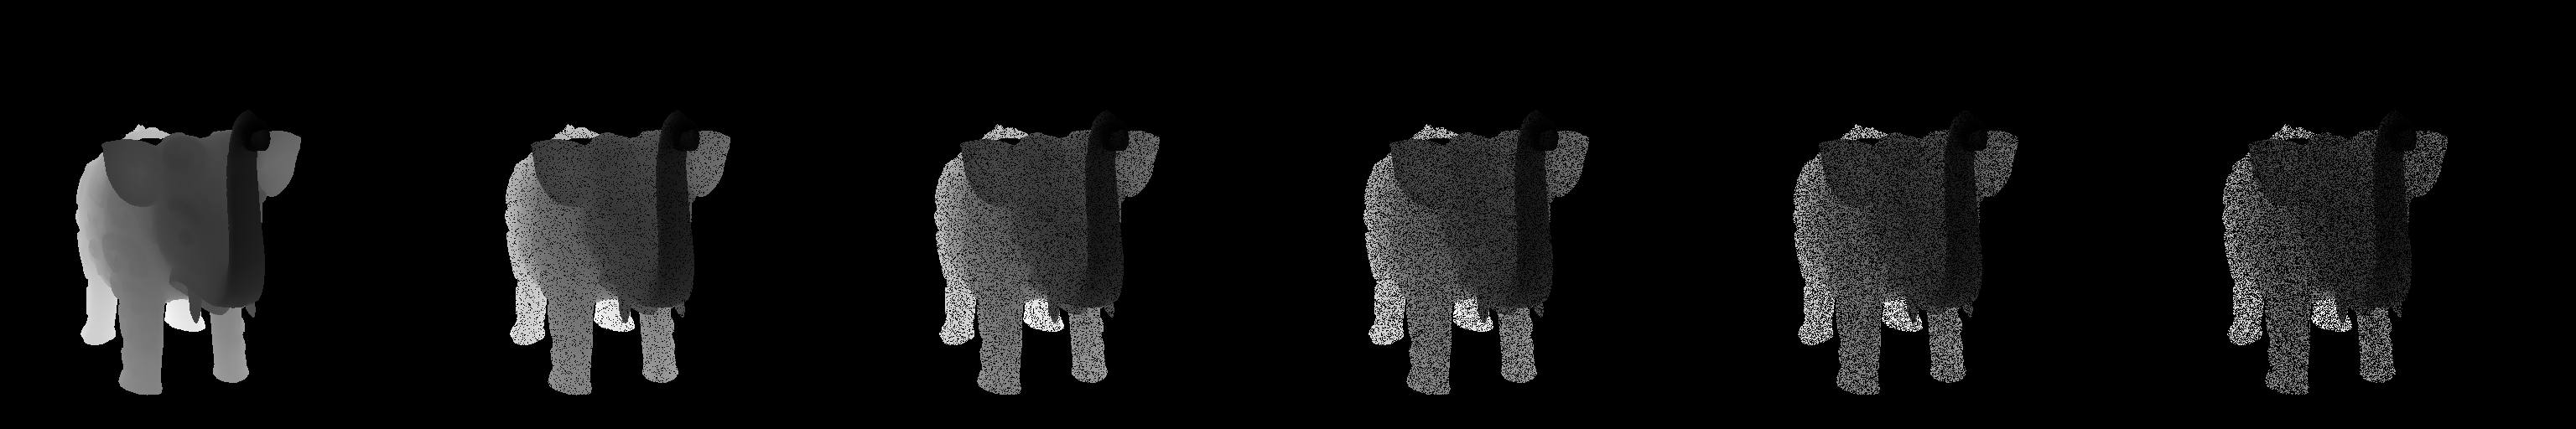
\includegraphics[width=\textwidth]{./Figures/add_noise_depth.png}}
	\decoRule
	\caption{From left to right: Noise-intensity on $ \mu-0$, $\mu-10$, $\mu-20$, $\mu-30$, $\mu-40$, $\mu-50$. Object Name: \textit{elephant-zun-lid}.}
	\label{fig:noise-intensity}
\end{figure}

%\begin{figure}[h!]
%	\centering
%	\begin{tikzpicture} 
%		% reference lines
%		\node[inner sep=10pt] (input) at (0,0)
%		{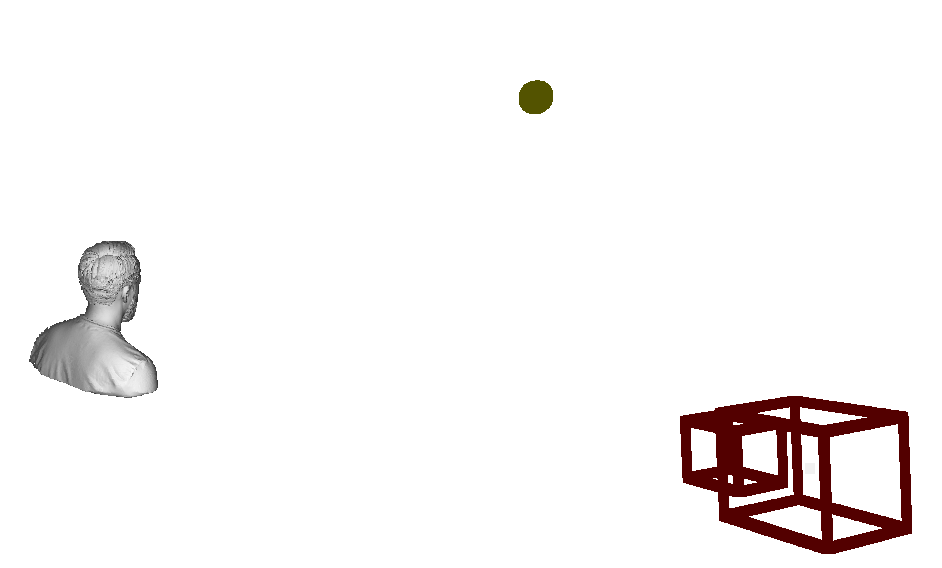
\includegraphics[width=\linewidth]{./Figures/ply_config.png}};
%		
%		%		\draw[thick,dashed]	(0,0) -- (10,0) ; % bottom
%		%		\draw[thick,dashed]	(0,3) -- (10,3) node[pos=0.9, above] {image plane}; % middle
%		%		\draw[thick,dashed]	(0,6) -- (10,6); % top
%		% camera 
%		%		\filldraw[black] (5,0) circle (2pt) node[anchor=south west]{Camera Position};
%		% world point 
%		%		\filldraw[black] (2,2) circle (2pt) node[anchor=north west]{Point};
%		% image point
%		%		\filldraw[black] (6,3) circle (2pt) node[anchor=north west]{Pixel};
%		% similiar triangles
%		%		\draw[thick] (0,0) -- (2,6); % AB
%		%		\draw[thick] (5,0) -- (7,6); % AC
%		%		\draw[thick] (5,6) -- (7,6) node[midway, below] {$ X $}; % BC
%		%		\draw[thick] (5,3) -- (6,3) node[midway, below] {$ u $};
%		%		% measure arrows
%		%		\draw[thick, <->] (4,0) -- (4,3) node[midway, left] {$ fk_u $};
%		%		\draw[thick, <->] (3,0) -- (3,6) node[pos=0.3, left] {$ Z $};
%	\end{tikzpicture}	
%	\caption{Data Collection configuration}
%	\label{fig:depth-triangulation}
%\end{figure}
The depth map is converted to a 3D vertex map after adding the noise.
Consider a 3-dimensional Euclidean space. The $ X $ and $ Y $ axes are perpendicular to each other align with the direction of width and height of the depth map separately. The $ Z $ axis is point inward (i.e., from view point to the depth map). The depth provided in the depth map is the distance from camera center to the object surface. Thus, in order to find the corresponding 3D vertex map $ \textbf{V}_C $ with respect to the camera coordinate system, we only need to multiple the depth matrix $ \textbf{Depth} $ with the point direction matrix $ \textbf{Dir} $.

\begin{dgroup*}
	\begin{dmath*}
		\textbf{V}_C = \textbf{Depth} \odot \textbf{Dir}
	\end{dmath*}
\end{dgroup*}

For the direction $ \textbf{Dir}(x,y,z) $ of a point $ \textbf{V}(x,y,z) $, it's X and Y components can be mapped from the corresponding pixel position $ (u,v) $ on the depth map, whereas the Z component is the focal length $ fk $ in pixels. Then we have to further normalize it to an unit vector.

\begin{dgroup*}
	
	\begin{dmath*}
		\textbf{Dir}(x, y, z) = \dfrac{(u, v, fk)}{\|(u, v, fk) \|_2}
	\end{dmath*}

\end{dgroup*}
Conversion of a point from the camera coordinate system to the world coordinate system using the extrinsic matrix $ R $ and $ t $
\[\textbf{V}_W = \textbf{V}_C R+t \]


%% How to represent input tensor, to make it fast converse
The sizes of the individual training objects are different. We normalized them to a unit scale so that they have a relatively similar distance from the camera.
In Figure \ref{fig:data_range} we have plotted the variations in value in each axis before normalization. Table \ref{tab:data_range} gives a quantitative evaluation of the corresponding average values. 

The normalization was performed as follows. First, the points are translated to the original point as much as possible, then the range value of an axis is chosen as the scaling factor, and the points are normalized to unit vectors. The equation is represented as follows

\begin{dgroup*}
	\begin{dmath*}
		X_n =\frac{X-\min(X)}{s}
	\end{dmath*}
	\begin{dmath*}
		Y_n = \frac{Y-\min(Y)}{s}
	\end{dmath*}
	
	\begin{dmath*}
		Z_n = \frac{Z-\min(Z)}{s}
	\end{dmath*}
	\begin{dmath*}
		s = \max(X)-\min(X)
	\end{dmath*}
\end{dgroup*}
where $ s $ is a scaling factor calculated as the range of the $ X $ axis, but theoretically it can also be the range of $ Y $ or $ Z $ axis.


\begin{figure}[!h]
	\centering
	\captionsetup{width=\linewidth}
	\begin{subfigure}[b]{0.49\linewidth}
		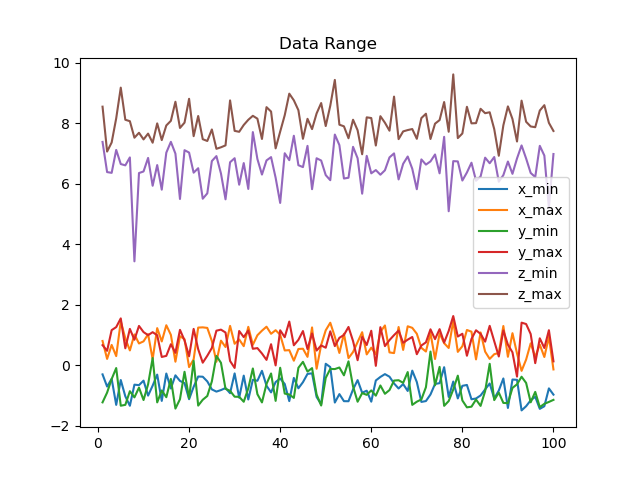
\includegraphics[width=\textwidth]{./Figures/Data_Extreme.png}
		\caption{Extreme Values in each axis }
	\end{subfigure}
	\begin{subfigure}[b]{0.49\linewidth}
		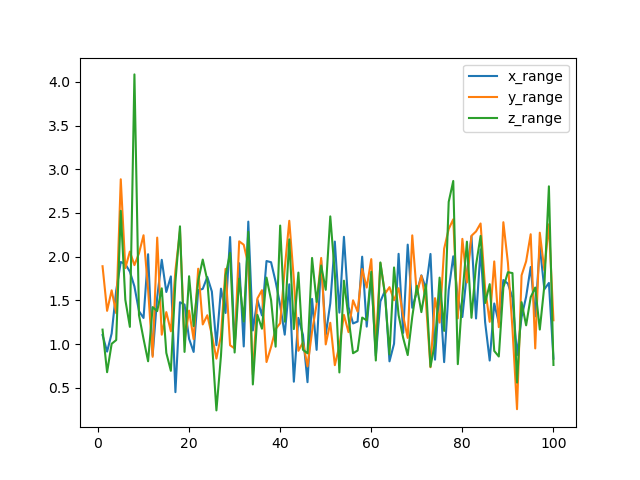
\includegraphics[width=\textwidth]{./Figures/Data_Range.png}
		\caption{Vertex Range in each axis}
	\end{subfigure}
	\decoRule
	\caption{The position fluctuation of the points in 100 Vertex Maps. 
		Left: Extreme values in 3 axes; Right: Vertex range in 3 axis.}
	\label{fig:data_range}
\end{figure}

\begin{table}[th]
	\centering
	\captionsetup{width=\linewidth}
	\begin{tabular}{c | c c c}
		\toprule
		\tabhead{Axis} & \tabhead{Scale} & \tabhead{Min} & \tabhead{Max}\\
		\midrule
		X & 1.48 & -0.75 & 0.73\\
		\hline 
		Y & 1.56 & -0.76 & 0.80\\
		\hline 
		Z & 1.47 & 6.53 & 8.00\\
		\bottomrule
	\end{tabular}
	\caption{ The fluctuation of extreme values and their ranges in 100 random training items. }
	\label{tab:data_range}
\end{table}




\paragraph{Image}

The grayscale image can be used for the photometric stereo method and also as readable information for humans. Since the image captured by the camera is in RGB format, we need to convert it to grayscale to fit our models. This is done using the following equation.
\[ gray: \frac{R+2G+B}{4}  \]

\paragraph{Normal Map}
The normal map is the tangential surface normal stored in an 8-bit/channel RGB image. The surface normal $ (n_x, n_y, n_z) $ and the corresponding RGB color $ (R,G,B) $ can be converted using the following equation:

\begin{dgroup*}
	\begin{dmath*}
		n_x = \frac{R}{255} \cdot 2 - 1
	\end{dmath*}
	\begin{dmath*}
		n_y = \frac{G}{255} \cdot 2 - 1
	\end{dmath*} 
	\begin{dmath*}
		n_z = 1-\frac{B}{255} \cdot 2
	\end{dmath*}
\end{dgroup*}

%In order to save training time, we compress the dataset in PyTorch format. The structure of a single item is shown in Table \ref{tab:tensor-structure}.
%\begin{table}[H]
%	\centering
%	\captionsetup{width=\linewidth}
%	\begin{tabular}{l | l}
%		\toprule
%		\tabhead{Name} & \tabhead{Content} \\
%		\midrule
%		\multirow{3}{*}{input-tensor}  & Vertex \\  & Image \\  & Light Direction \\
%		\hline
%		\multirow{3}{*}{output-tensor}  & GT-Normal \\ & Image \\ & GT-Light-Direction \\
%		\hline
%		Light position & light position \\
%		\hline 
%		Camera Matrix  & K,R,t\\
%		\hline 
%		Depth Range  & minDepth, maxDepth\\
%		\bottomrule
%	\end{tabular}
%	\caption{The structure of a single tensor in the dataset.}
%	\label{tab:tensor-structure}
%\end{table}
 

\chapter{Experiments} % Main chapter title

\section{Training Details}

The models are trained on the dataset \textit{synthetic-50-5} with 3000 scenes mentioned in chapter \ref{ch:04}. Each scene has a depth map with dimension $ 128\times 128 $ in height and width, an image with dimension $ 128\times 128 $. The depth map is converted from the 3D vertex map as introduced in chapter \ref{ch:04}. The light map is computed from the vertex map and the known light position. We create a tensor in PyTorch containing the vertex map, image, and light direction for each scene and consider it as a training case. Thus, 3000 scenes correspond to 3000 training cases. For each scene, there is a corresponding ground truth normal map for loss calculation and evaluation. Figure \ref{fig:test-scene} shows some of the training cases. Note that the position of the objects is not always placed naturally on the stage, but with a random rotation in the X, Y and Z axes.

% test scene
\begin{figure}[H]
	\centering
	\captionsetup{width=\linewidth}
	\begin{subfigure}[b]{0.24\linewidth}
		
\includegraphics[width=\linewidth]{./Figures/test_scenes/03094.depth0.png}
	\end{subfigure}
	\begin{subfigure}[b]{0.24\linewidth}
		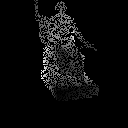
\includegraphics[width=\linewidth]{./Figures/test_scenes/03094.depth0_noise.png}
	\end{subfigure}
	\begin{subfigure}[b]{0.24\linewidth}
		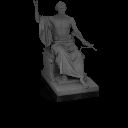
\includegraphics[width=\linewidth]{./Figures/test_scenes/03094.image0.png}
	\end{subfigure}
	\begin{subfigure}[b]{0.24\linewidth}
		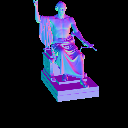
\includegraphics[width=\linewidth]{./Figures/test_scenes/03094.normal0.png}
	\end{subfigure}
	
	
	\begin{subfigure}[b]{0.24\linewidth}
		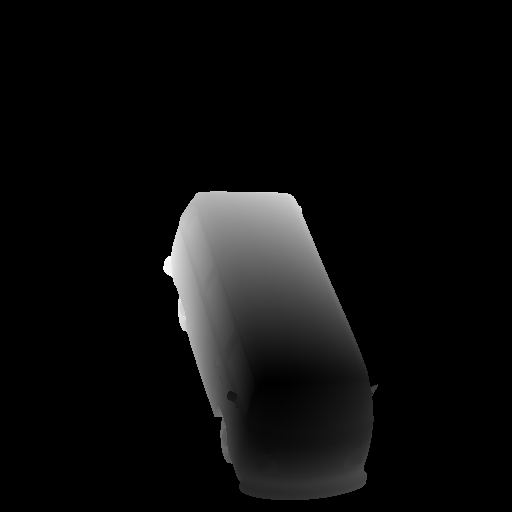
\includegraphics[width=\linewidth]{./Figures/test_scenes/05126.depth0.png}
		\caption{Depth Map}
	\end{subfigure}
	\begin{subfigure}[b]{0.24\linewidth}
		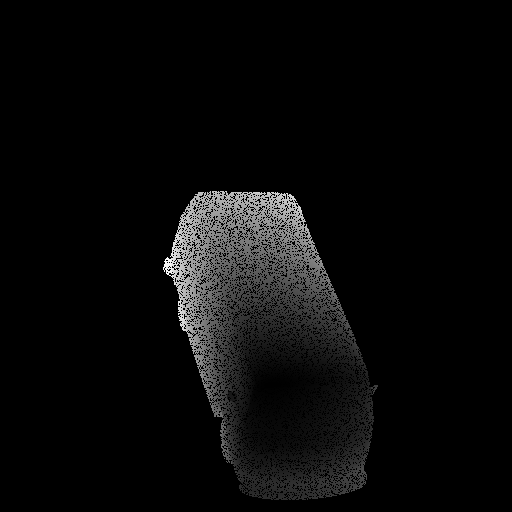
\includegraphics[width=\linewidth]{./Figures/test_scenes/05126.depth0_noise.png}
		\caption{Added noise}
	\end{subfigure}
	\begin{subfigure}[b]{0.24\linewidth}
		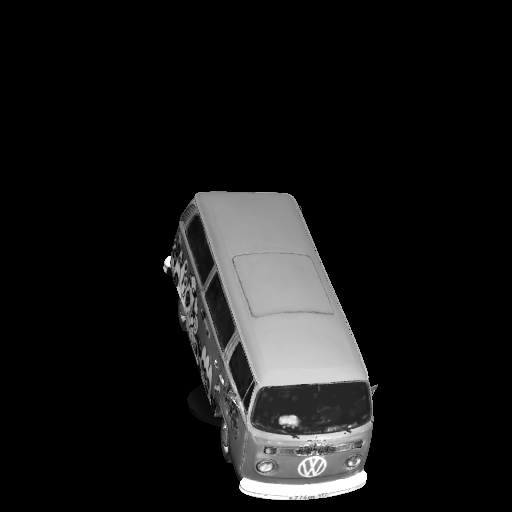
\includegraphics[width=\linewidth]{./Figures/test_scenes/05126.image0.png}
		\caption{Image}
	\end{subfigure}
	\begin{subfigure}[b]{0.24\linewidth}
		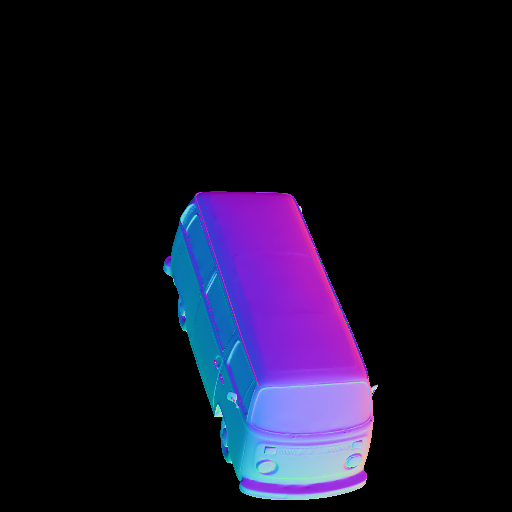
\includegraphics[width=\linewidth]{./Figures/test_scenes/05126.normal0.png}
		\caption{Normal Map}
	\end{subfigure}
	\decoRule
	\caption{Some of the evaluation scenes during the training. The objects from top to bottom rows: \textit{ Washington}, \textit{Bus}}
	\label{fig:test-scene}
\end{figure}


Besides the 3000 training scenes, 100 additional scenes with 5 different object models are used as evaluation dataset during the training. They are evaluated in each epoch. 

For the training parameters, we set the training pipeline with a batch size of 8, since we found that a higher batch size decreases the final performance.  Adam Optimizer (\cite{adam}), learning rate starting at $ 1\times10^{-3} $, it will decrease at epoch 8 with learning decay factor 0.5. The model is trained using PyTorch 1.10.0a0, CUDA 11.4.1, GPU with an NVIDIA GEFORCE RTXA 6000. It takes 14 hours to train the GCNN and 35 hours to train the Trip-Net. We stop training when the angular error of the normal map stops decreasing.


The \textit{GCNN} is the base model of the whole work. The architecture is described in \ref{sec:gcnn}. We use a single \textit{GCNN} to estimate surface normals as a geometry-based approach. It uses a vertex map as input. To verify the applicability of the skip-connection and gated-convolution layers, we trained two additional models for comparison. 
In the first model, we replace all gated layers with default convolutional layers in the network, but keep all other settings and give it the name \textit{CNN}. It is used to compare the performance between the gated layer and the default convolutional layer for our normal inference task. As mentioned in \ref{ch:03}, the gated layer is designed to process noisy input. Since the entire vertex map in the dataset was noisy, the \textit{GCNN} should outperform \textit{CNN}. 
Another model called \textit{NOC} is used to check skip connections, which simply removes the skip connections in the network but leaves the other settings unchanged. Its purpose is to show to what extent the performance of the model is improved by skipping connections. We use Reversed Huber Loss as a loss function during training. We have found that it gives a better final error compared to L2 loss. 



\begin{table}[H]
	\centering
	\captionsetup{width=\linewidth}
	\begin{tabular}{l | l l l l l }
		\toprule
		\tabhead{Model} & $ \# $\textbf{Total} &\textbf{ V-P} & \textbf{L-P} & \textbf{I-P} & \tabhead{Size /MB}\\
		\midrule
		\hline
		CNN 					& 17 & 32 & - & - & 25.5 \\
		\hline
		NOC 					& 32 & 32 & - & - & 30.6 \\
		\hline
		GCNN 					& 32 & 32 & - & - & 45.8 \\
		\bottomrule
	\end{tabular}
	\caption{GCNN model information. The V-P, L-P, and I-P columns indicate the number of convolutional layers in the vertex pipe, light pipe, and image pipe, respectively. Note that a gated convolution layer consists of 2 standard layers and is therefore counted as 2.}	
	\label{tab:gcnn-eval-mean}
\end{table}


The trip-net model uses a triple GCNN architecture with 4 fusions, which is more difficult to train. It takes the calibrated illuminated RGB-D images as input to estimate the surface normal map. When we train this model, we take the GCNN model as the baseline to observe the advantages of the illuminated information with the trip-net architecture.
We also examined the optimal fusion times of the Trip-Net to determine a possible simplification of the model. A set of similar models was trained with the same settings but different fusion times, denoted Trip-Net-F$ x $, where $ x $ denotes the fusion times. We score the fusion times from 1 to 4. For the learning rate, we initially set $ 1e-3 $. This fits the GCNN model well, but leads to a loss explosion in the trip-net. Therefore, we set a learning rate schedule with an additional decay step at epoch 8. The decay factor is $ 0.5$. The batch size is set to 8.

During training, we found that the trip-net with 4 fusions converges significantly faster than models with fewer fusion times. However, model F3 with three times fusion converges slower than F4, but ends up with a similar loss of score as F4 (see Qualitative Evaluation). Models F1 and F2 are relatively less accurate than the other two models, but the sacrifice of accuracy results in a relatively lighter model. Since they have fewer fusion times, the corresponding upsampling layers in the image and light pipes can also be removed. The model can be trained faster, and the size is also smaller. Table \ref{tab:trip-net-size-compare} contains a comparison of the size of different models.



\begin{table}[H]
	\centering
	\captionsetup{width=\linewidth}
	\begin{tabular}{l | l l l l l }
		\toprule
		\tabhead{Model} & $ \# $\textbf{Total} &\textbf{ V-P} & \textbf{L-P} & \textbf{I-P} & \tabhead{Size /MB}\\
		\midrule
		Trip-Net-F1F  			& 88 &  40 & 24 & 24 & 106\\ 
		\hline
		Trip-Net-F2F 			& 92 & 40 & 26 & 26 & 137 \\ 
		\hline
		Trip-Net-F3F 			& 96 & 40 & 28 & 28 & 167 \\
		\hline
		Trip-Net 				& 100 & 40 & 30 & 30 & 198\\
		\bottomrule
	\end{tabular}
	\caption{Trip-Net Model information. Columns V-P, L-P and I-P represent the number of convolution layers in vertex pipe, light pipe and image pipe respectively. Note that one gated convolution layer is constructed with 2 standard layers, thus it is counted as 2. }	
	\label{tab:trip-net-size-compare}
\end{table}


\section{Quantitative Evaluation on 6 Metrics}
We evaluated our models on a synthetic dataset with a resolution of $ 128 by $ 128. 
Based on the metrics proposed by \cite{geometry_based_solution}, 6 different metrics are used for the evaluation. Note that the vertex map input is only semi-dense. One of the advantages of the GCNN architecture is that it is robust to noisy input, so all points, including missing points in the input vertex map, are considered in the evaluation. We use $\tilde{\textbf{N}}$ for the estimated normal map, $ \textbf{N} $ for the ground-truth normal map, $ P $ for the \textit{set} of valid points, \textit{ValidNum} for the number of valid points. \textit{abs} is a function to calculate the absolute value of the given values, \textit{median} is a function to calculate the median value of a given \textit{set}.



\paragraph{Average Angle Error Metric (AAE)}
The metric calculates the average absolute angular error for each point between the inferred normal and the ground-truth normal map.
%% https://www.cuemath.com/geometry/angle-between-vectors/
\[ 
AAE = \frac
{1}
{ValidNum} \cdot \sum_{i\in P}  \left|   \arccos \frac{\textbf{N}_{i}\cdot \tilde{\textbf{N}}_{i}} {| \textbf{N}_{i} |  |\tilde{\textbf{N}}_{i}|  } \cdot  \frac{180}{\pi}   \right| 
\]

\paragraph{Median Angle Error Metric (MED)}
The metric calculates the median of the absolute angular error of all points in the normal map.

\[ 
MED = 
\text{Median}   \left( \Bigg\{ \left|\arccos \frac{\textbf{N}_{i}\cdot \tilde{\textbf{N}}_{i}} {| \textbf{N}_{i} |  |\tilde{\textbf{N}}_{i}|  } \right| \text{for}\ i \in P   \Bigg\}\right)
\]

\paragraph{5 Degree Error Metric ($ E_5 $)}
The metric calculates the percentage of predicted normals that have an error less than $ 5^\circ $ compared to ground truth. First, the number of normals that have an error less than $ 5^\circ $ ($ D_5 $) is calculated.
\[
D_5 = \sum_{i\in P} \left( \text{abs}\left(   \arccos \frac{\textbf{N}_{i}\cdot \tilde{\textbf{N}}_{i}} {| \textbf{N}_{i} |  |\tilde{\textbf{N}}_{i}|  } \cdot  \frac{180}{\pi}   \right) < 5 \right)
\]
Then the percentage of normals that have error less than $ 5^\circ $ ($ E_5 $) is calculated.
\[ 
E_5 = \frac{D_5}{ValidNum}\times 100\%
\]


\paragraph{11.5 Degree Error Metric ($ E_{11.5} $)}
The metric calculates the percentage of predicted normals that have an error less than $ 11.5^\circ $ compared to ground truth. First, the number of normals that have an error less than $ 11.5^\circ $ ($ D_{11.5} $) is calculated.

\[
D_{11.5} = \sum_{i\in P} \left( \text{abs}\left(   \arccos \frac{\textbf{N}_{i}\cdot \tilde{\textbf{N}}_{i}} {| \textbf{N}_{i} |  |\tilde{\textbf{N}}_{i}|  } \cdot  \frac{180}{\pi}   \right) < 11.5 \right)
\]
Then the percentage of normals that have error less than $ 11.5^\circ $ ($ E_{11.5} $) is calculated.
\[ 
E_{11.5} = \frac{D_{11.5}}{ValidNum}\times 100\%
\]

\paragraph{22.5 Degree Error Metric ($ E_{22.5} $)}
The metric calculates the percentage of predicted normals that have an error less than $ 22.5^\circ $ compared to ground truth. First, the number of normals that have an error less than $ 22.5^\circ $ ($ D_{22.5} $) is calculated.

\[
D_{22.5} = \sum_{i\in P} \left( \text{abs}\left(   \arccos \frac{\textbf{N}_{i}\cdot \tilde{\textbf{N}}_{i}} {| \textbf{N}_{i} |  |\tilde{\textbf{N}}_{i}|  } \cdot  \frac{180}{\pi}   \right) < 22.5 \right)
\]
Then the percentage of normals that have error less than $ 22.5^\circ $ ($ E_{22.5} $) is calculated.
\[ 
E_{22.5} = \frac{D_{22.5}}{ValidNum}\times 100\%
\]


\paragraph{30 Degree Error Metric ($ E_{30} $)} 
The metric calculates the percentage of predicted normals that have an error less than $ 30^\circ $ compared to ground truth. First, the number of normals that have an error less than $ 30^\circ $ ($ D_{30} $) is calculated.

\[
D_{30} = \sum_{i\in P} \left( \text{abs}\left(   \arccos \frac{\textbf{N}_{i}\cdot \tilde{\textbf{N}}_{i}} {| \textbf{N}_{i} |  |\tilde{\textbf{N}}_{i}|  } \cdot  \frac{180}{\pi}   \right) < 30 \right)
\]
Then the percentage of normals that have error less than $ 30^\circ $ ($ E_{30} $) is calculated.
\[ 
E_{30} = \frac{D_{30}}{ValidNum}\times 100\%
\]

We evaluated our trained models on \textit{synthetic-50-5}. In the test dataset, 5 objects are considered. They are: \textit{Baoshanlu}, \textit{Bus}, \textit{Dragon}, \textit{Garfield} and \textit{Washington}. Each object has 20 scenes with a total of 100 scenes for 5 objects. The test objects are not present in the training dataset. We evaluate all the presented models on the test dataset, to fit them into a table, the names of each model are simplified. The model \textit{SVD} uses the SVD optimization method, the model \textit{NOC} is the no-skip connection version of \textit{GCNN}, \textit{CNN} is the CNN version of \textit{GCNN}. \textit{F1}, \textit{F2}, \textit{F3}, \textit{F4} are the fusion times in the \textit{Trip-Net}. 




When evaluating the \textit{GCNN} models, we take \textit{SVD} model with an optimal neighborhood size as baseline. \textit{NOC} and \textit{CNN} are used to verify the performance of \textit{GCNN} model. When evaluate the \textit{F1}-\textit{F4} models, we can take \textit{GCNN} model as baseline. 

From the table we can see that all the learning based approaches achieves a better result than SVD approach. In the 30 degrees error metric, GCNN based approach achieves 95 \% accuracy whereas Trip-Net is even higher, some of the models like \textit{dragon} achieves 98\%. The best performance is around 90\%, 75 \%, 45 \% in $ 22.5^\circ $, $ 11.5^\circ $ and $ 5^\circ $ degrees error metrics respectively. Another notable result is the close performance of F3 and F4 models, where they achieves a very comparable performance. We also found that during the training, F4 model converges faster than F3, but F3 in the end achieves a similar loss with model F4. However, based on the $ 30^\circ $, $ 22.5^\circ $, $ 11.5^\circ $ metrics, we can still see that F4 model gives a more stable performance with less high error normals. This is reasonable since the last fusion in the original resolution provides more high resolution information to the models.



In evaluating the \textit{GCNN} models, we take the \textit{SVD} model with an optimal neighborhood size as the baseline. \textit{NOC} and \textit{CNN} are used to check the performance of the \textit{GCNN} model. When evaluating the \textit{F1}-\textit{F4} models, we can take the \textit{GCNN} model as a baseline. 

From the table, it can be seen that all learning-based approaches achieve a better result than the \textit{SVD} approach. In the 30-degree error metric, the GCNN-based approach achieves 95\% accuracy, while Trip-Net is even higher and some models such as \textit{dragon} achieve 98\%. 
The best performance is 90\%, 75\%, 45\% in the $ 22.5^\circ $, $ 11.5^\circ $ and $ 5^\circ $ degree error metric, respectively. Another notable result is the close relationship between the F3 and F4 models, which achieve very comparable performance. We also found that model F4 converges faster than F3 during training, but F3 ends up achieving a similar loss as model F4. However, using the metrics $ 30^\circ $, $ 22.5^\circ $ and $ 11.5^\circ $, we can see that the F4 model has a more stable performance with less high error normals. This is reasonable since the last fusion at the original resolution provides more high-resolution information to the models.


%% mean metric
\begin{table}[H]
	\centering
	\captionsetup{width=\linewidth}
	\begin{tabular}{l | l | l l l | l l l l }
		\toprule
		\tabhead{Object} & \tabhead{SVD} & \tabhead{GCNN} & \tabhead{NOC} & \tabhead{CNN} & \tabhead{F1}& \tabhead{F2}& \tabhead{F3}& \tabhead{F4}\\
		\midrule
		Baoshanlu  		& 35.66 & 11.09 & 13.58 & 15.55 & 11.22 & 10.36 &\textbf{ 9.77 }& 9.80 \\ 
		\hline
		Bus 			& 31.93 & 7.79 & 8.95 & 11.93 & 7.49 & 7.85 & \textbf{7.30} & 7.62\\ 
		\hline
		Dragon 			& 39.57 & 10.60 & 15.29 & 16.03 & 10.47 & 10.23 & 8.16 &\textbf{ 7.79} \\
		\hline
		Garfield 		& 39.69 & 10.20 & 12.50 & 14.46 & 9.94 & 10.36 & 9.71 &\textbf{ 9.39} \\
		\hline
		Washington 		& 42.83 & 13.43 & 17.59 & 18.71 & 13.32 & 13.40 & 12.62 &\textbf{ 12.60}\\
		\bottomrule
	\end{tabular}
	\caption{Average angular error of the evaluation dataset. \textit{SVD} Neighborhood size $ k=2 $}	
	\label{tab:eval-mean}
\end{table}

%% median metric
\begin{table}[H]
	\centering
	\captionsetup{width=\linewidth}
	\begin{tabular}{l | l | l l l | l l l l }
		\toprule
		\tabhead{Object} & \tabhead{SVD} & \tabhead{GCNN} & \tabhead{NOC} & \tabhead{CNN} & \tabhead{F1}& \tabhead{F2}& \tabhead{F3}& \tabhead{F4}\\
		\midrule
		Baoshanlu  		& 34.06 & 8.86 & 10.82 & 13.25 & 8.95 & 8.02 & 7.54 &\textbf{ 7.50} \\ 
		\hline
		Bus 			& 34.14 & 4.44 & 5.02 & 8.69 & 4.11 & 4.58 & \textbf{3.65 }& 4.47 \\ 
		\hline
		Dragon 			& 36.43 & 7.62 & 11.10 & 13.26 & 7.60 & 7.12 & 5.87 &\textbf{ 5.52} \\
		\hline
		Garfield 		& 37.60 & 6.40 & 8.90 &11.31 & 6.30 & 6.72 & 6.21 & \textbf{6.04 }\\
		\hline
		Washington 		& 36.89 & 7.64 & 11.38 & 13.64& 7.49 & 7.60 &\textbf{ 7.03 }& 7.25\\
		\bottomrule
	\end{tabular}
	\caption{Median angular error of the evaluation dataset. \textit{SVD} Neighborhood size $ k=2 $}	
	\label{tab:eval-median}
\end{table}


%% 5 degree metric
\begin{table}[H]
	\centering
	\captionsetup{width=\linewidth}
	\begin{tabular}{l | l | l l l |l l l l }
		\toprule
		\tabhead{Object} & \tabhead{SVD} & \tabhead{GCNN} & \tabhead{NOC} & \tabhead{CNN} & \tabhead{F1}& \tabhead{F2}& \tabhead{F3}& \tabhead{F4}\\
		\midrule
		Baoshanlu  		& 0.01 & 0.25 & 0.18 & 0.11 & 0.24 & 0.31 &\textbf{ 0.33 }& 0.32\\ 
		\hline
		Bus 			& 0.00 & 0.56 & 0.50 & 0.23 & 0.59 & 0.54 & \textbf{0.63 }& 0.55 \\ 
		\hline
		Dragon 			& 0.00 & 0.31 & 0.17 & 0.10 & 0.31 & 0.34 & 0.43 &\textbf{ 0.46}\\
		\hline
		Garfield 		& 0.00 & 0.41 & 0.27 & 0.14 & 0.42 & 0.39 & 0.42 & \textbf{0.43}\\
		\hline
		Washington 		& 0.00 & 0.38 & 0.26 & 0.10 & 0.36 & 0.36 & \textbf{0.40 }& 0.37\\
		\bottomrule
	\end{tabular}
	\caption{Percentage of error of less than 5 degrees of the evaluation data set. \textit{SVD} Neighborhood size $ k=2 $}	
	\label{tab:eval-5d}
\end{table}


%% 11.5 degree metric
\begin{table}[H]
	\centering
	\captionsetup{width=\linewidth}
	\begin{tabular}{l | l | l l l | l l l l }
		\toprule
		\tabhead{Object}  & \tabhead{SVD} & \tabhead{GCNN} & \tabhead{NOC} & \tabhead{CNN} & \tabhead{F1}& \tabhead{F2}& \tabhead{F3}& \tabhead{F4}\\
		\midrule
		Baoshanlu  		& 0.03 & 0.62 & 0.52 & 0.41 &  0.62 & 0.66 &\textbf{ 0.69 }& \textbf{0.69}\\ 
		\hline
		Bus 			& 0.05 & 0.81 & 0.78 & 0.65 & 0.83 & 0.82 & \textbf{0.83 }&\textbf{ 0.83 }\\ 
		\hline
		Dragon 			& 0.02 & 0.69 & 0.51 & 0.40 & 0.70 & 0.71 & 0.79 & \textbf{0.81}\\
		\hline
		Garfield 		& 0.03 & 0.72 & 0.62 & 0.51 &0.73 & 0.71  & 0.74 &\textbf{ 0.75}\\
		\hline
		Washington 		& 0.02 & 0.62 & 0.50 & 0.40 & 0.63 & 0.62 & 0.64 & \textbf{0.65}\\
		\bottomrule
	\end{tabular}
	\caption{Percentage of error of less than 11.5 degrees of the evaluation data set. \textit{SVD} Neighborhood size $ k=2 $}	
	\label{tab:eval-11d}
\end{table}



%% 22.5 degree metric
\begin{table}[H]
	\centering
	\captionsetup{width=\linewidth}
	\begin{tabular}{l | l | l l l | l l l l }
		\toprule
		\tabhead{Object}  & \tabhead{SVD} & \tabhead{GCNN} & \tabhead{NOC} & \tabhead{CNN} & \tabhead{F1}& \tabhead{F2}& \tabhead{F3}& \tabhead{F4}\\
		\midrule
		Baoshanlu  		& 0.18 & 0.90 & 0.84 & 0.79 & 0.90 & 0.91 &\textbf{ 0.92} &\textbf{ 0.92}\\ 
		\hline
		Bus 			& 0.26 & 0.93 & 0.91 & 0.89 & 0.93 & 0.93 & 0.93 & \textbf{0.94}\\ 
		\hline
		Dragon 			& 0.14 & 0.90 & 0.79 & 0.80 & 0.90 & 0.90 & 0.94 & \textbf{0.95}\\
		\hline
		Garfield 		& 0.13 & 0.89 & 0.86 & 0.84 & 0.90 & 0.89 &\textbf{ 0.91} &\textbf{ 0.91}\\
		\hline
		Washington 		& 0.14 & 0.81 & 0.72 & 0.72 & 0.81 & 0.81 & \textbf{0.83} &\textbf{ 0.83}\\
		\bottomrule
	\end{tabular}
	\caption{Percentage of error of less than 22.5 degrees of the evaluation data set. \textit{SVD} Neighborhood size $ k=2 $}	
	\label{tab:eval-22d}
\end{table}


%% 30 degree metric
\begin{table}[H]
	\centering
	\captionsetup{width=\linewidth}
	\begin{tabular}{l | l | l l l | l l l l }
		\toprule
		\tabhead{Object} & \tabhead{SVD} & \tabhead{GCNN} & \tabhead{NOC} & \tabhead{CNN} & \tabhead{F1}& \tabhead{F2}& \tabhead{F3}& \tabhead{F4}\\
		\midrule
		Baoshanlu  		& 0.37 & 0.96 & 0.93 & 0.90 & 0.96 & 0.96 &\textbf{ 0.97 }&\textbf{ 0.97} \\ 
		\hline
		Bus 			& 0.43 & 0.96 & 0.94 & 0.93 & 0.96 & \textbf{0.96} &\textbf{ 0.96} &\textbf{ 0.96 }\\ 
		\hline
		Dragon 			& 0.30 & 0.95 & 0.88 & 0.90 & 0.95 & 0.95 & 0.97 & \textbf{0.98} \\
		\hline
		Garfield 		& 0.27 & 0.94 & 0.92 & 0.91 & 0.94 & 0.94 & 0.94 & \textbf{0.95 }\\
		\hline
		Washington 		& 0.28 & 0.88 & 0.81 & 0.82 & 0.88 & 0.88 & \textbf{0.89} & \textbf{0.89}\\
		\bottomrule
	\end{tabular}
	\caption{Percentage of error of less than 30 degrees of the evaluation data set. \textit{SVD} Neighborhood size $ k=2 $}	
	\label{tab:eval-30d}
\end{table}



%% svd evaluation
\section{Visual Evaluation on SVD}

The \textit{SVD} approach can predict the normal map well if the given point cloud is dense. As shown in figure \ref{fig:svd-normal}. It can successfully predict the smooth surface of the dragon object, especially the flakes and the tails of the dragon. 

However, it fails in the areas such as the hind leg, horn, and mouth, which are mainly composed of sharp edges. This is because the neighboring points in these areas do not hold well to the coplanarity assumption, the normals of these neighbors can be very different. 



\begin{figure}[th]
	\centering
	\captionsetup{width=\linewidth}
	\begin{subfigure}[b]{0.32\linewidth}
		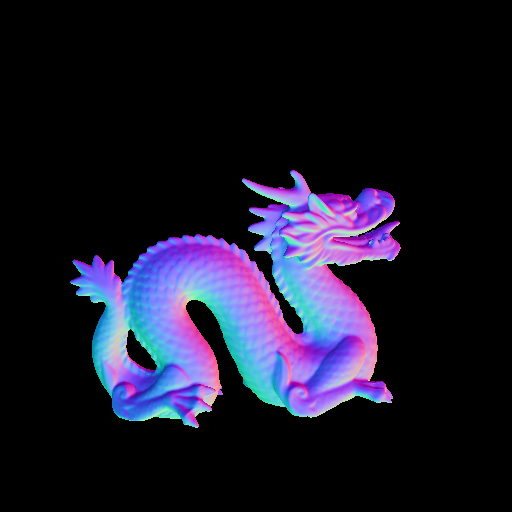
\includegraphics[width=\linewidth]{./Figures/svd-synthetic/no-noise/fancy_eval_22_groundtruth.png}
		\caption{GT}
	\end{subfigure}
	\begin{subfigure}[b]{0.32\linewidth}
		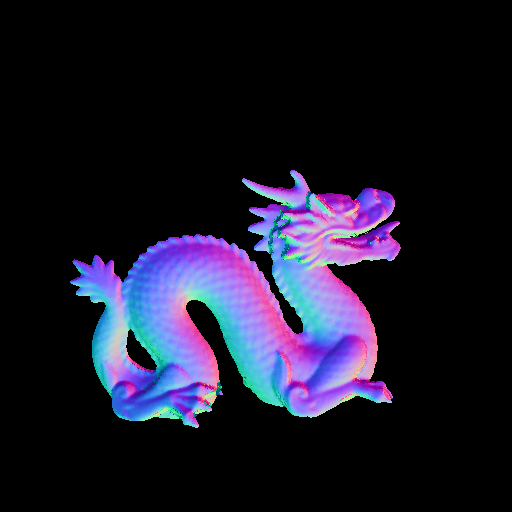
\includegraphics[width=\linewidth]{./Figures/svd-synthetic/no-noise/fancy_eval_22_normal_SVD.png}
		\caption{SVD}
	\end{subfigure}
	\begin{subfigure}[b]{0.32\linewidth}
		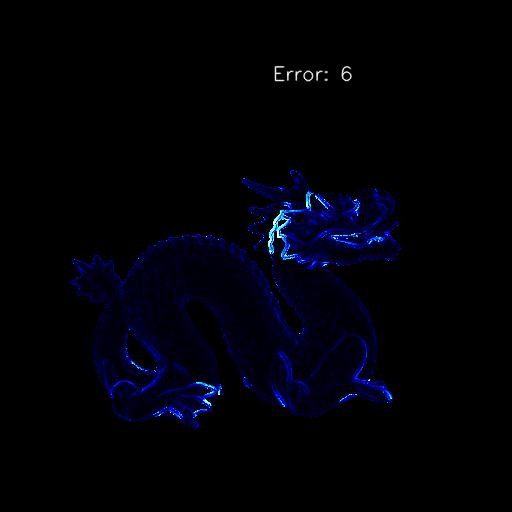
\includegraphics[width=\linewidth]{./Figures/svd-synthetic/no-noise/fancy_eval_22_error_SVD.png}
		\caption{Error}
	\end{subfigure}
	\begin{tikzpicture}
		\node[text width=0.1\textwidth] at (11,-1) {90};
		\node[inner sep=0pt] (input) at (8,-1)
		{
\includegraphics[width=.2\textwidth]{./Figures/colorscale_blue.png}};
		\node[text width=0.3\textwidth] at (7,-1) {Error: 0};
	\end{tikzpicture}
	
	\decoRule
	\caption{Normal map of a dragon object predicted by \textit{SVD}. k=1. (Resolution: $ 512\times 512 $) }
	\label{fig:svd-normal}
\end{figure}

\begin{figure}[th]
	\centering
	\captionsetup{width=\linewidth}
	\begin{subfigure}[b]{0.24\linewidth}
		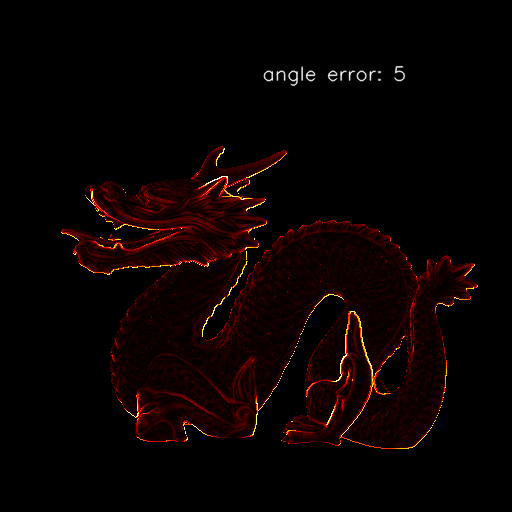
\includegraphics[width=\linewidth]{./Figures/svd-synthetic/k-compare/k1.png}
		\caption{$ k=1 $}
	\end{subfigure}
	\begin{subfigure}[b]{0.24\linewidth}
		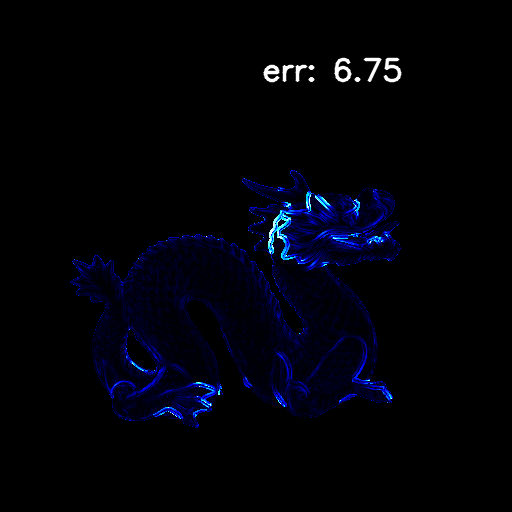
\includegraphics[width=\linewidth]{./Figures/svd-synthetic/k-compare/k2.png}
		\caption{$ k=2 $}
	\end{subfigure}
	\begin{subfigure}[b]{0.24\linewidth}
	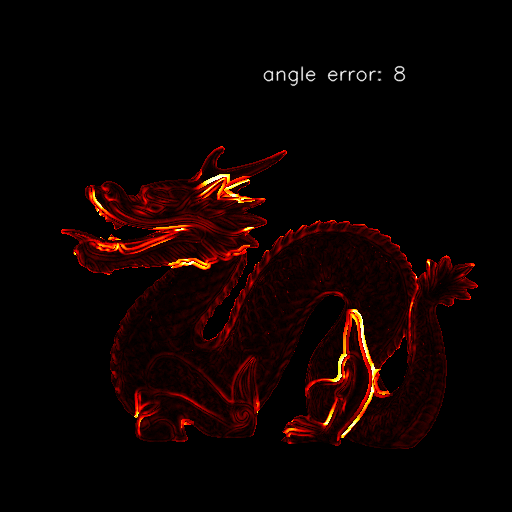
\includegraphics[width=\linewidth]{./Figures/svd-synthetic/k-compare/k3.png}
	\caption{$ k=3 $}
\end{subfigure}
	\begin{subfigure}[b]{0.24\linewidth}
	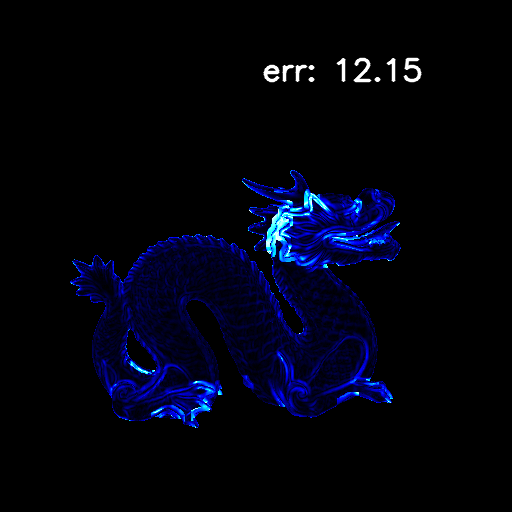
\includegraphics[width=\linewidth]{./Figures/svd-synthetic/k-compare/k4.png}
	\caption{$ k=4 $}
\end{subfigure}
	\begin{tikzpicture}
	\node[text width=0.1\textwidth] at (11,-1) {90};
	\node[inner sep=0pt] (input) at (8,-1)
	{
\includegraphics[width=.2\textwidth]{./Figures/colorscale_blue.png}};
	\node[text width=0.3\textwidth] at (7,-1) {Error: 0};
	\end{tikzpicture}
	\decoRule
	\caption{Error map of \textit{SVD} with different $ k $ values. (Resolution: $ 512\times 512 $) }
	\label{fig:svd-k-eval}
\end{figure}



\begin{figure}[H]
	\centering
	\captionsetup{width=\linewidth}
	\begin{subfigure}[b]{0.24\linewidth}
		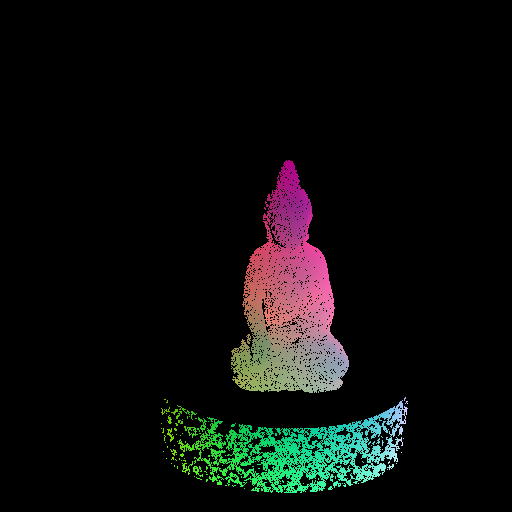
\includegraphics[width=\linewidth]{./Figures/svd-synthetic/noise/fancy_eval_0_point_cloud_noise.png}
		\caption{Vertex}
	\end{subfigure}
	\begin{subfigure}[b]{0.24\linewidth}
		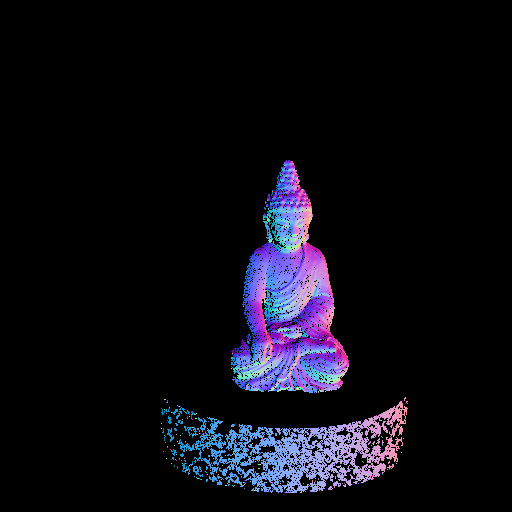
\includegraphics[width=\linewidth]{./Figures/svd-synthetic/noise/fancy_eval_0_groundtruth.png}
		\caption{GT}
	\end{subfigure}
	\begin{subfigure}[b]{0.24\linewidth}
		\includegraphics[width=\linewidth]{./Figures/svd-synthetic/noise/fancy_eval_0_normal_SVD.png}
		\caption{SVD}
	\end{subfigure}
	\begin{subfigure}[b]{0.24\linewidth}
		\includegraphics[width=\linewidth]{./Figures/svd-synthetic/noise/fancy_eval_0_error_SVD.png}
		\caption{Error}
	\end{subfigure}
	\begin{tikzpicture}
		\node[text width=0.1\textwidth] at (11,-1) {90};
		\node[inner sep=0pt] (input) at (8,-1)
		{\includegraphics[width=.2\textwidth]{./Figures/colorscale_blue.png}};
		\node[text width=0.3\textwidth] at (7,-1) {Error: 0};
	\end{tikzpicture}	
	\decoRule
	\caption{\textit{SVD} visual evaluation on a noised dragon model, $ k=1 $, noise factor $ \mu $=50. (Resolution: $ 512\times 512 $) }
	\label{fig:svd-noise}
\end{figure}

The SVD approach depends on a well-chosen neighborhood size $ k $. Figure \ref{fig:svd-k-eval} shows the evaluation for different $ k $ values. For $ k=1 $, the average angle error of the whole image is the smallest, most of the normals are close to the ground truth, but the outline edges, i.e., the areas where the surface normals have changed severely. In the $ k=2 $ case, the sharp edges are smoother and cause more error, such as the eye area of the dragon. Compared to the first case, the outline edge error is better. Most of the edge errors are reduced at $ k=2 $ because more neighbor points are included in the evaluation and the effect of outliers is reduced. However, in the area of the horn outline and the hindleg outline, the error becomes worse. In this case, most of the neighbors of these points are outliers.  With $ k=3 $ and $ k=4 $, the average angular errors increase further compared to $ k=2 $.

The performance of the neighborhood-based method is good enough for a well-chosen $ k $. However, in the case of a noisy point cloud as input, this approach fails because the noise does not satisfy the neighborhood assumption and also reduces the number of possible neighbors of each point for a fixed $ k $. See figure \ref{fig:svd-noise}.



\section{Visual Evaluation on GCNN}
A qualitative evaluation on object "dragon" is shown in Figure \ref{fig:gcnn-eval}. As shown in the figure, GCNN model achieved a mean angle error in 9 degrees on this dragon object. The image has an overall good performance on the whole object. A closer evaluation is shown in Figure \ref{fig:gcnn-eval-synthetic-zoom-in}, the normal accuracy especially good on the smooth surface, like the body area. In the same case, NOC model as shown in Figure \ref{fig:gcnn-eval-multi-model} has an overall worse normal than GCNN model in the smooth area. CNN model keeps the skip connection thus gives a sharper result than NOC model, however, the overall smooth part of the model is still worse than GCNN. Besides, the sharp area like the hindleg and the head area of dragon object, CNN model gives a much brighter error map (which means a higher angle error). Figure \ref{fig:gcnn-eval-more} shows more evaluation on GCNN model.

We can get a good result from GCNN model, but from model ``Washington" we still can see it lacks the sharpness in the detail area like the face and clothes area. 


A qualitative evaluation of the object \textit{Dragon} is shown in figure \ref{fig:gcnn-eval}. As can be seen in the figure, the \textit{GCNN} model achieves an average angular error of 9 degrees for this object. The image shows an overall good performance for the whole object. A more detailed evaluation can be seen in Figure \ref{fig:gcnn-eval-synthetic-zoom-in}, the normal accuracy is especially good on the smooth surface, such as the body area. In the same case, as shown in Figure \ref{fig:gcnn-eval-multi-model}, the \textit{NOC} model has an overall worse normal than the \textit{GCNN} model in the smooth area. The \textit{CNN} model retains the skip connection and thus yields a sharper result than the \textit{NOC} model, however, the smooth region of the model is still worse overall than the \textit{GCNN} model. In addition, the \textit{CNN} model yields a much brighter error map (implying a higher angular error) in the sharp regions such as the hind leg and the head region of the dragon object. Figure \ref{fig:gcnn-eval-more} shows further evaluation of the \textit{GCNN} model on other objects.
The \textit{GCNN} model gives a good result, but for the \textit{Washington} model there is still a lack of sharpness in the detail areas such as the face and clothing. 



%% GCNN-eval
\begin{figure}[H]
	\centering
	\captionsetup{width=\linewidth}
	\begin{subfigure}[b]{0.24\linewidth}
		\includegraphics[width=\linewidth]{./Figures/gcnn_synthetic/fancy_eval_7_img.png}
		\caption{Image}
	\end{subfigure}
	\begin{subfigure}[b]{0.24\linewidth}
		\includegraphics[width=\linewidth]{./Figures/gcnn_synthetic/fancy_eval_7_groundtruth.png}
		\caption{GT}
	\end{subfigure}
	\begin{subfigure}[b]{0.24\linewidth}
		\includegraphics[width=\linewidth]{./Figures/gcnn_synthetic/fancy_eval_7_normal_GCNN-GCNN.png}
		\caption{Predict}
	\end{subfigure}
	\begin{subfigure}[b]{0.24\linewidth}
		\includegraphics[width=\linewidth]{./Figures/gcnn_synthetic/fancy_eval_7_error_GCNN.png}
		\caption{Error}
	\end{subfigure}
	
	\begin{tikzpicture}
		\node[text width=0.1\textwidth] at (11,-1) {90};
		\node[inner sep=0pt] (input) at (8,-1)
		{\includegraphics[width=.2\textwidth]{./Figures/colorscale_blue.png}};
		\node[text width=0.3\textwidth] at (7,-1) {Error: 0};
	\end{tikzpicture}
	\decoRule
	\caption{GCNN visual evaluation. (Resolution: $ 128\times128 $)}
	\label{fig:gcnn-eval}
\end{figure}

%% GCNN zoom in eval
\begin{figure}[th]
	\centering
	\captionsetup{width=\linewidth}
	\begin{subfigure}[b]{0.18\linewidth}
		\includegraphics[width=\linewidth]{./Figures/gcnn_synthetic/eval_7_22_-8_normal.png}
	\end{subfigure}
	\begin{subfigure}[b]{0.18\linewidth}
		\includegraphics[width=\linewidth]{./Figures/gcnn_synthetic/eval_7_2_22_normal.png}
	\end{subfigure}
	\begin{subfigure}[b]{0.18\linewidth}
		\includegraphics[width=\linewidth]{./Figures/gcnn_synthetic/eval_7_32_12_normal.png}
	\end{subfigure}
	\begin{subfigure}[b]{0.18\linewidth}
		\includegraphics[width=\linewidth]{./Figures/gcnn_synthetic/eval_7_42_-28_normal.png}
	\end{subfigure}
	\begin{subfigure}[b]{0.18\linewidth}
		\includegraphics[width=\linewidth]{./Figures/gcnn_synthetic/eval_7_12_-48_normal.png}
	\end{subfigure}
	
	\begin{subfigure}[b]{0.18\linewidth}
		\includegraphics[width=\linewidth]{./Figures/gcnn_synthetic/eval_7_22_-8_error.png}
		\caption{Scale}
	\end{subfigure}
	\begin{subfigure}[b]{0.18\linewidth}
		\includegraphics[width=\linewidth]{./Figures/gcnn_synthetic/eval_7_2_22_error.png}
		\caption{Head}
	\end{subfigure}
	\begin{subfigure}[b]{0.18\linewidth}
		\includegraphics[width=\linewidth]{./Figures/gcnn_synthetic/eval_7_32_12_error.png}
		\caption{Foreleg}
	\end{subfigure}
	\begin{subfigure}[b]{0.18\linewidth}
		\includegraphics[width=\linewidth]{./Figures/gcnn_synthetic/eval_7_42_-28_error.png}
		\caption{Hindleg}
	\end{subfigure}
	\begin{subfigure}[b]{0.18\linewidth}
		\includegraphics[width=\linewidth]{./Figures/gcnn_synthetic/eval_7_12_-48_error.png}
		\caption{Tail}
	\end{subfigure}
	
	\decoRule
	\caption{Zoom in of some regions of Dragon object (GCNN models). (Resolution: $ 32\times32 $)}
	\label{fig:gcnn-eval-synthetic-zoom-in}
\end{figure}

%% compare to other models

%% GCNN zoom in eval
\begin{figure}[H]
	\centering
	\begin{subfigure}[b]{0.24\linewidth}
		\includegraphics[width=\linewidth]{./Figures/gcnn_synthetic/fancy_eval_7_groundtruth.png}
	\end{subfigure}
	\begin{subfigure}[b]{0.24\linewidth}
		\includegraphics[width=\linewidth]{./Figures/gcnn_synthetic/fancy_eval_7_normal_GCNN-GCNN.png}
	\end{subfigure}
	\begin{subfigure}[b]{0.24\linewidth}
		\includegraphics[width=\linewidth]{./Figures/gcnn_synthetic/fancy_eval_7_normal_GCNN-NOC.png}
	\end{subfigure}
	\begin{subfigure}[b]{0.24\linewidth}
		\includegraphics[width=\linewidth]{./Figures/gcnn_synthetic/fancy_eval_7_normal_GCNN-CNN.png}
	\end{subfigure}
	
	\begin{subfigure}[b]{0.24\linewidth}
		\includegraphics[width=\linewidth]{./Figures/gcnn_synthetic/fancy_eval_7_img.png}
		\caption{GT}
	\end{subfigure}
	\begin{subfigure}[b]{0.24\linewidth}
		\includegraphics[width=\linewidth]{./Figures/gcnn_synthetic/fancy_eval_7_error_GCNN-GCNN.png}
		\caption{GCNN}
	\end{subfigure}
	\begin{subfigure}[b]{0.24\linewidth}
		\includegraphics[width=\linewidth]{./Figures/gcnn_synthetic/fancy_eval_7_error_GCNN-NOC.png}
		\caption{NOC}
	\end{subfigure}
	\begin{subfigure}[b]{0.24\linewidth}
		\includegraphics[width=\linewidth]{./Figures/gcnn_synthetic/fancy_eval_7_error_GCNN-CNN.png}
		\caption{CNN}
	\end{subfigure}
	
	\decoRule
	\caption{Comparison of GCNN based models. (Resolution: $ 128\times 128 $)}
	\label{fig:gcnn-eval-multi-model}
\end{figure}


\section{Discussion on the Feature Maps in GCNN}

As shown in Figure \ref{fig:gcnn-cnn-feature map}, we visualize the feature maps of the last gated convolution layer in the first upsampling part for \textit{GCNN}, \textit{NOC} and \textit{CNN} models corresponding to the 128 feature maps with size $ 32\times 32 $ in width and height. 
The input data is also the same dragon object that we used for the normal visualization. For each feature map, we assign the minimum value to the leftmost color in the color bar and the maximum value to the rightmost color in the color bar. 
We want to discuss the difference of feature maps between these three models.

To see the result clearly, we use green hue to visualize the feature maps and use brightness to distinguish the scale of the values: White corresponds to 1, Black corresponds to 0, and the colors with green hue correspond to some values in between. 

\begin{figure}[H]
	\centering
	\captionsetup{width=\linewidth}
	\begin{subfigure}[b]{0.19\linewidth}
		\includegraphics[width=\linewidth]{./Figures/feature_map_gcnn/feature_map_normal_gcnn-cnn.png}
		\caption{Normal Map}
	\end{subfigure}
	\begin{subfigure}[b]{0.19\linewidth}
		\includegraphics[width=\linewidth]{./Figures/feature_map_gcnn/feature_map_gcnn-cnn_46.png}
		\caption{Feature Map}
	\end{subfigure}
	\begin{subfigure}[b]{0.19\linewidth}
		\includegraphics[width=\linewidth]{./Figures/feature_map_gcnn/feature_map_gcnn-cnn_11.png}
		\caption{Feature Map}
	\end{subfigure}
	\begin{subfigure}[b]{0.19\linewidth}
		\includegraphics[width=\linewidth]{./Figures/feature_map_gcnn/feature_map_gcnn-cnn_4.png}
		\caption{Feature Map}
	\end{subfigure}
	\begin{subfigure}[b]{0.19\linewidth}
		\includegraphics[width=\linewidth]{./Figures/feature_map_gcnn/feature_map_gcnn-cnn_2.png}
		\caption{Feature Map}
	\end{subfigure}
	
	\begin{tikzpicture}
		\node[text width=0.1\textwidth] at (11,-1) {1};
		\node[inner sep=0pt] (input) at (8,-1)
		{\includegraphics[width=.2\textwidth]{./Figures/colorscale_deepgreen.jpg}};
		\node[text width=0.3\textwidth] at (7,-1) {Value: 0};
	\end{tikzpicture}
	\decoRule
	\caption{Some of feature maps of CNN model in up-sampling part on resolution $ 32\times32 $}
	\label{fig:detail-feature-maps}
\end{figure}



\begin{figure}[H]
	\centering
	\captionsetup{width=\linewidth}
	\begin{subfigure}[b]{0.19\linewidth}
		\includegraphics[width=\linewidth]{./Figures/feature_map_gcnn/feature_map_out_gcnn-noc.png}
		\caption{Normal Map}
	\end{subfigure}
	\begin{subfigure}[b]{0.19\linewidth}
		\includegraphics[width=\linewidth]{./Figures/feature_map_gcnn/feature_map_gcnn-noc_39.png}
		\caption{Feature Map}
	\end{subfigure}
	\begin{subfigure}[b]{0.19\linewidth}
		\includegraphics[width=\linewidth]{./Figures/feature_map_gcnn/feature_map_gcnn-noc_45.png}
		\caption{Feature Map}
	\end{subfigure}
	\begin{subfigure}[b]{0.19\linewidth}
		\includegraphics[width=\linewidth]{./Figures/feature_map_gcnn/feature_map_gcnn-noc_93.png}
		\caption{Feature Map}
	\end{subfigure}
	\begin{subfigure}[b]{0.19\linewidth}
		\includegraphics[width=\linewidth]{./Figures/feature_map_gcnn/feature_map_gcnn-noc_104.png}
		\caption{Feature Map}
	\end{subfigure}
	
	\begin{tikzpicture}
		\node[text width=0.1\textwidth] at (11,-1) {1};
		\node[inner sep=0pt] (input) at (8,-1)
		{\includegraphics[width=.2\textwidth]{./Figures/colorscale_deepgreen.jpg}};
		\node[text width=0.3\textwidth] at (7,-1) {Value: 0};
	\end{tikzpicture}
	\decoRule
	\caption{Some of feature maps of NOC model in up-sampling part on resolution $ 32\times32 $}
	\label{fig:detail-feature-maps}
\end{figure}




\begin{figure}[H]
	\centering
	\captionsetup{width=\linewidth}
	\begin{subfigure}[b]{0.19\linewidth}
		\includegraphics[width=\linewidth]{./Figures/feature_map_gcnn/feature_map_out_gcnn-gcnn.png}
		\caption{Normal Map}
	\end{subfigure}
	\begin{subfigure}[b]{0.19\linewidth}
		\includegraphics[width=\linewidth]{./Figures/feature_map_gcnn/feature_map_gcnn-gcnn_4.png}
		\caption{Feature Map}
	\end{subfigure}
	\begin{subfigure}[b]{0.19\linewidth}
		\includegraphics[width=\linewidth]{./Figures/feature_map_gcnn/feature_map_gcnn-gcnn_5.png}
		\caption{Feature Map}
	\end{subfigure}
	\begin{subfigure}[b]{0.19\linewidth}
		\includegraphics[width=\linewidth]{./Figures/feature_map_gcnn/feature_map_gcnn-gcnn_15.png}
		\caption{Feature Map}
	\end{subfigure}
	\begin{subfigure}[b]{0.19\linewidth}
		\includegraphics[width=\linewidth]{./Figures/feature_map_gcnn/feature_map_gcnn-gcnn_127.png}
		\caption{Feature Map}
	\end{subfigure}
	
	\begin{tikzpicture}
		\node[text width=0.1\textwidth] at (11,-1) {1};
		\node[inner sep=0pt] (input) at (8,-1)
		{\includegraphics[width=.2\textwidth]{./Figures/colorscale_deepgreen.jpg}};
		\node[text width=0.3\textwidth] at (7,-1) {Value: 0};
	\end{tikzpicture}
	\decoRule
	\caption{Some of feature maps of GCNN model in up-sampling part on resolution $ 32\times32 $}
	\label{fig:detail-feature-maps}
\end{figure}

\begin{figure}[H]
		\centering
		\captionsetup{width=\linewidth}
		\begin{minipage}{0.32\linewidth}
				\begin{subfigure}[t]{0.45\linewidth}
					\includegraphics[width=\linewidth]{./Figures/feature_map_gcnn/feature_map_gcnn-cnn_113.png}
				\end{subfigure}
				\begin{subfigure}[t]{0.45\linewidth}
					\includegraphics[width=\linewidth]{./Figures/feature_map_gcnn/feature_map_gcnn-cnn_102.png}
				\end{subfigure}
			
				\begin{subfigure}[t]{0.45\linewidth}
					\includegraphics[width=\linewidth]{./Figures/feature_map_gcnn/feature_map_gcnn-cnn_65.png}
					\caption{CNN}
				\end{subfigure}
				\begin{subfigure}[t]{0.45\linewidth}
				\includegraphics[width=\linewidth]{./Figures/feature_map_gcnn/feature_map_gcnn-cnn_28.png}
				\end{subfigure}
		\end{minipage}
		\begin{minipage}{0.32\linewidth}
				\begin{subfigure}[t]{0.45\linewidth}
					\includegraphics[width=\linewidth]{./Figures/feature_map_gcnn/feature_map_gcnn-noc_7.png}
				\end{subfigure}
				\begin{subfigure}[t]{0.45\linewidth}
					\includegraphics[width=\linewidth]{./Figures/feature_map_gcnn/feature_map_gcnn-noc_25.png}
				\end{subfigure}
			
				\begin{subfigure}[t]{0.45\linewidth}
					\includegraphics[width=\linewidth]{./Figures/feature_map_gcnn/feature_map_gcnn-noc_11.png}
					\caption{NOC}
				\end{subfigure}
				\begin{subfigure}[t]{0.45\linewidth}
				\includegraphics[width=\linewidth]{./Figures/feature_map_gcnn/feature_map_gcnn-noc_127.png}
				\end{subfigure}
			
		\end{minipage}
		\begin{minipage}{0.32\linewidth}
				\begin{subfigure}[t]{0.45\linewidth}
					\includegraphics[width=\linewidth]{./Figures/feature_map_gcnn/feature_map_gcnn-gcnn_1.png}
				\end{subfigure}
				\begin{subfigure}[t]{0.45\linewidth}
					\includegraphics[width=\linewidth]{./Figures/feature_map_gcnn/feature_map_gcnn-gcnn_9.png}
				\end{subfigure}
			
				\begin{subfigure}[t]{0.45\linewidth}
					\includegraphics[width=\linewidth]{./Figures/feature_map_gcnn/feature_map_gcnn-gcnn_24.png}
					\caption{GCNN}
				\end{subfigure}
					\begin{subfigure}[t]{0.45\linewidth}
				\includegraphics[width=\linewidth]{./Figures/feature_map_gcnn/feature_map_gcnn-gcnn_75.png}
				\end{subfigure}
			
		\end{minipage}
	
		\begin{tikzpicture}
			\node[text width=0.1\textwidth] at (11,-1) {1};
			\node[inner sep=0pt] (input) at (8,-1)
			{\includegraphics[width=.2\textwidth]{./Figures/colorscale_deepgreen.jpg}};
			\node[text width=0.3\textwidth] at (7,-1) {Value: 0};
		\end{tikzpicture}
		\decoRule
		\caption{Some of feature maps of GCNN model in up-sampling part on resolution $ 32\times32 $}
		\label{fig:global-feature-maps}
\end{figure}





From the CNN feature maps, we can see that the high-value areas usually represent more than one in a single feature map. Many of them have more than two bright areas. 
In the GCNN feature maps, the bright areas are usually concentrated in only one area or even one point. When we map the bright areas onto the original image, they correspond to the dense, sharp areas, such as the mouse, horn, or tail of the kite object, which are usually the most difficult areas for the normal estimation task. We assume that these feature maps with few bright areas or only one bright area are the detail feature maps from which sharp edges can be inferred. Based on this assumption, we can say that the gated convolution layer describes the detail features more accurately compared to the standard convolution layer because the brightness regions are smaller. Most GCNN feature maps have only one bright pixel with a few green pixels, while CNN feature maps have more bright pixels with many dark pixels around the image. This accurate feature extraction gives our GCNN model better performance in the detailed areas.

Second, with the GCNN model, we found that some feature maps have very uniformly bright areas across the entire object. They are either dark overall or bright overall. Nevertheless, these feature maps differ from the detail feature maps with only a few pixels with high values (brightness), but most other pixels with relatively low values. We suspect that these uniformly distributed feature maps are the global feature maps that provide an overview of the objects for rough prediction. Thus, they can cooperate with detailed feature maps to further refine the prediction. This is also true for the NOC model since it does not have skip connections and most of the feature maps are global feature maps, so the corresponding normal maps predicted by the NOC model are coarser than those of the GCNN model. For the CNN model, there are also global feature maps, but most of them are incomplete because either the tails or the paws are missing. 
These missing areas are usually found in the detail feature maps. This also explains why the CNN detail feature maps have several bright areas in their detail feature maps. The detail feature maps and the global feature maps are mixed together. And this unclear feature map extractor leads to a decrease in performance in normal estimation tasks.




\newpage 
\section{Visual Evaluation on Trip-Net}
In the approach that uses an illuminated, calibrated RGBD image, the task is performed by the Trip-Net presented in \ref{sec:trip-net}. Based on illumination and geometry information, the Trip-Net achieves a sharper and more accurate result compared to the GCNN model.


%% TripNet-eval
\begin{figure}[H]
	\centering
	\captionsetup{width=\linewidth}
	\begin{subfigure}[b]{0.24\linewidth}
		\includegraphics[width=\linewidth]{./Figures/gcnn_synthetic/fancy_eval_7_img.png}
		\caption{Image}
	\end{subfigure}
	\begin{subfigure}[b]{0.24\linewidth}
		\includegraphics[width=\linewidth]{./Figures/gcnn_synthetic/fancy_eval_7_groundtruth.png}
		\caption{GT}
	\end{subfigure}
	\begin{subfigure}[b]{0.24\linewidth}
		\includegraphics[width=\linewidth]{./Figures/gcnn_synthetic/fancy_eval_7_normal_an2-8-1000.png}
		\caption{Predict}
	\end{subfigure}
	\begin{subfigure}[b]{0.24\linewidth}
		\includegraphics[width=\linewidth]{./Figures/gcnn_synthetic/fancy_eval_7_error_an2-8-1000.png}
		\caption{Error}
	\end{subfigure}
	
	\begin{tikzpicture}
		\node[text width=0.1\textwidth] at (11,-1) {90};
		\node[inner sep=0pt] (input) at (8,-1)
		{\includegraphics[width=.2\textwidth]{./Figures/colorscale_blue.png}};
		\node[text width=0.3\textwidth] at (7,-1) {Error: 0};
	\end{tikzpicture}
	\decoRule
	\caption{Trip-Net visual evaluation on resolution $ 128\times128 $}
	\label{fig:trip-eval}
\end{figure}
The qualitative evaluation is shown in Figure \ref{fig:trip-eval}. To show the effectiveness of the added illuminated information, the training settings are exactly the same for all models. We also use the same inputs as for the GCNN evaluation. The error of the Trip-Net is $ 6^\circ $, and that of the GCNN is $ 9^\circ $. 

%% tripNet zoom in eval
\begin{figure}[H]
	\centering
	\captionsetup{width=\linewidth}
	\begin{subfigure}[b]{0.18\linewidth}
		\includegraphics[width=\linewidth]{./Figures/trip_net_zoom_in/eval_7_22_-8_normal.png}
	\end{subfigure}
	\begin{subfigure}[b]{0.18\linewidth}
		\includegraphics[width=\linewidth]{./Figures/trip_net_zoom_in/eval_7_2_22_normal.png}
	\end{subfigure}
	\begin{subfigure}[b]{0.18\linewidth}
		\includegraphics[width=\linewidth]{./Figures/trip_net_zoom_in/eval_7_32_12_normal.png}
	\end{subfigure}
	\begin{subfigure}[b]{0.18\linewidth}
		\includegraphics[width=\linewidth]{./Figures/trip_net_zoom_in/eval_7_42_-28_normal.png}
	\end{subfigure}
	\begin{subfigure}[b]{0.18\linewidth}
		\includegraphics[width=\linewidth]{./Figures/trip_net_zoom_in/eval_7_12_-48_normal.png}
	\end{subfigure}
	
	\begin{subfigure}[b]{0.18\linewidth}
		\includegraphics[width=\linewidth]{./Figures/trip_net_zoom_in/eval_7_22_-8_error.png}
		\caption{Scale}
	\end{subfigure}
	\begin{subfigure}[b]{0.18\linewidth}
		\includegraphics[width=\linewidth]{./Figures/trip_net_zoom_in/eval_7_2_22_error.png}
		\caption{Head}
	\end{subfigure}
	\begin{subfigure}[b]{0.18\linewidth}
		\includegraphics[width=\linewidth]{./Figures/trip_net_zoom_in/eval_7_32_12_error.png}
		\caption{Foreleg}
	\end{subfigure}
	\begin{subfigure}[b]{0.18\linewidth}
		\includegraphics[width=\linewidth]{./Figures/trip_net_zoom_in/eval_7_42_-28_error.png}
		\caption{Hindleg}
	\end{subfigure}
	\begin{subfigure}[b]{0.18\linewidth}
		\includegraphics[width=\linewidth]{./Figures/trip_net_zoom_in/eval_7_12_-48_error.png}
		\caption{Tail}
	\end{subfigure}
	
	\decoRule
	\caption{Zoom in of detail regions ($ 32\times32 $) of \textit{Dragon} object (Trip-Net).}
	\label{fig:tripnet-eval-synthetic-zoom-in}
\end{figure}

As can be seen in the Figure \ref{fig:tripnet-eval-synthetic-zoom-in}, the scale of the dragon's body is much easier to see and is also closer to the ground truth. The head region provides a sharper edge prediction. All five sampled zoom-in regions in Trip-Net have better performance than GCNN. 


Figure \ref{fig:tripnet-fusion-eval} compares different fusion times on the Trip-Net model. It can be seen that the F1 with one fusion and F2 with two fusions models do not perform better compared to the GCNN model, which means that the illuminated information does not work when we consider only the lower resolution feature maps. The F3 model with three fusions and the F4 model with four fusions provide a much better result and also outperform the GCNN model. In these two fusion models, the high-resolution features are included. We can observe the dragon scale in the figures, it is much sharper in F3 and F4.

%% F1-F4 eval

\begin{figure}
	\centering
	\captionsetup{width=\linewidth}
	\begin{subfigure}[b]{0.18\linewidth}
		\includegraphics[width=\linewidth]{./Figures/gcnn_synthetic/fancy_eval_7_groundtruth.png}
	\end{subfigure}
	\begin{subfigure}[b]{0.18\linewidth}
		\includegraphics[width=\linewidth]{./Figures/gcnn_synthetic/fancy_eval_7_normal_f1.png}
	\end{subfigure}
	\begin{subfigure}[b]{0.18\linewidth}
		\includegraphics[width=\linewidth]{./Figures/gcnn_synthetic/fancy_eval_7_normal_f2.png}
	\end{subfigure}
	\begin{subfigure}[b]{0.18\linewidth}
		\includegraphics[width=\linewidth]{./Figures/gcnn_synthetic/fancy_eval_7_normal_f3.png}
	\end{subfigure}
	\begin{subfigure}[b]{0.18\linewidth}
		\includegraphics[width=\linewidth]{./Figures/gcnn_synthetic/fancy_eval_7_normal_f4.png}
	\end{subfigure}
	
	
	\begin{subfigure}[b]{0.18\linewidth}
		\includegraphics[width=\linewidth]{./Figures/gcnn_synthetic/fancy_eval_7_img.png}
		\caption{GT}
	\end{subfigure}
	\begin{subfigure}[b]{0.18\linewidth}
		\includegraphics[width=\linewidth]{./Figures/gcnn_synthetic/fancy_eval_7_error_f1.png}
		\caption{F1}
	\end{subfigure}
	\begin{subfigure}[b]{0.18\linewidth}
		\includegraphics[width=\linewidth]{./Figures/gcnn_synthetic/fancy_eval_7_error_f2.png}
		\caption{F2}
	\end{subfigure}
	\begin{subfigure}[b]{0.18\linewidth}
		\includegraphics[width=\linewidth]{./Figures/gcnn_synthetic/fancy_eval_7_error_f3.png}
		\caption{F3}
	\end{subfigure}
	\begin{subfigure}[b]{0.18\linewidth}
		\includegraphics[width=\linewidth]{./Figures/gcnn_synthetic/fancy_eval_7_error_f4.png}
		\caption{F4}
	\end{subfigure}
	
	\decoRule
	\caption{Comparison between different fusion times on Trip-Net Architecture ($ 128\times128 $). }
	\label{fig:tripnet-fusion-eval}
\end{figure}




\section{Trining on Higher Resolution}
We also trained our models on a higher resolution dataset with $ 512 \times 512 $ in width and height for each scene. Higher resolution data provides more information about surface features using the same model compared to lower resolutions. The advantage is that if we extract a fixed size patch from the normal map, say $32\times32$, it may correspond to a hind leg of the dragon object at a resolution of $128 \times 128$ scene, but at a resolution of $512\times 512$ scene, it may only correspond to a toe. Thus, if we still use the same kernel size in the network for the same data set (as in $ 3\times 3 $), the higher the resolution, the smaller the corresponding surface area. 
Thus, for the higher resolution, the surface becomes smoother and the surface normal can be computed more easily in a fixed size of area compare to lower resolution. This is a good thing. Because then we may only need to use these $ 32\ times 32 $ points to calculate a toe in an image with $ 512\ times512 $ resolution. But in an image with a resolution of $ 128\times128 $, the same area $ 32\times32 $ could correspond to the entire hind leg of the dragon object. In other words. Thus, the higher resolution helps the model to compute a more accurate normal map. 


%% 5 degree metric
\begin{table}[H]
	\centering
	\captionsetup{width=\linewidth}
	\begin{tabular}{l | l l l }
		\toprule
		\tabhead{Metrics} & \tabhead{SVD} & \tabhead{GCNN} & \tabhead{Trip-Net} \\
		\midrule
		Mean  					& 8.88 & 5.82 & 5.33 \\ 
		\hline
		Median					& 3.66 & 3.98 & 3.67 \\ 
		\hline
		$ 5^\circ $ 			& 0.63 & 0.63 & 0.66 \\
		\hline
		$ 11.5^\circ $ 			& 0.79 & 0.89 & 0.91 \\
		\hline
		$ 22.5^\circ $ 			& 0.89 & 0.97 & 0.97 \\
		\hline
		$ 30^\circ $ 			& 0.92 & 0.98 & 0.99 \\
		\bottomrule
	\end{tabular}
	\caption{High resolution dataset evaluation of SVD, GCNN and Trip-Net models on 6 different metrics based on 100 test scenes. (Resolution: $ 512\times512 $)}	
	\label{tab:high_resolution_eval}
\end{table}

Since our model is a fully convolutional network, the architecture remains exactly the same on the high-resolution dataset. We use the same settings and the same model for training on a $ 512\times512 $ resolution dataset. Training with the high-resolution network takes longer, but results in a lower angular error. 



%% high resolution trip-net visualization
\begin{figure}[th]
	\centering
	\captionsetup{width=\linewidth}
	\begin{subfigure}[b]{0.48\linewidth}
		\includegraphics[width=\linewidth]{./Figures/comparison_512/fancy_eval_11_normal_Trip-Net-512.png}
		\caption{Trip-Net}
	\end{subfigure}
	\begin{subfigure}[b]{0.48\linewidth}
		\includegraphics[width=\linewidth]{./Figures/comparison_512/fancy_eval_11_groundtruth.png}
		\caption{GT}
	\end{subfigure}
	
	
	\begin{subfigure}[b]{0.32\linewidth}
		\includegraphics[width=\linewidth]{./Figures/comparison_512/fancy_eval_11_point_cloud_noise.png}
		\caption{Input}
	\end{subfigure}
	\begin{subfigure}[b]{0.32\linewidth}
		\includegraphics[width=\linewidth]{./Figures/comparison_512/fancy_eval_11_img.png}
		\caption{Image}
	\end{subfigure}
	\begin{subfigure}[b]{0.32\linewidth}
		\includegraphics[width=\linewidth]{./Figures/comparison_512/fancy_eval_11_error_Trip-Net-512.png}
		\caption{Error}
	\end{subfigure}
	
	\begin{tikzpicture}
		\node[text width=0.1\textwidth] at (11,-1) {90};
		\node[inner sep=0pt] (input) at (8,-1)
		{\includegraphics[width=.2\textwidth]{./Figures/colorscale_blue.png}};
		\node[text width=0.3\textwidth] at (7,-1) {Error: 0};
	\end{tikzpicture}
	\decoRule
	\caption{Trip-Net visual evaluation on high resolution dataset $ 512 \times 512 $.}
	\label{fig:trip-eval-high-resolution}
\end{figure}







A quantitative evaluation is shown in Table \ref{tab:high_resolution_eval}. It follows the same performance ranking compared to lower resolutions, i.e. GCNN is better than the SVD approach and Trip-Net is slightly better than GCNN. The accuracy is 99\% in the $30^\circ $ metric. In the average error metric, the error is $ 5^\circ $.  A qualitative evaluation is shown in Figure \ref{fig:trip-eval-high-resolution}. We use a figure object with smooth regions (belly and arm) and highly detailed regions with sharp surfaces (the uneven surface of the stone table) for the evaluation. Our models yield a $ 5^\circ $ in the middle degree of the metric. 

A comparison with other models is shown in Figure \ref{fig:trip-eval-compare}. Note that we use the same dragon object (with slightly shifted location since they were collected at different times in the high-resolution dataset) for the assessment to allow a coherent comparison with the low-resolution dataset. The \textit{SVD} approach yields a good result ($8.88^\circ $ in the average degree metric). As mentioned earlier, the surfaces are relatively smoother when we keep the same window size for normal inference. In the high-resolution scenes, the percentage of missing pixels in a fixed window is the same as in the low-resolution scenes, but the remaining valid pixels in the same window size are on a relatively flat plane and are therefore good enough for accurate normal inference. However, as expected, we can still see the high-level error in the sharp edges of the dragon object, such as the horns and the hind leg areas, as shown in Figure \ref{fig:trip-eval-compare}.



%& trip-net evaluation with other models

\begin{figure}[th]
	\centering
	\captionsetup{width=\linewidth}
	\begin{subfigure}[b]{0.24\linewidth}
		\includegraphics[width=\linewidth]{./Figures/comparison_512/fancy_eval_14_groundtruth.png}
	\end{subfigure}
	\begin{subfigure}[b]{0.24\linewidth}
		\includegraphics[width=\linewidth]{./Figures/comparison_512/fancy_eval_14_normal_SVD.png}
	\end{subfigure}
	\begin{subfigure}[b]{0.24\linewidth}
		\includegraphics[width=\linewidth]{./Figures/comparison_512/fancy_eval_14_normal_NNNN-512.png}
	\end{subfigure}
	\begin{subfigure}[b]{0.24\linewidth}
		\includegraphics[width=\linewidth]{./Figures/comparison_512/fancy_eval_14_normal_Trip-Net-512.png}
	\end{subfigure}
	
	
	\begin{subfigure}[b]{0.24\linewidth}
		\includegraphics[width=\linewidth]{./Figures/comparison_512/fancy_eval_14_img.png}
		\caption{GT}
	\end{subfigure}
	\begin{subfigure}[b]{0.24\linewidth}
		\includegraphics[width=\linewidth]{./Figures/comparison_512/fancy_eval_14_error_SVD.png}
		\caption{SVD}
	\end{subfigure}
	\begin{subfigure}[b]{0.24\linewidth}
		\includegraphics[width=\linewidth]{./Figures/comparison_512/fancy_eval_14_error_NNNN-512.png}
		\caption{GCNN}
	\end{subfigure}
	\begin{subfigure}[b]{0.24\linewidth}
		\includegraphics[width=\linewidth]{./Figures/comparison_512/fancy_eval_14_error_Trip-Net-512.png}
		\caption{Trip-Net}
	\end{subfigure}
	\decoRule
	\caption{Comparison on high resolution dataset ($ 512\times 512 $).}
	\label{fig:trip-eval-compare}
\end{figure}


\section{Training on Real-Dataset}
We also applied our model to a dataset acquired with a structured light scanner in our laboratory to test the applicability of our model to the real dataset. For the approach based on geometry information, we directly use the GCNN model trained on synthetic datasets since it only needs the depth map as input and the scenarios of the two datasets are the same. For the approach based on illuminated calibrated RGB-D images, the model needs to be refined based on the real dataset because the light intensity, position, and camera matrix are different. We have refined the Trip-Net based on a pre-trained GCNN model with the same settings in previous experiments.


\begin{table}[H]
	\centering
	\captionsetup{width=\linewidth}
	\begin{tabular}{l | l l l }
		\toprule
		\tabhead{Metrics} & \tabhead{SVD} & \tabhead{GCNN} & \tabhead{Trip-Net} \\
		\midrule
		Mean  					& 8.20 & 8.74 & \textbf{8.09}\\ 
		\hline
		Median					& \textbf{4.87} & 5.70 & 5.00 \\ 
		\hline
		$ 5^\circ $ 			& \textbf{0.51} & 0.44 & 0.50 \\
		\hline
		$ 11.5^\circ $ 			& 0.79 & 0.79 & \textbf{0.81} \\
		\hline
		$ 22.5^\circ $ 			& 0.93 & 0.93 & \textbf{0.94} \\
		\hline
		$ 30^\circ $ 			& 0.96 & 0.96 & 0.96 \\
		\bottomrule
	\end{tabular}
	\caption{Evaluation of SVD, GCNN and Trip-Net models on 6 different metrics based on 100 test scenes in Real-Dataset.}	
	\label{tab:real_eval}
\end{table}


We do not have a ground truth for evaluation in the Real-Dataset. But if we look directly at the visualization in Figure \ref{fig:trip-eval-real}, we can see that the Trip-Net approach is well able to ``enhance'' the missing pixels in the scenes and also gives a sharp result. The wrinkles on the clothes are detectable and even countable. Figure \ref{fig:real_eval_compare} compares the trip net with other approaches.


However, we also noticed that the large holes in the base level are preserved in the Normal Maps. These large holes correspond to the shiny and dark texture regions that are often present in the depth map captured by the scanners. Since these large holes are only related to specific feature areas and also have irregular shapes, we did not simulate this type of noise in the synthetic dataset, but only with a sparse binary mask. Therefore, our models could not fill in missing large holes in the estimated normal map. Further work on this topic could be to find a way to generate a very similar depth map noise to obtain a more robust training dataset. 

\begin{figure}[th]
	\centering
	\captionsetup{width=\linewidth}
	\begin{subfigure}[b]{0.32\linewidth}
		\includegraphics[width=\linewidth]{./Figures/comparison_real/fancy_eval_20_groundtruth.png}
		\caption{GT}
	\end{subfigure}
	\begin{subfigure}[b]{0.32\linewidth}
	\includegraphics[width=\linewidth]{./Figures/comparison_real/fancy_eval_20_normal_An2_no_mask.png}
	\caption{Trip-Net}
	\end{subfigure}
	\begin{subfigure}[b]{0.32\linewidth}
		\includegraphics[width=\linewidth]{./Figures/comparison_real/fancy_eval_20_normal_An2-real-resume-616.png}
		\caption{Trip-Net (No-Mask)}
	\end{subfigure}
	
	\begin{subfigure}[b]{0.32\linewidth}
		\includegraphics[width=\linewidth]{./Figures/comparison_real/fancy_eval_20_point_cloud_noise.png}
		\caption{Input}
	\end{subfigure}
	\begin{subfigure}[b]{0.32\linewidth}
		\includegraphics[width=\linewidth]{./Figures/comparison_real/fancy_eval_22_img.png}
		\caption{Image}
	\end{subfigure}
	\begin{subfigure}[b]{0.32\linewidth}
		\includegraphics[width=\linewidth]{./Figures/comparison_real/fancy_eval_22_error_An2-real-resume.png}
		\caption{Error}
	\end{subfigure}
	
	\begin{tikzpicture}
		\node[text width=0.1\textwidth] at (11,-1) {90};
		\node[inner sep=0pt] (input) at (8,-1)
		{\includegraphics[width=.2\textwidth]{./Figures/colorscale_blue.png}};
		\node[text width=0.3\textwidth] at (7,-1) {Error: 0};
	\end{tikzpicture}
	\decoRule
	\caption{Real Dataset ($ 512\times 512 $) evaluation (Trip-Net)}
	\label{fig:trip-eval-real}
\end{figure}




%% real eval comparison
\begin{figure}[th]
	\centering
	\captionsetup{width=\linewidth}
	\begin{subfigure}[b]{0.2\linewidth}
		\includegraphics[width=\linewidth]{./Figures/comparison_real/fancy_eval_0_groundtruth.png}
	\end{subfigure}
	\begin{subfigure}[b]{0.2\linewidth}
		\includegraphics[width=\linewidth]{./Figures/comparison_real/fancy_eval_0_normal_SVD.png}
	\end{subfigure}
	\begin{subfigure}[b]{0.2\linewidth}
		\includegraphics[width=\linewidth]{./Figures/comparison_real/fancy_eval_0_normal_NNNN-512.png}
	\end{subfigure}
	\begin{subfigure}[b]{0.2\linewidth}
		\includegraphics[width=\linewidth]{./Figures/comparison_real/fancy_eval_0_normal_An2-real-resume.png}
	\end{subfigure}
	
	
	\begin{subfigure}[b]{0.2\linewidth}
		\includegraphics[width=\linewidth]{./Figures/comparison_real/00008.image0.png}
		\caption{GT}
	\end{subfigure}
	\begin{subfigure}[b]{0.2\linewidth}
		\includegraphics[width=\linewidth]{./Figures/comparison_real/fancy_eval_0_error_SVD.png}
		\caption{SVD}
	\end{subfigure}	
	\begin{subfigure}[b]{0.2\linewidth}
		\includegraphics[width=\linewidth]{./Figures/comparison_real/fancy_eval_0_error_NNNN-512.png}
		\caption{GCNN}
	\end{subfigure}
	\begin{subfigure}[b]{0.2\linewidth}
		\includegraphics[width=\linewidth]{./Figures/comparison_real/fancy_eval_0_error_An2-real-resume.png}
		\caption{Trip-Net}
	\end{subfigure}	
	\decoRule
	\caption{Real dataset ($ 512\times 512 $) comparison.}
	\label{fig:real_eval_compare}
\end{figure}
 
% Chapter Template

\chapter{Conclusion} % Main chapter title

\label{ch:06} % Change X to a consecutive number; for referencing this chapter elsewhere, use \ref{ChapterX}

%----------------------------------------------------------------------------------------
%	SECTION 1
%----------------------------------------------------------------------------------------
Gated convolution neural network... 

%----------------------------------------------------------------------------------------
%	THESIS CONTENT - APPENDICES
%----------------------------------------------------------------------------------------

\appendix % Cue to tell LaTeX that the following "chapters" are Appendices

% Include the appendices of the thesis as separate files from the Appendices folder
% Uncomment the lines as you write the Appendices

% Appendix A

\chapter{Dataset} % Main appendix title

\label{AppendixA} % For referencing this appendix elsewhere, use \ref{AppendixA}

%% dataset a
\newpage 
\begin{figure}
	\centering
	\captionsetup{width=\linewidth}
	\begin{subfigure}[b]{0.23\linewidth}
		\includegraphics[width=\linewidth]{./Figures/train-dataset/00.apoll.png}
		\caption{apoll}
	\end{subfigure}
	\begin{subfigure}[b]{0.23\linewidth}
		\includegraphics[width=\linewidth]{./Figures/train-dataset/01.arm.png}
		\caption{arm}
	\end{subfigure}
	\begin{subfigure}[b]{0.23\linewidth}
		\includegraphics[width=\linewidth]{./Figures/train-dataset/02.armadillo.png}
		\caption{armadillo}
	\end{subfigure}
	\begin{subfigure}[b]{0.23\linewidth}
		\includegraphics[width=\linewidth]{./Figures/train-dataset/03.bearded-guy.png}
		\caption{bearded-guy}
	\end{subfigure}
	
	\begin{subfigure}[b]{0.23\linewidth}
		\includegraphics[width=\linewidth]{./Figures/train-dataset/04.bronze-sculpture.png}
		\caption{bronze-sculpture}
	\end{subfigure}
	\begin{subfigure}[b]{0.23\linewidth}
		\includegraphics[width=\linewidth]{./Figures/train-dataset/05.bunny.png}
		\caption{bunny}
	\end{subfigure}
	\begin{subfigure}[b]{0.23\linewidth}
		\includegraphics[width=\linewidth]{./Figures/train-dataset/06.car-engine.png}
		\caption{car-engine}
	\end{subfigure}
	\begin{subfigure}[b]{0.23\linewidth}
		\includegraphics[width=\linewidth]{./Figures/train-dataset/07.cat.png}
		\caption{cat}
	\end{subfigure}
	
	\begin{subfigure}[b]{0.23\linewidth}
		\includegraphics[width=\linewidth]{./Figures/train-dataset/08.pergolesi-side-chair.png}
		\caption{side-chair}
	\end{subfigure}
	\begin{subfigure}[b]{0.23\linewidth}
		\includegraphics[width=\linewidth]{./Figures/train-dataset/09.chair2.png}
		\caption{chair2}
	\end{subfigure}
	\begin{subfigure}[b]{0.23\linewidth}
		\includegraphics[width=\linewidth]{./Figures/train-dataset/10.chandelier.png}
		\caption{chandelier}
	\end{subfigure}
	\begin{subfigure}[b]{0.23\linewidth}
		\includegraphics[width=\linewidth]{./Figures/train-dataset/11.christmas-bear.png}
		\caption{Christmas-bear}
	\end{subfigure}

	\begin{subfigure}[b]{0.23\linewidth}
		\includegraphics[width=\linewidth]{./Figures/train-dataset/12.classic-side-table.png}
		\caption{classic-side-table}
	\end{subfigure}
	\begin{subfigure}[b]{0.23\linewidth}
		\includegraphics[width=\linewidth]{./Figures/train-dataset/13.coral.png}
		\caption{coral}
	\end{subfigure}
	\begin{subfigure}[b]{0.23\linewidth}
		\includegraphics[width=\linewidth]{./Figures/train-dataset/14.crocodile-statue.png}
		\caption{crocodile-statue}
	\end{subfigure}
	\begin{subfigure}[b]{0.23\linewidth}
		\includegraphics[width=\linewidth]{./Figures/train-dataset/15.diane.png}
		\caption{Diane}
	\end{subfigure}
	\begin{subfigure}[b]{0.23\linewidth}
	\includegraphics[width=\linewidth]{./Figures/train-dataset/16.dresdner-knabe.png}
	\caption{Dresdner-knabe}
\end{subfigure}
\begin{subfigure}[b]{0.23\linewidth}
	\includegraphics[width=\linewidth]{./Figures/train-dataset/17.fantasy-dragon.png}
	\caption{fantasy-dragon}
\end{subfigure}
\begin{subfigure}[b]{0.23\linewidth}
	\includegraphics[width=\linewidth]{./Figures/train-dataset/18.fox-skull.png}
	\caption{fox-skull}
\end{subfigure}
\begin{subfigure}[b]{0.23\linewidth}
	\includegraphics[width=\linewidth]{./Figures/train-dataset/19.garuda-and-vishnu.png}
	\caption{Garuda and Vishnu}
\end{subfigure}
	\label{fig:dataset_a}
\caption{Point clouds in dataset A }
\end{figure}


%% dataset b 
\begin{figure}
	\centering
	\captionsetup{width=\linewidth}
	\begin{subfigure}[b]{0.23\linewidth}
		\includegraphics[width=\linewidth]{./Figures/train-dataset/20.giraffe-skull.png}
		\caption{giraffe-skull}
	\end{subfigure}
	\begin{subfigure}[b]{0.23\linewidth}
		\includegraphics[width=\linewidth]{./Figures/train-dataset/21.green-hat.png}
		\caption{green-hat}
	\end{subfigure}
	\begin{subfigure}[b]{0.23\linewidth}
		\includegraphics[width=\linewidth]{./Figures/train-dataset/22.happy-buddha.png}
		\caption{happy-budda}
	\end{subfigure}
	\begin{subfigure}[b]{0.23\linewidth}
		\includegraphics[width=\linewidth]{./Figures/train-dataset/23.heart-pendant.png}
		\caption{heart-pendant}
	\end{subfigure}
	
		\begin{subfigure}[b]{0.23\linewidth}
		\includegraphics[width=\linewidth]{./Figures/train-dataset/24.indonesian-statue.png}
		\caption{indonesian-statue}
	\end{subfigure}
	\begin{subfigure}[b]{0.23\linewidth}
		\includegraphics[width=\linewidth]{./Figures/train-dataset/25.industrial-compressor.png}
		\caption{industrial-compressor}
	\end{subfigure}
	\begin{subfigure}[b]{0.23\linewidth}
		\includegraphics[width=\linewidth]{./Figures/train-dataset/26.kylix.png}
		\caption{kylix}
	\end{subfigure}
	\begin{subfigure}[b]{0.23\linewidth}
		\includegraphics[width=\linewidth]{./Figures/train-dataset/27.lobster.png}
		\caption{lobster}
	\end{subfigure}
	
	\begin{subfigure}[b]{0.23\linewidth}
		\includegraphics[width=\linewidth]{./Figures/train-dataset/28.head.png}
		\caption{head}
	\end{subfigure}
	\begin{subfigure}[b]{0.23\linewidth}
		\includegraphics[width=\linewidth]{./Figures/train-dataset/29.Lu-Yu.png}
		\caption{Lu-Yu}
	\end{subfigure}
	\begin{subfigure}[b]{0.23\linewidth}
		\includegraphics[width=\linewidth]{./Figures/train-dataset/30.maitreya.png}
		\caption{Maitreya}
	\end{subfigure}
	\begin{subfigure}[b]{0.23\linewidth}
		\includegraphics[width=\linewidth]{./Figures/train-dataset/31.motorbike.png}
		\caption{motorbike}
	\end{subfigure}
	
	
	\begin{subfigure}[b]{0.23\linewidth}
		\includegraphics[width=\linewidth]{./Figures/train-dataset/32.motorcycle-wheel.png}
		\caption{motorcycle-wheel}
	\end{subfigure}
	\begin{subfigure}[b]{0.23\linewidth}
		\includegraphics[width=\linewidth]{./Figures/train-dataset/33.pan.png}
		\caption{Pan}
	\end{subfigure}
	\begin{subfigure}[b]{0.23\linewidth}
		\includegraphics[width=\linewidth]{./Figures/train-dataset/34.plane.png}
		\caption{plane}
	\end{subfigure}
	\begin{subfigure}[b]{0.23\linewidth}
		\includegraphics[width=\linewidth]{./Figures/train-dataset/35.elkins-refrigerator.png}
		\caption{elkins-refrigerator}
	\end{subfigure}
	
	\begin{subfigure}[b]{0.23\linewidth}
	\includegraphics[width=\linewidth]{./Figures/train-dataset/36.rutherford-b-hayes-plaster.png}
	\caption{Rutherford}
\end{subfigure}
\begin{subfigure}[b]{0.23\linewidth}
	\includegraphics[width=\linewidth]{./Figures/train-dataset/37.statue-dragonfly-tamer.png}
	\caption{statue-dragonfly-tamer}
\end{subfigure}
\begin{subfigure}[b]{0.23\linewidth}
	\includegraphics[width=\linewidth]{./Figures/train-dataset/38.tiger.png}
	\caption{Tiger}
\end{subfigure}
\begin{subfigure}[b]{0.23\linewidth}
	\includegraphics[width=\linewidth]{./Figures/train-dataset/39.transmission.png}
	\caption{transmission}
\end{subfigure}
	
	
	\label{fig:dataset_b}
	\caption{Point clouds in dataset B }
\end{figure}



%% dataset c 
\begin{figure}
	\centering
\captionsetup{width=\linewidth}


	\begin{subfigure}[b]{0.23\linewidth}
		\includegraphics[width=\linewidth]{./Figures/train-dataset/40.universe.png}
		\caption{universe}
	\end{subfigure}
	\begin{subfigure}[b]{0.23\linewidth}
		\includegraphics[width=\linewidth]{./Figures/train-dataset/41.vestalin.png}
		\caption{Vestalin}
	\end{subfigure}
	\begin{subfigure}[b]{0.23\linewidth}
		\includegraphics[width=\linewidth]{./Figures/train-dataset/42.zebra.png}
		\caption{Zebra}
	\end{subfigure}
	\begin{subfigure}[b]{0.23\linewidth}
		\includegraphics[width=\linewidth]{./Figures/train-dataset/43.elephant-zun-base.png}
		\caption{elephant-zun-base}
	\end{subfigure}

	\begin{subfigure}[b]{0.23\linewidth}
		\includegraphics[width=\linewidth]{./Figures/train-dataset/44.elephant-zun-lid.png}
		\caption{elephant-zun-lid}
	\end{subfigure}
	\begin{subfigure}[b]{0.23\linewidth}
		\includegraphics[width=\linewidth]{./Figures/train-dataset/45.cosmic-buddha.png}
		\caption{cosmic-budda}
	\end{subfigure}
	\begin{subfigure}[b]{0.23\linewidth}
		\includegraphics[width=\linewidth]{./Figures/train-dataset/46.fangyi-base.png}
		\caption{fangyi-base}
	\end{subfigure}
	\begin{subfigure}[b]{0.23\linewidth}
		\includegraphics[width=\linewidth]{./Figures/train-dataset/47.fangyi-lid.png}
		\caption{fangyi-lid}
	\end{subfigure}

	\begin{subfigure}[b]{0.23\linewidth}
	\includegraphics[width=\linewidth]{./Figures/train-dataset/48.guang-base.png}
	\caption{guang-base}
\end{subfigure}
\begin{subfigure}[b]{0.23\linewidth}
	\includegraphics[width=\linewidth]{./Figures/train-dataset/49.guang-lid.png}
	\caption{guang-lid}
\end{subfigure}
\begin{subfigure}[b]{0.23\linewidth}
	\includegraphics[width=\linewidth]{./Figures/test-dataset/00.garfield.png}
	\caption{Garfield}
\end{subfigure}
\begin{subfigure}[b]{0.23\linewidth}
	\includegraphics[width=\linewidth]{./Figures/test-dataset/01.Bus.png}
	\caption{bus}
\end{subfigure}

\begin{subfigure}[b]{0.23\linewidth}
	\includegraphics[width=\linewidth]{./Figures/test-dataset/02.dragon.png}
	\caption{dragon}
\end{subfigure}
\begin{subfigure}[b]{0.23\linewidth}
	\includegraphics[width=\linewidth]{./Figures/test-dataset/03.baoshanlu.png}
	\caption{baoshanlu}
\end{subfigure}
\begin{subfigure}[b]{0.23\linewidth}
	\includegraphics[width=\linewidth]{./Figures/test-dataset/04.washington.png}
	\caption{Washington}
\end{subfigure}
	
	\label{fig:dataset_c}
	\caption{Point clouds in dataset C}
\end{figure}

% Appendix A

\chapter{More Visualization} % Main appendix title

\label{AppendixB} % For referencing this appendix elsewhere, use \ref{AppendixA}

%% gcnn-Visual-more
\newpage
\begin{figure}
	\centering
	\captionsetup{width=\linewidth}
	\begin{subfigure}[b]{0.24\linewidth}
		\includegraphics[width=\linewidth]{./Figures/gcnn_synthetic/fancy_eval_2_point_cloud_noise.png}
	\end{subfigure}
	\begin{subfigure}[b]{0.24\linewidth}
		\includegraphics[width=\linewidth]{./Figures/gcnn_synthetic/fancy_eval_2_groundtruth.png}
	\end{subfigure}
	\begin{subfigure}[b]{0.24\linewidth}
		\includegraphics[width=\linewidth]{./Figures/gcnn_synthetic/fancy_eval_2_normal_GCNN-GCNN.png}
	\end{subfigure}
	\begin{subfigure}[b]{0.24\linewidth}
		\includegraphics[width=\linewidth]{./Figures/gcnn_synthetic/fancy_eval_2_error_GCNN-GCNN.png}
	\end{subfigure}
	
	
	
	\begin{subfigure}[b]{0.24\linewidth}
		\includegraphics[width=\linewidth]{./Figures/gcnn_synthetic/eval_2_input.png}
	\end{subfigure}
	\begin{subfigure}[b]{0.24\linewidth}
		\includegraphics[width=\linewidth]{./Figures/gcnn_synthetic/eval_2_normal_GT.png}
	\end{subfigure}
	\begin{subfigure}[b]{0.24\linewidth}
		\includegraphics[width=\linewidth]{./Figures/gcnn_synthetic/eval_2_normal_GCNN-GCNN.png}
	\end{subfigure}
	\begin{subfigure}[b]{0.24\linewidth}
		\includegraphics[width=\linewidth]{./Figures/gcnn_synthetic/eval_2_error_GCNN-GCNN.png}
	\end{subfigure}
	
	
	\begin{subfigure}[b]{0.24\linewidth}
		\includegraphics[width=\linewidth]{./Figures/gcnn_synthetic/fancy_eval_3_point_cloud_noise.png}
	\end{subfigure}
	\begin{subfigure}[b]{0.24\linewidth}
		\includegraphics[width=\linewidth]{./Figures/gcnn_synthetic/fancy_eval_3_groundtruth.png}
	\end{subfigure}
	\begin{subfigure}[b]{0.24\linewidth}
		\includegraphics[width=\linewidth]{./Figures/gcnn_synthetic/fancy_eval_3_normal_GCNN-GCNN.png}
	\end{subfigure}
	\begin{subfigure}[b]{0.24\linewidth}
		\includegraphics[width=\linewidth]{./Figures/gcnn_synthetic/fancy_eval_3_error_GCNN-GCNN.png}
	\end{subfigure}
	
	
	
	\begin{subfigure}[b]{0.24\linewidth}
		\includegraphics[width=\linewidth]{./Figures/gcnn_synthetic/eval_3_input.png}
	\end{subfigure}
	\begin{subfigure}[b]{0.24\linewidth}
		\includegraphics[width=\linewidth]{./Figures/gcnn_synthetic/eval_3_normal_GT.png}
	\end{subfigure}
	\begin{subfigure}[b]{0.24\linewidth}
		\includegraphics[width=\linewidth]{./Figures/gcnn_synthetic/eval_3_normal_GCNN-GCNN.png}
	\end{subfigure}
	\begin{subfigure}[b]{0.24\linewidth}
		\includegraphics[width=\linewidth]{./Figures/gcnn_synthetic/eval_3_error_GCNN-GCNN.png}
	\end{subfigure}
	
	
	\begin{subfigure}[b]{0.24\linewidth}
		\includegraphics[width=\linewidth]{./Figures/gcnn_synthetic/fancy_eval_9_point_cloud_noise.png}
	\end{subfigure}
	\begin{subfigure}[b]{0.24\linewidth}
		\includegraphics[width=\linewidth]{./Figures/gcnn_synthetic/fancy_eval_9_groundtruth.png}
	\end{subfigure}
	\begin{subfigure}[b]{0.24\linewidth}
		\includegraphics[width=\linewidth]{./Figures/gcnn_synthetic/fancy_eval_9_normal_GCNN-GCNN.png}
	\end{subfigure}
	\begin{subfigure}[b]{0.24\linewidth}
		\includegraphics[width=\linewidth]{./Figures/gcnn_synthetic/fancy_eval_9_error_GCNN-GCNN.png}
		
	\end{subfigure}	
	
	\begin{subfigure}[b]{0.24\linewidth}
		\includegraphics[width=\linewidth]{./Figures/gcnn_synthetic/eval_9_input.png}
		\caption{Vertex}
	\end{subfigure}
	\begin{subfigure}[b]{0.24\linewidth}
		\includegraphics[width=\linewidth]{./Figures/gcnn_synthetic/eval_9_normal_GT.png}
		\caption{GT}
	\end{subfigure}
	\begin{subfigure}[b]{0.24\linewidth}
		\includegraphics[width=\linewidth]{./Figures/gcnn_synthetic/eval_9_normal_GCNN-GCNN.png}
		\caption{GCNN}
	\end{subfigure}
	\begin{subfigure}[b]{0.24\linewidth}
		\includegraphics[width=\linewidth]{./Figures/gcnn_synthetic/eval_9_error_GCNN-CNN.png}
		\caption{Error}
	\end{subfigure}
	
	\begin{tikzpicture}
		\node[text width=0.1\textwidth] at (11,-1) {90};
		\node[inner sep=0pt] (input) at (8,-1)
		{\includegraphics[width=.2\textwidth]{./Figures/colorscale_blue.png}};
		\node[text width=0.3\textwidth] at (7,-1) {Error: 0};
	\end{tikzpicture}
	\decoRule
	\caption{GCNN evaluation ($ 128\times128 $). From top to bottom: Baoshanlu, Washington statue, Bus. }
	\label{fig:gcnn-eval-more}
\end{figure}



%% Trip-Net more evaluation
\begin{figure}
	\centering
	\captionsetup{width=\linewidth}
	\begin{subfigure}[b]{0.19\linewidth}
		\includegraphics[width=\linewidth]{./Figures/gcnn_synthetic/fancy_eval_2_point_cloud_noise.png}
	\end{subfigure}
	\begin{subfigure}[b]{0.19\linewidth}
	\includegraphics[width=\linewidth]{./Figures/gcnn_synthetic/fancy_eval_2_img.png}
	\end{subfigure}
	\begin{subfigure}[b]{0.19\linewidth}
		\includegraphics[width=\linewidth]{./Figures/gcnn_synthetic/fancy_eval_2_groundtruth.png}
	\end{subfigure}
	\begin{subfigure}[b]{0.19\linewidth}
		\includegraphics[width=\linewidth]{./Figures/gcnn_synthetic/fancy_eval_2_normal_an2-8-1000.png}
	\end{subfigure}
	\begin{subfigure}[b]{0.19\linewidth}
		\includegraphics[width=\linewidth]{./Figures/gcnn_synthetic/fancy_eval_2_error_an2-8-1000.png}
	\end{subfigure}
	
	
	
	\begin{subfigure}[b]{0.19\linewidth}
		\includegraphics[width=\linewidth]{./Figures/gcnn_synthetic/eval_2_input.png}
	\end{subfigure}
	\begin{subfigure}[b]{0.19\linewidth}
	\includegraphics[width=\linewidth]{./Figures/gcnn_synthetic/eval_2_img.png}
	\end{subfigure}
	\begin{subfigure}[b]{0.19\linewidth}
		\includegraphics[width=\linewidth]{./Figures/gcnn_synthetic/eval_2_normal_GT.png}
	\end{subfigure}
	\begin{subfigure}[b]{0.19\linewidth}
		\includegraphics[width=\linewidth]{./Figures/gcnn_synthetic/eval_2_normal_an2-8-1000.png}
	\end{subfigure}
	\begin{subfigure}[b]{0.19\linewidth}
		\includegraphics[width=\linewidth]{./Figures/gcnn_synthetic/eval_2_error_an2-8-1000.png}
	\end{subfigure}
	
	
	\begin{subfigure}[b]{0.19\linewidth}
		\includegraphics[width=\linewidth]{./Figures/gcnn_synthetic/fancy_eval_3_point_cloud_noise.png}
	\end{subfigure}
	\begin{subfigure}[b]{0.19\linewidth}
	\includegraphics[width=\linewidth]{./Figures/gcnn_synthetic/fancy_eval_3_img.png}
\end{subfigure}
	\begin{subfigure}[b]{0.19\linewidth}
		\includegraphics[width=\linewidth]{./Figures/gcnn_synthetic/fancy_eval_3_groundtruth.png}
	\end{subfigure}
	\begin{subfigure}[b]{0.19\linewidth}
		\includegraphics[width=\linewidth]{./Figures/gcnn_synthetic/fancy_eval_3_normal_an2-8-1000.png}
	\end{subfigure}
	\begin{subfigure}[b]{0.19\linewidth}
		\includegraphics[width=\linewidth]{./Figures/gcnn_synthetic/fancy_eval_3_error_an2-8-1000.png}
	\end{subfigure}
	
	
	
	\begin{subfigure}[b]{0.19\linewidth}
		\includegraphics[width=\linewidth]{./Figures/gcnn_synthetic/eval_3_input.png}
	\end{subfigure}
	\begin{subfigure}[b]{0.19\linewidth}
	\includegraphics[width=\linewidth]{./Figures/gcnn_synthetic/eval_3_img.png}
	\end{subfigure}
	\begin{subfigure}[b]{0.19\linewidth}
		\includegraphics[width=\linewidth]{./Figures/gcnn_synthetic/eval_3_normal_GT.png}
	\end{subfigure}
	\begin{subfigure}[b]{0.19\linewidth}
		\includegraphics[width=\linewidth]{./Figures/gcnn_synthetic/eval_3_normal_an2-8-1000.png}
	\end{subfigure}
	\begin{subfigure}[b]{0.19\linewidth}
		\includegraphics[width=\linewidth]{./Figures/gcnn_synthetic/eval_3_error_an2-8-1000.png}
	\end{subfigure}
	
	
	\begin{subfigure}[b]{0.19\linewidth}
		\includegraphics[width=\linewidth]{./Figures/gcnn_synthetic/fancy_eval_9_point_cloud_noise.png}
	\end{subfigure}
	\begin{subfigure}[b]{0.19\linewidth}
	\includegraphics[width=\linewidth]{./Figures/gcnn_synthetic/fancy_eval_9_img.png}
	\end{subfigure}
	\begin{subfigure}[b]{0.19\linewidth}
		\includegraphics[width=\linewidth]{./Figures/gcnn_synthetic/fancy_eval_9_groundtruth.png}
	\end{subfigure}
	\begin{subfigure}[b]{0.19\linewidth}
		\includegraphics[width=\linewidth]{./Figures/gcnn_synthetic/fancy_eval_9_normal_an2-8-1000.png}
	\end{subfigure}
	\begin{subfigure}[b]{0.19\linewidth}
		\includegraphics[width=\linewidth]{./Figures/gcnn_synthetic/fancy_eval_9_error_an2-8-1000.png}
	\end{subfigure}	
	
	\begin{subfigure}[b]{0.19\linewidth}
		\includegraphics[width=\linewidth]{./Figures/gcnn_synthetic/eval_9_input.png}
		\caption{Vertex}
	\end{subfigure}
	\begin{subfigure}[b]{0.19\linewidth}
	\includegraphics[width=\linewidth]{./Figures/gcnn_synthetic/eval_9_img.png}
	\caption{Image}
	\end{subfigure}
	\begin{subfigure}[b]{0.19\linewidth}
		\includegraphics[width=\linewidth]{./Figures/gcnn_synthetic/eval_9_normal_GT.png}
		\caption{GT}
	\end{subfigure}
	\begin{subfigure}[b]{0.19\linewidth}
		\includegraphics[width=\linewidth]{./Figures/gcnn_synthetic/eval_9_normal_an2-8-1000.png}
		\caption{Trip-Net}
	\end{subfigure}
	\begin{subfigure}[b]{0.19\linewidth}
		\includegraphics[width=\linewidth]{./Figures/gcnn_synthetic/eval_9_error_an2-8-1000.png}
		\caption{Error}
	\end{subfigure}
	
	
	
	
	\begin{tikzpicture}
		\node[text width=0.1\textwidth] at (11,-1) {90};
		\node[inner sep=0pt] (input) at (8,-1)
		{\includegraphics[width=.2\textwidth]{./Figures/colorscale_blue.png}};
		\node[text width=0.3\textwidth] at (7,-1) {Error: 0};
	\end{tikzpicture}
	\decoRule
	\caption{Trip-Net evaluation ($ 128\times 128 $). From top to bottom: Baoshanlu, Washington statue, Bus.}
	\label{fig:trip-net-eval-more}
\end{figure}

\chapter{Feature Maps Visualization} % Main appendix title
\label{AppendixC} % For referencing this appendix elsewhere, use \ref{AppendixA}

\newpage
%% feature maps comparison
\begin{figure}[H]
	\centering
	\captionsetup{width=\linewidth}
	\begin{subfigure}[b]{\linewidth}
		\includegraphics[width=\linewidth]{./Figures/feature_map_gcnn/feature_map_gcnn-cnn.png}
		\caption{CNN Feature Maps}
	\end{subfigure}
	
	\begin{subfigure}[b]{\linewidth}
		\includegraphics[width=\linewidth]{./Figures/feature_map_gcnn/feature_map_gcnn-noc.png}
		\caption{NOC Feature Maps}
	\end{subfigure}
	
	\begin{subfigure}[b]{\linewidth}
		\includegraphics[width=\linewidth]{./Figures/feature_map_gcnn/feature_map_gcnn-gcnn.png}
		\caption{GCNN Feature Maps}
	\end{subfigure}
	
	\begin{tikzpicture}
		\node[text width=0.1\textwidth] at (11,-1) {1};
		\node[inner sep=0pt] (input) at (8,-1)
		{\includegraphics[width=.2\textwidth]{./Figures/colorscale_deepgreen.jpg}};
		\node[text width=0.3\textwidth] at (7,-1) {Value: 0};
	\end{tikzpicture}
	\decoRule
	\caption{All 128 Feature maps of model GCNN, NOC, CNN at the first up-sampling. (Resolution $ 32\times 32 $)}
	\label{fig:gcnn-cnn-feature map}
\end{figure}
\listoffigures % Prints the list of figures
\listoftables % Prints the list of tables
%----------------------------------------------------------------------------------------
%	BIBLIOGRAPHY
%----------------------------------------------------------------------------------------

\printbibliography[heading=bibintoc]

%----------------------------------------------------------------------------------------

\end{document}  
